
%%%%%%%%%%%%%%%%%%%%%%%%%%%%%%%%%%%%%%%%%%%%%%%%%%%%%%
% Arquivo gerado a partir do template PET-Tele/UFF enviado pelo usuário.
% Dados não confirmados foram mantidos em vermelho para revisão.
%%%%%%%%%%%%%%%%%%%%%%%%%%%%%%%%%%%%%%%%%%%%%%%%%%%%%%
\documentclass[12pt,a4paper,oneside]{book}
\usepackage{fontspec}
\setmainfont{Times New Roman}
\usepackage[brazilian]{babel}
\usepackage{indentfirst}
\usepackage{amsmath,amsfonts,amssymb}
\usepackage{graphicx}
\usepackage{float}
\usepackage{longtable,booktabs,array,multirow,calc}
\usepackage{ragged2e}
\usepackage{enumitem}
\usepackage[normalem]{ulem}
\newcommand{\ul}[1]{\uline{#1}}
\usepackage{xcolor}
\usepackage{xurl}
\usepackage{hyperref}
\usepackage{caption}
\usepackage{geometry}
\geometry{a4paper,left=3cm,right=2cm,top=3cm,bottom=2cm}
\linespread{1.3}
\setlength{\parindent}{1.25cm}
\setcounter{secnumdepth}{4}
\setcounter{tocdepth}{4}
\hypersetup{colorlinks=true,linkcolor=black,citecolor=black,urlcolor=blue}
\captionsetup{font=small,labelfont=bf,justification=centering}
\renewcommand{\figurename}{Figura}
\renewcommand{\tablename}{Tabela}
\newcommand{\hl}[1]{\textcolor{red}{#1}}
\newcommand{\tightlist}{\setlength{\itemsep}{0pt}\setlength{\parskip}{0pt}}
\providecommand{\arraybackslash}{\tabularnewline}
\begin{document}

\begin{titlepage}
\begin{center}
\Large{\textsc{\textcolor{red}{Universidade Federal Fluminense}}\\
\textsc{\textcolor{red}{Escola de Engenharia}}\\
\textsc{\textcolor{red}{Curso de Graduação em Engenharia de Telecomunicações}}}
\par\vfill
\LARGE{\textcolor{red}{Nome do autor}}
\par\vfill
\LARGE{\textcolor{red}{Avaliação do desempenho do MPAS-A na previsão de precipitação extrema no Rio Grande do Sul: estudo do evento de abril-maio de 2024}}
\par\vfill
\Large{\textcolor{red}{Niterói -- RJ}\\
\textcolor{red}{2025}}
\end{center}
\end{titlepage}

\begin{center}
\textcolor{red}{Nome completo do autor}

\vfill

\textcolor{red}{Avaliação de previsões numéricas de precipitação extrema no Rio Grande do Sul: comparação entre MPAS, ETA e BRAMS no evento de abril-maio de 2024}

\vspace{3cm}

\begin{flushright}
\begin{minipage}{0.55\textwidth}
Trabalho de Conclusão de Curso apresentado ao \textcolor{red}{Curso de Graduação em Engenharia de Telecomunicações} da \textcolor{red}{Universidade Federal Fluminense}, como requisito parcial para obtenção do grau de \textcolor{red}{Engenheiro de Telecomunicações}.
\end{minipage}
\end{flushright}

\vspace{3cm}

Orientador: \textcolor{red}{Prof. Dr. Nome completo do orientador}

\vfill

\textcolor{red}{Niterói -- RJ}

\textcolor{red}{2025}
\end{center}
\pagebreak

\pagenumbering{roman}
\setcounter{page}{2}

\vspace*{\fill}
\begin{center}
\fbox{\begin{minipage}{0.72\textwidth}
\centering
\textcolor{red}{Inserir ficha catalográfica fornecida pela biblioteca.}
\end{minipage}}
\end{center}
\vspace*{\fill}
\clearpage

\begin{center}
\textcolor{red}{Nome completo do autor}

\vspace{1cm}
\textcolor{red}{Avaliação de previsões numéricas de precipitação extrema no Rio Grande do Sul: comparação entre MPAS, ETA e BRAMS no evento de abril-maio de 2024}

\vspace{1cm}
\begin{flushright}
\begin{minipage}{0.55\textwidth}
Trabalho de Conclusão de Curso apresentado ao \textcolor{red}{Curso de Graduação em Engenharia de Telecomunicações} da \textcolor{red}{Universidade Federal Fluminense}, como requisito parcial para obtenção do grau de \textcolor{red}{Engenheiro de Telecomunicações}.
\end{minipage}
\end{flushright}

\vfill
\begin{flushleft}
Aprovado em \textcolor{red}{dia} de \textcolor{red}{mês} de \textcolor{red}{ano}.
\end{flushleft}
\vfill
BANCA EXAMINADORA
\vfill
\hrulefill\\
\textcolor{red}{Prof. Dr. Nome completo do orientador - Orientador}\\
\textcolor{red}{Universidade Federal Fluminense - UFF}
\vfill
\hrulefill\\
\textcolor{red}{Prof. Dr. Nome completo do membro da banca}\\
\textcolor{red}{Instituição}
\vfill
\hrulefill\\
\textcolor{red}{Prof. Dr. Nome completo do membro da banca}\\
\textcolor{red}{Instituição}
\vfill
\textcolor{red}{Niterói -- RJ}\\
\textcolor{red}{2025}
\end{center}
\pagebreak

\chapter*{Resumo}
\addcontentsline{toc}{chapter}{Resumo}
\textcolor{red}{Este trabalho avalia o desempenho do MPAS-A na representação da precipitação associada ao evento extremo ocorrido no Rio Grande do Sul entre o final de abril e o início de maio de 2024. Para isso, foram analisadas três configurações de resolução espacial do MPAS-A (60$\times$60 km, 60$\times$15 km e 60$\times$3 km), tendo como comparação as previsões dos modelos ETA 8 km e BRAMS 8 km. O produto MERGE foi utilizado como referência observacional, após validação prévia com estações meteorológicas automáticas do INMET. A avaliação considerou análises qualitativas dos campos diários e acumulados de precipitação, além de métricas quantitativas voltadas à intensidade, distribuição espacial e desempenho por bacias hidrográficas. Os resultados indicam que nenhum modelo reproduziu simultaneamente, de forma satisfatória, a localização, a intensidade e a distribuição espacial dos maiores acumulados observados. Ainda assim, a configuração MPAS 60$\times$3 km apresentou o melhor desempenho geral, principalmente para limiares mais elevados de precipitação, embora com deslocamento espacial relevante da faixa principal de chuva. O ETA 8 km apresentou forte subestimativa dos acumulados, enquanto o BRAMS 8 km gerou volumes mais elevados, mas com erros de posicionamento e concentração espacial. Os resultados reforçam o potencial do MPAS-A para aplicações em eventos extremos no Brasil, mas também indicam a necessidade de avaliações adicionais em diferentes casos, configurações físicas e horizontes temporais.}

\bigskip
\noindent Palavras-chave: \textcolor{red}{previsão numérica de tempo; precipitação extrema; MPAS; ETA; BRAMS; Rio Grande do Sul.}

\chapter*{Abstract}
\addcontentsline{toc}{chapter}{Abstract}
\textcolor{red}{This study evaluates the performance of MPAS-A in representing the precipitation associated with the extreme event that occurred in Rio Grande do Sul between late April and early May 2024. For this purpose, three spatial-resolution configurations of MPAS-A were analyzed (60$\times$60 km, 60$\times$15 km, and 60$\times$3 km), using the forecasts from the ETA 8 km and BRAMS 8 km models as a comparison. The MERGE precipitation product was used as the observational reference after a preliminary validation against automatic weather stations from INMET. The assessment included qualitative analyses of daily and event-accumulated precipitation fields, as well as quantitative metrics focused on intensity, spatial distribution and basin-scale performance. The results show that none of the models was able to adequately reproduce, at the same time, the location, intensity and spatial distribution of the highest observed accumulations. Even so, the MPAS 60$\times$3 km configuration showed the best overall performance, especially for higher precipitation thresholds, although it still displayed a relevant spatial displacement of the main rainfall band. ETA 8 km strongly underestimated the precipitation accumulations, while BRAMS 8 km produced higher totals but with positioning and spatial-concentration errors. The results highlight the potential of MPAS-A for applications involving extreme events in Brazil, while also indicating the need for additional evaluations under different cases, physical configurations and forecast ranges.}

\bigskip
\noindent Keywords: \textcolor{red}{numerical weather prediction; extreme precipitation; MPAS; ETA; BRAMS; Rio Grande do Sul.}

\chapter*{Agradecimentos}
\addcontentsline{toc}{chapter}{Agradecimentos}
\textcolor{red}{Inserir agradecimentos.}

\listoffigures
\addcontentsline{toc}{chapter}{Lista de Figuras}

\listoftables
\addcontentsline{toc}{chapter}{Lista de Tabelas}

\tableofcontents
\clearpage
\pagenumbering{arabic}

\chapter{INTRODUÇÃO}

\section{Mudanças Climáticas e Eventos Extremos}

O clima é geralmente definido como o comportamento estatístico (em termos da média e variabilidade) de variáveis meteorológicas relevantes de uma região específica ao longo de um período predeterminado. Incluindo também análise de padrões espaciais, tendências de longo prazo, análises de probabilidade dos eventos extremos relacionados e investigação dos processos que causam esse comportamento. Tal abordagem permite identificar os ciclos presentes nesse recorte de espaço e tempo, estabelecendo assim um comportamento ``normal'' para a área analisada, mesmo em relação a seus eventos extremos (IPCC, 2021). Sendo 30 anos o período indicado de comparação dessas variáveis, conforme definido pela Organização Meteorológica Mundial (Zhai et al., 2005).

O Painel do IPCC (2021) define que as mudanças climáticas consistem em alterações no estado do clima que podem ser identificadas por mudanças na média e/ou na variabilidade de suas propriedades e que persistem por prolongado período, tipicamente de 10 anos ou mais. Essas mudanças podem provir de processos internos naturais (interações oçeano-atmosfera, derivas continentais, influência das marés, etc), de forçantes externas também naturais (atividade vulcânica, ciclos solares, mudanças orbitais, etc) ou de forçantes antrópicas que alteram a composição da atmosfera ou o uso e cobertura do solo (Burroughs, 2007; Zhai et al., 2005)

Cada vez mais se torna inequívoco o papel central que a influência humana tem exercido principalmente no aquecimento do sistema terrestre. A escala das mudanças que o planeta vem enfrentado, assim como o estado atual do sistema climático são sem precedentes recentes e, tais mudanças, já têm afetado a distribuição e intensidade de eventos meteorológicos extremos (ondas de calor, precipitações intensas, secas, ciclones, etc) em todas as regiões do planeta (IPCC, 2021; Costa et al., 2022; Trenberth et al., 2014).

Tais mudanças nos padrões de eventos extremos resultam em perdas de vidas e estresses em diversos setores da economia, tendo entre 1970 e 2021 resultado em mais de 2 milhões de mortes e 43 bilhões de dólares em perdas econômicas (OMM 2021).

É importante notar que, as regiões historicamente mais afetadas pelas mudanças climáticas, são também as regiões mais vulneráveis a esses eventos (países mais quentes e pobres no geral), o que torna essa dinâmica ainda mais desigual, pois esses mesmos países, além de serem menos preparados para lidar com eventos extremos, são também, em sua maioria, menos poluidores do que nações mais economicamente desenvolvidas.

Diffenbaugh e Burke (2019) afirmam que, embora a desigualdade mundial tenha decaído ao longo dos últimos 50 anos, existe 90\% de chance de que o aquecimento global nesse período tenha prejudicado a diminuição dessa desigualdade, quando comparado com cenários econômicos sem influência das mudanças provenientes de fontes antropogênicas no clima, o que, unido às previsões mais recentes de intensificação dos efeitos decorrentes das mudanças climáticas, apontam para um cenário alarmante de atraso na diminuição da desigualdade socioeconômica no futuro.

\chapter{MOTIVAÇÕES}

\section{Eventos Extremos no Rio Grande do Sul}

Nesse contexto, o cenário Brasileiro de impactos provenientes das mudanças climáticas não é melhor do que a situação de outros países da América do Sul onde, principalmente nos últimos anos, têm sido mais frequente a ocorrência de eventos extremos, e onde os cenários (RCP4.5 e RCP8.5) das projeções mais recentes apontam que tais eventos serão cada vez mais frequentes. (IPCC, 2021; IPCC ,2022; Costa et al., 2022; Marengo et al., 2009)

De maneira complementar, Medeiros, Oliveira e Avila-Diaz (2022) observaram que, para os cenários de maiores emissões de gases de efeito estufa nos ensembles do CMIP3, CMIP5 e CMIP6, a região Sul apresentaria aumento na ocorrência de eventos extremos de excesso de chuva, mas com um aumento também no número de dias secos. Isso indica uma maior concentração temporal da chuva, resultando em grandes volumes em curto espaço de tempo, o que tende a elevar o risco de enxurradas.

\begin{figure}[H]
\centering
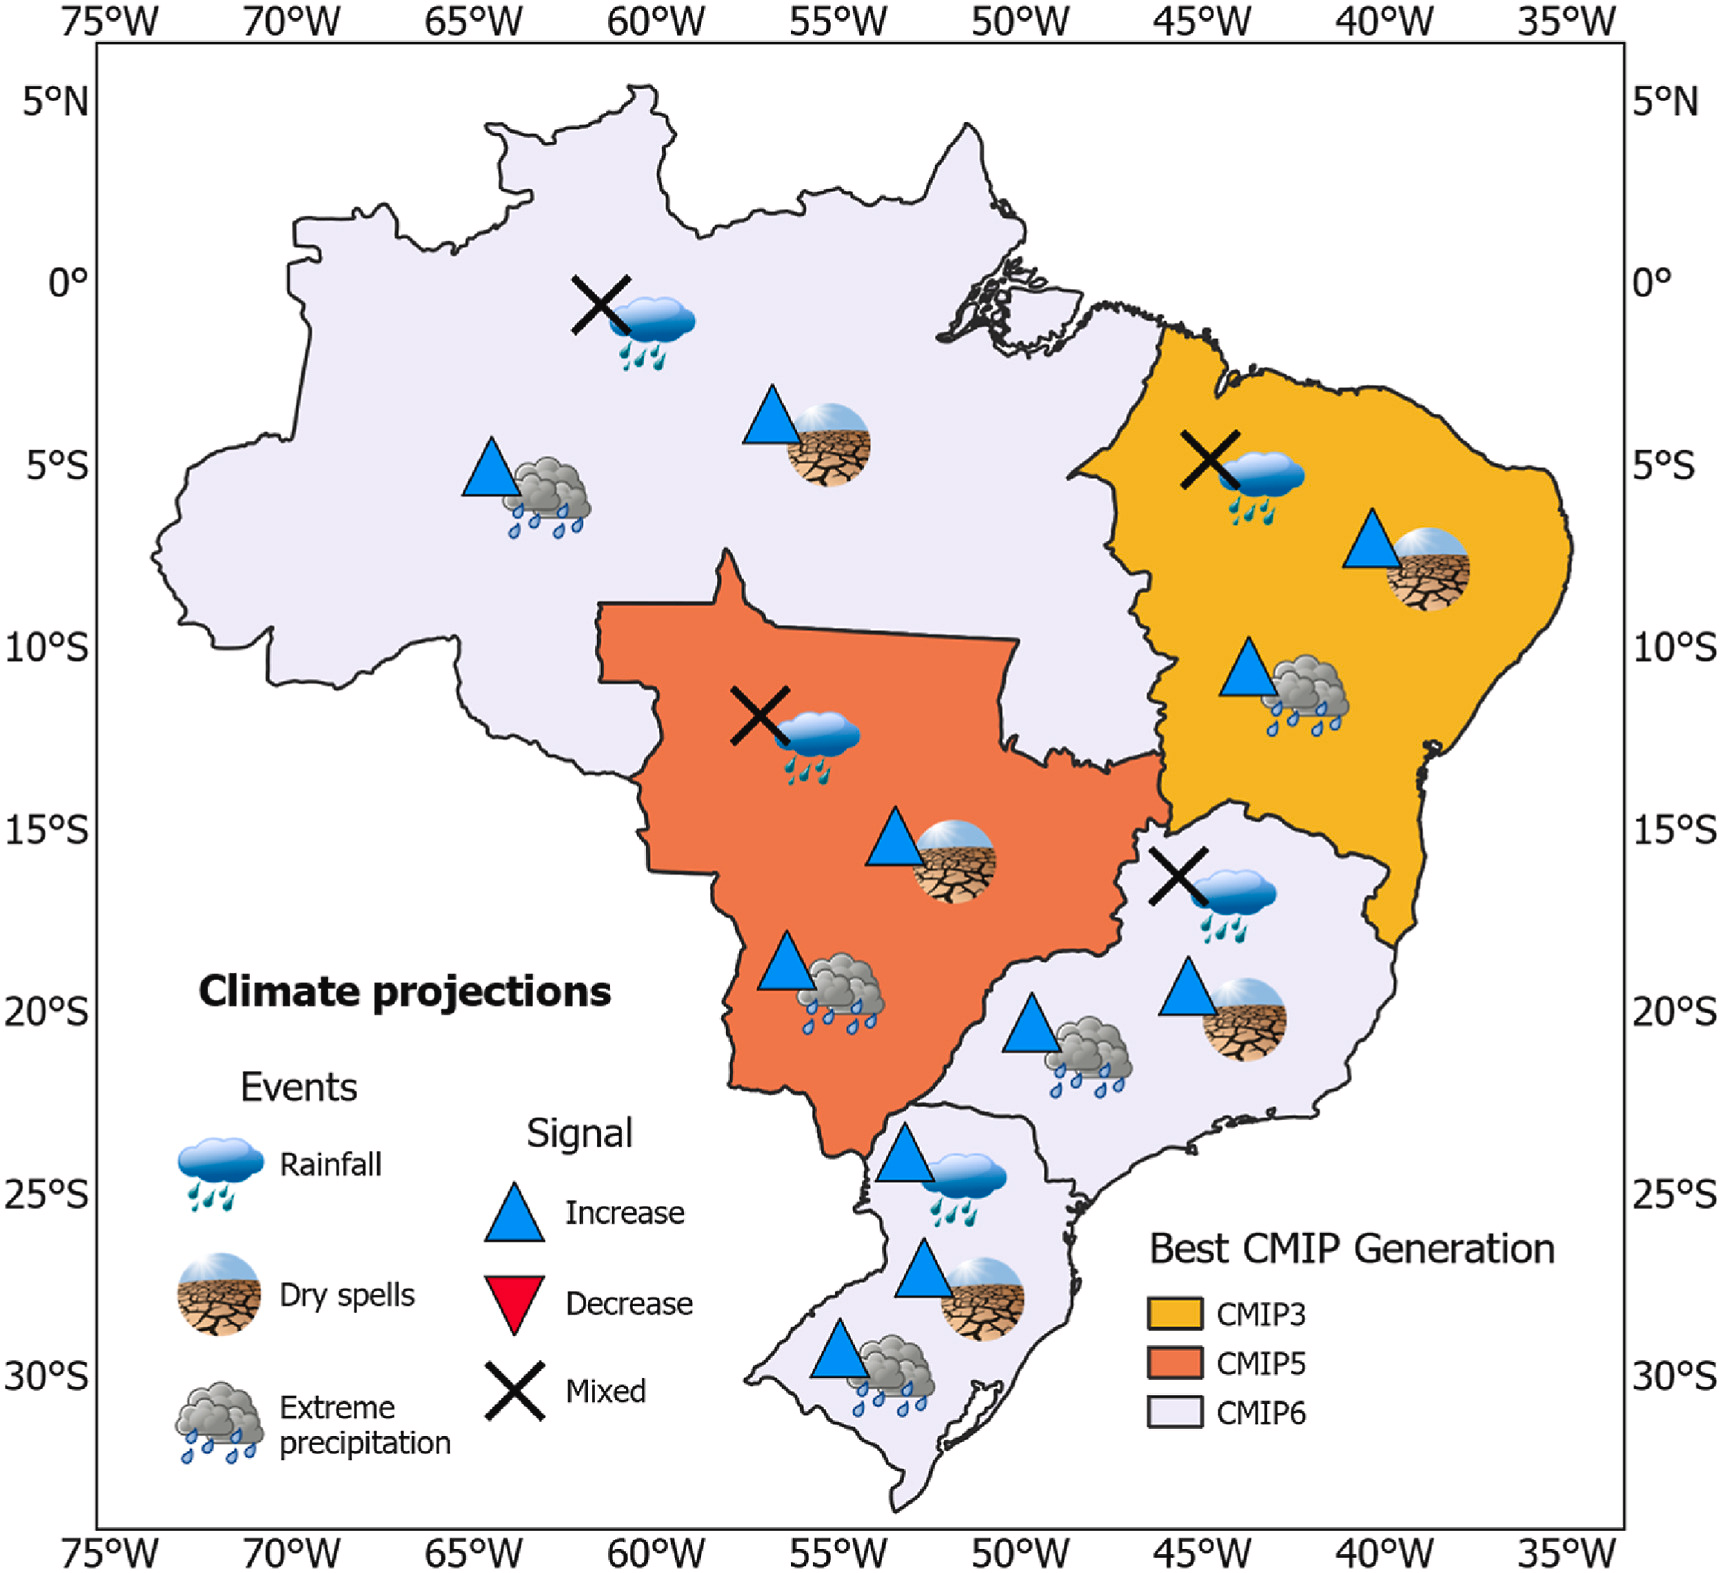
\includegraphics[width=\linewidth,height=0.78\textheight,keepaspectratio]{figuras/8e8716f29a7cc4852853ab4b941f6cec2bce73fa.png}
\caption{Resumo esquemático das principais mudanças projetadas nos extremos climáticos de precipitação nas regiões brasileiras. Extraído de (Medeiros; Oliveira; Avila-Diaz, 2022).}
\label{fig:figura-02}
\end{figure}

Nesse contexto de aumento de eventos extremos de precipitação na região Sul do Brasil, o estado do Rio Grande do Sul já vem, durante repetidos anos (2020, 2023, 2024), sofrendo com eventos de excesso de chuvas, desencadeando elevados prejuízos econômicos e sociais. (Porfírio da Rocha, Simões Reboita, Machado Crespo, 2024; Mantovani et al., 2024)

\section{Evento extremo de abril-maio de 2024 no Rio Grande do Sul}

Entre 26 de abril e 5 de maio de 2024, o estado do Rio Grande do Sul enfrentou um desastre hidrológico sem precedentes, desencadeado por eventos de precipitação extrema que superaram todos os registros históricos previamente observados. Todas as regiões hidrográficas do estado apresentaram elevados acumulados de chuva ao longo do período, no entretanto, a região hidrográfica do Guaíba concentrou os maiores volumes precipitados. Esse fato, associado à elevada densidade populacional da região (aproximadamente 6,8 milhões de habitantes, em contraste com cerca de 1,8 milhão na região hidrográfica do Uruguai e 1,1 milhão na região Litorânea) contribuiu para a intensificação dos impactos sobre a infraestrutura urbana e a população residente (MARENGO et al., 2024).

A extensão dos impactos refletiu-se diretamente no número e na distribuição das declarações oficiais de anormalidade dos municípios do estado. Até 30 de maio de 2024, 95 municípios decretaram estado de calamidade pública e 323 municípios declararam situação de emergência no estado (RIO GRANDE DO SUL, 2024).

Como pode ser observado na \textcolor{red}{Figura X,} a maior parte dos municípios que decretaram estado de calamidade pública estão localizados na região hidrográfica do Guaíba, corroborando a concentração espacial dos danos associados ao evento.

\begin{figure}[H]
\centering
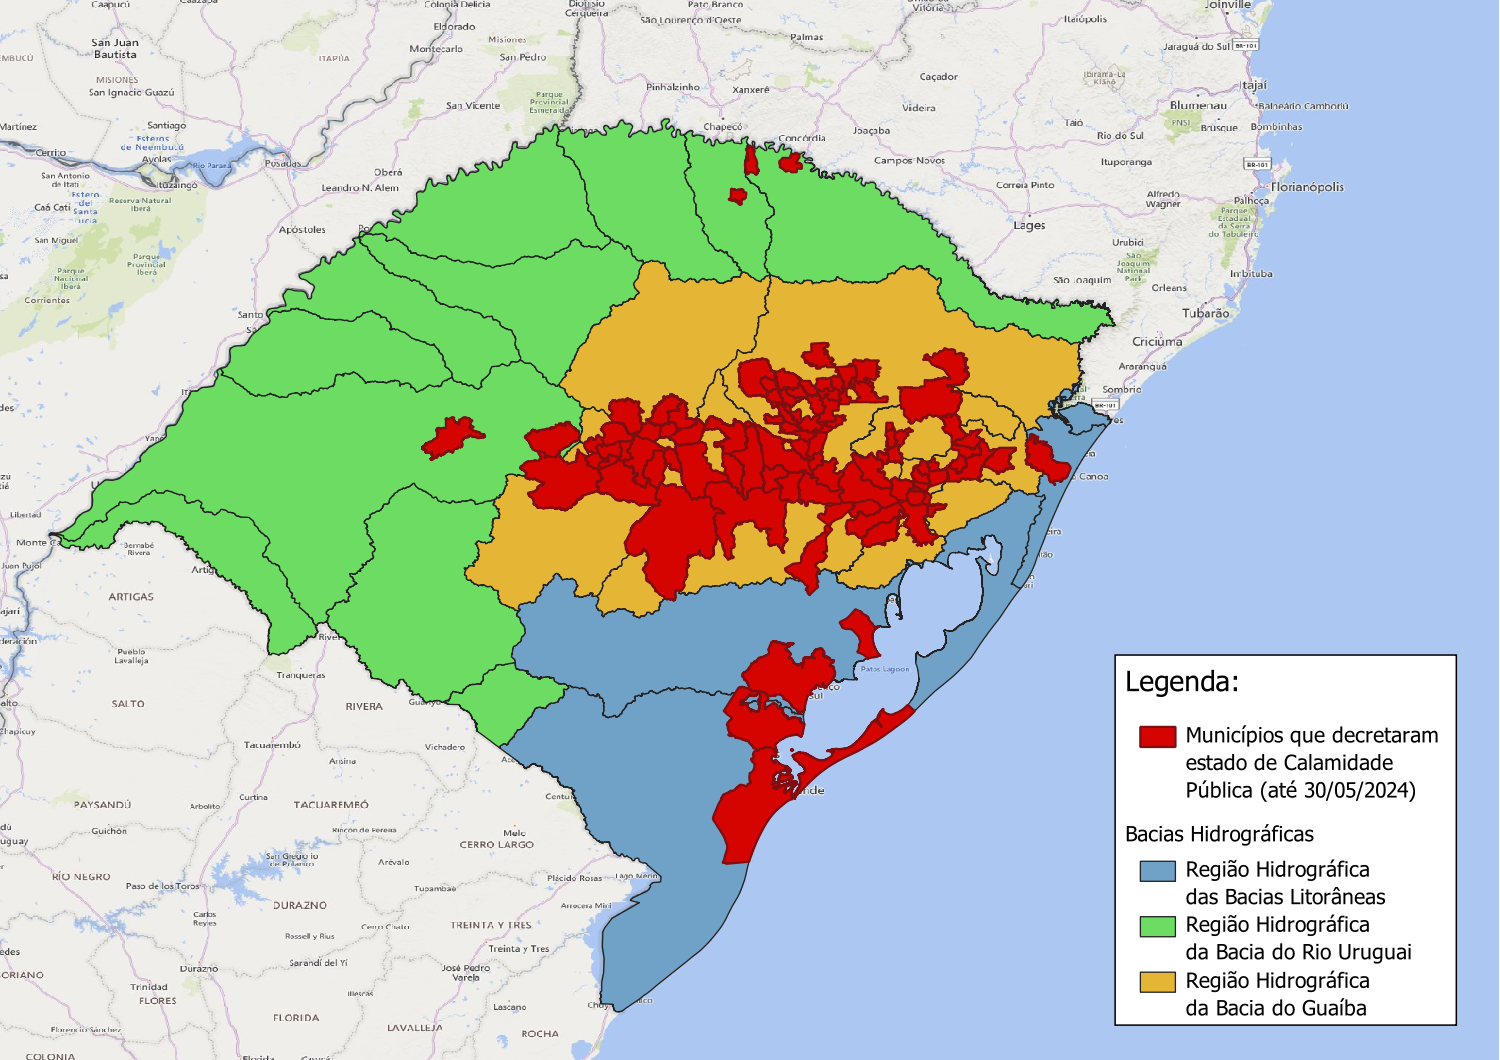
\includegraphics[width=\linewidth,height=0.78\textheight,keepaspectratio]{figuras/f9d087db07362eea968d6954aa342574b24ff6c2.png}
\caption{\textcolor{red}{Inserir legenda da figura.}}
\label{fig:figura-03}
\end{figure}

No município de Segredo, por exemplo, acumulados chegaram a 812,6 mm em 10 dias, enquanto Fontoura Xavier registrou 778 mm, volumes equivalentes a 280\% acima da média histórica para os meses de abril e maio. Essas precipitações elevaram o nível do Rio Guaíba a 5,35 metros em Porto Alegre \textcolor{red}{(figura 3)}, superando o recorde de 1941 (4,76 m) e alagando áreas urbanas de cidades como São Lourenço, Pelotas e Rio Grande, localizadas a mais de 400 km do epicentro das chuvas, além de diversas áreas rurais espalhadas por todo o estado (PORFÍRIO DA ROCHA; SIMÕES REBOITA; MACHADO CRESPO, 2024; FONSECA et al., 2024).

\begin{figure}[H]
\centering
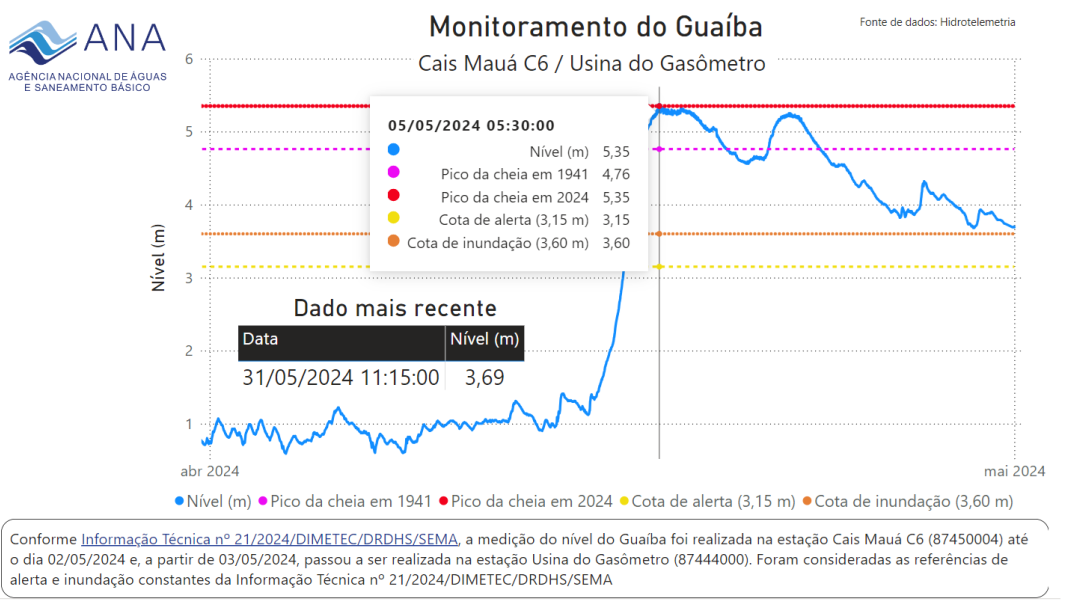
\includegraphics[width=\linewidth,height=0.78\textheight,keepaspectratio]{figuras/a6da75c003b48b87fafd0cd603fbb5e1fe94724e.png}
\caption{\textcolor{red}{Inserir legenda da figura.}}
\label{fig:figura-04}
\end{figure}

\subsection{Descrição dos mecanismos do evento}

Em níveis atmosféricos elevados (200 hPa), um anticiclone anômalo sobre o centro-sudeste do Brasil intensificou o jato subtropical \textcolor{red}{(figura 4)}, criando divergência de ar que favoreceu a formação de sistemas convectivos, pois a divergência de ar em altos níveis, ao retirar ar da coluna atmosférica, acaba contribuindo para a redução da pressão na superfície, o que, no caso desse evento, ocasionou o levantamento de ar quente e úmido, favorecendo assim a formação de nuvens (ROCHA; REBOITA; CRESPO, 2024).

\begin{figure}[H]
\centering
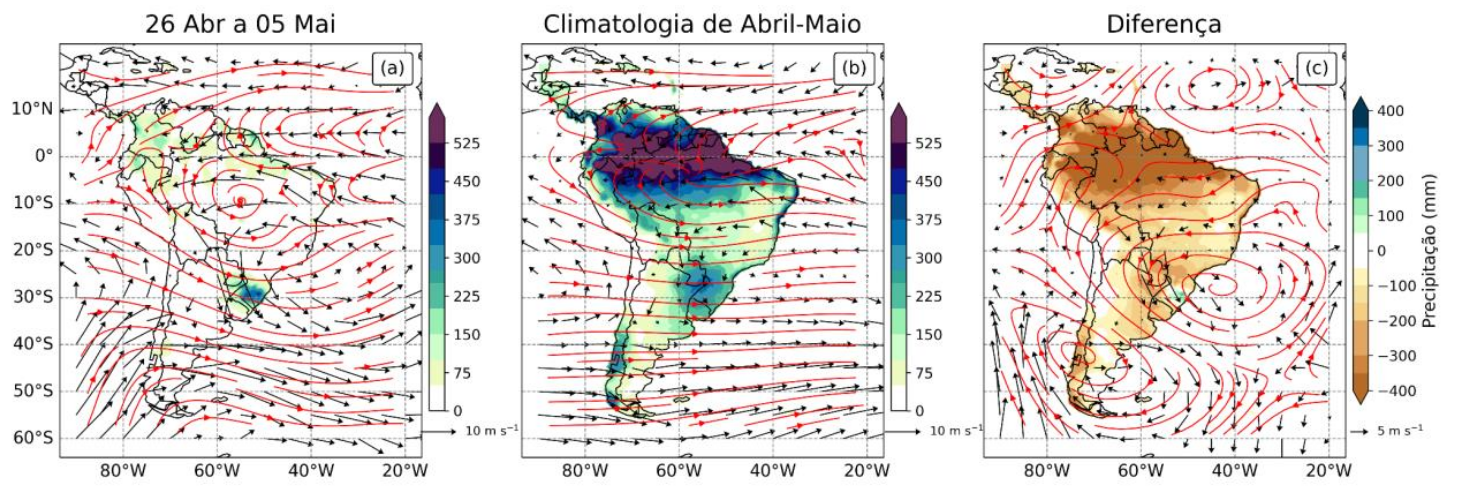
\includegraphics[width=\linewidth,height=0.78\textheight,keepaspectratio]{figuras/9215930ac95cb6eb7be04003f9474dbac6e5963f.png}
\caption{\textcolor{red}{Inserir legenda da figura.}}
\label{fig:figura-05}
\end{figure}

Simultaneamente, em baixos níveis (850 hPa), os ventos de norte/noroeste, fortalecidos pelo acoplamento da alta pressão anômala ao Anticiclone Subtropical do Atlântico Sul (\textcolor{red}{figura 4a, setas vermelhas}), transportaram umidade da Amazônia para o Rio Grande do Sul, alimentando de calor e umidade os baixos níveis atmosféricos sobre o Rio Grande do Sul (\textcolor{red}{figura, 4c, setas pretas}).

Além desses padrões anômalos sobre o continente, duas frentes frias (27-28 de abril e 1\textordmasculine{} de maio) influenciaram o direcionamento do jato de baixos níveis, transportando ar quente e úmido para a região Sul do Brasil. Esse processo contribuiu para a organização das chuvas e atuou como gatilho para o início das precipitações intensas do evento.

A persistência do padrão atmosférico por semanas foi reforçada por uma teleconexão com o oceano Índico, onde águas anormalmente quentes geraram ondas atmosféricas que ajudaram a manter o anticiclone sobre o Brasil central. A interação entre esses sistemas locais e globais resultou em chuvas contínuas e acumulados extremos (ROCHA; REBOITA; CRESPO, 2024).

\subsection{Abrangência e impactos socioeconômicos}

Esse evento afetou cerca de 5,6\% do território gaúcho, com danos significativos em 298 municípios, dos quais 34 tiveram mais de 20\% de suas áreas comprometidas por deslizamentos de terra, enxurradas, inundações e alagamentos. Nas zonas urbanas, 5\% da infraestrutura total foi impactada, com seis municípios registrando mais de 20\% de suas áreas urbanizadas afetadas (figura 5) (MAPBIOMAS, 2024).

A análises por imagens de satélite revelaram que 64,2\% das áreas atingidas eram terrenos agropecuários, como lavouras (39,1\%) e zonas de uso misto (24,2\%), seguidos por formações naturais não florestais, como campos e áreas pantanosas (25,4\%). Florestas e áreas não vegetadas representaram, respectivamente, 8\% e 2,4\% dos impactos (\textcolor{red}{tabela da figura 5}) (MAPBIOMAS, 2024 e DEFESA CIVIL DO RIO GRANDE DO SUL, 2024).

\begin{figure}[H]
\centering
\begin{minipage}{0.48\linewidth}\centering
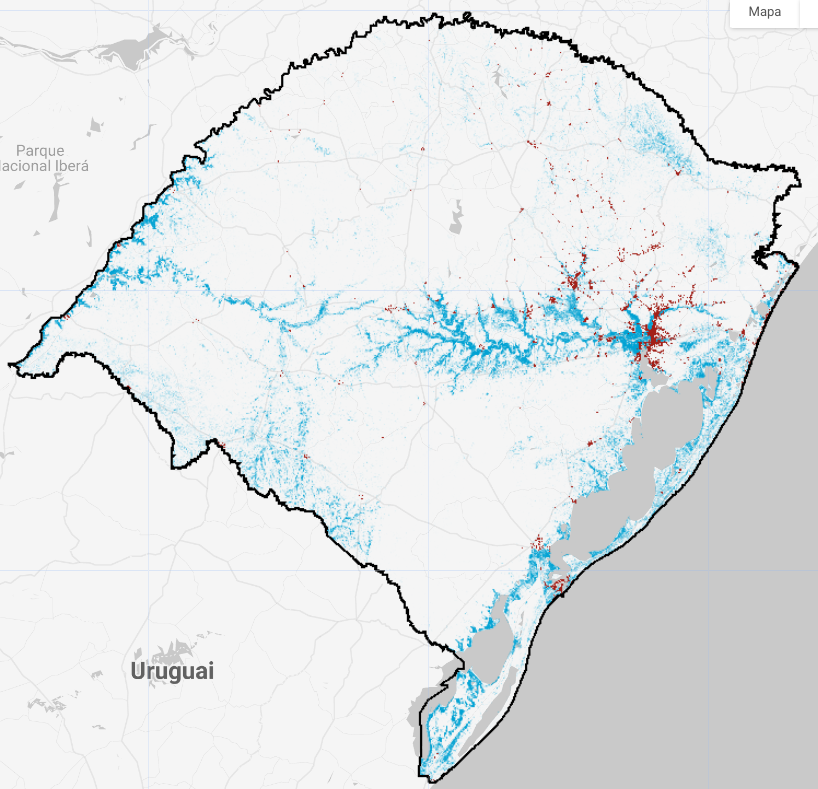
\includegraphics[width=\linewidth,height=0.40\textheight,keepaspectratio]{figuras/95e352d3eacc6cd736c96e360e1aa7c75f2687ce.png}
\end{minipage}\hfill
\begin{minipage}{0.48\linewidth}\centering
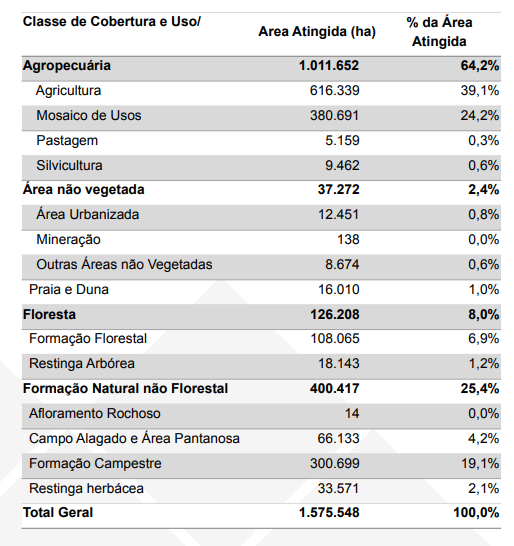
\includegraphics[width=\linewidth,height=0.40\textheight,keepaspectratio]{figuras/0c5e7a5a3517e4f990d1adf62c473805078809db.png}
\end{minipage}
\caption{\textcolor{red}{Inserir legenda da figura.}}
\label{fig:figura-06}
\end{figure}

Tamanha extensão de área afetada, combinada com a gravidade dos impactos em algumas regiões, resultaram em significativas perdas sociais, com a defesa civil estimando 2,4 milhões de afetados, 572 mil desalojados, 30 mil em abrigos, 31 desaparecidos e 182 mortes confirmadas (DEFESA CIVIL DO RIO GRANDE DO SUL, 2024).

A tragédia no Rio Grande do Sul também causou impactos econômicos significativos em diversos setores estaduais e nacionais. A Confederação Nacional do Comércio de Bens, Serviços e Turismo (2024) estimou que a perda no PIB do estado pode chegar a 9,08\% (R\$ 58,1 bilhões), com efeitos no PIB nacional de -1\% (R\$ 97 bilhões).

O mesmo relatório estimou também a perda de 305 mil empregos no total (195 mil no próprio estado e 110 mil no resto do Brasil). Os impactos discretizados por setor podem ser consultados na tabela 1.

\begin{figure}[H]
\centering
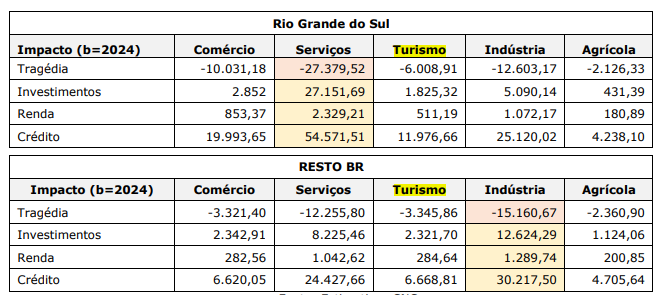
\includegraphics[width=\linewidth,height=0.78\textheight,keepaspectratio]{figuras/69f10093c8a36f93a213eef8761133852e758221.png}
\caption{\textcolor{red}{Inserir legenda da figura.}}
\label{fig:figura-07}
\end{figure}

\chapter{Justificativa}

Dado o histórico recente de eventos extremos de precipitação e a expectativa de aumento na frequência e intensidade dessas ocorrências no futuro (MARENGO et al., 2021), torna-se imprescindível dispor de previsões de curto prazo que sejam capazes de representar com precisão a distribuição espacial, a intensidade e a evolução temporal desses fenômenos.

Em regiões como o Rio Grande do Sul, onde já existe ocupação consolidada em áreas suscetíveis a inundações e onde projeções climáticas indicam que as cheias podem tornar-se até cinco vezes mais frequentes ao longo do século (PETRY et al., 2025), a capacidade de antecipar eventos de chuvas intensas é elemento fundamental para ações efetivas de mitigação, incluindo alertas antecipados, mobilização de defesa civil, evacuações preventivas e intervenções emergenciais em drenagem urbana (MARENGO et al., 2025; BUSKER et al., 2025; MARENGO et al., 2024).

Embora o foco deste trabalho seja a avaliação da capacidade preditiva de curto prazo, é importante destacar que o modelo abordado neste trabalho é um modelo atmosférico global, concebido para operar em múltiplos horizontes de previsão e, além de sua aplicação em previsões de tempo de alta resolução e curto prazo, ele pode também ser empregado em simulações sazonais, aproveitando sua capacidade de representar a circulação atmosférica em escala global com refinamento da grade para áreas de interesse.

No entanto, para que o modelo seja empregado com maior segurança em aplicações de médio e longo prazo, é importante avaliar, em primeiro lugar, sua capacidade de reproduzir adequadamente eventos extremos em horizontes temporais reduzidos, como os analisados neste estudo. Embora essa avaliação não seja suficiente para assegurar seu desempenho em escalas temporais mais longas, ela fornece uma evidência inicial sobre a representação dos processos físicos associados a eventos intensos, que também influenciam a habilidade do modelo em outros horizontes de previsão. De maneira complementar, Bauer, Thorpe e Brunet (2015) destacam que a habilidade em previsões de tempo e em previsões climáticas está relacionada à capacidade dos modelos de representar adequadamente os fenômenos meteorológicos e suas estatísticas, ainda que a previsibilidade e as métricas de avaliação variem conforme a escala temporal considerada.

Nesse sentido, trabalhos como este contribuem para a compreensão das potencialidades e limitações do modelo, servindo como base para investigações futuras voltadas à sua aplicação tanto em estudos de eventos de curto prazo quanto em análises de caráter de planejamento (SILVA et al., 2024).

\chapter{Fundamentação teórica e revisão bibliográfica}

\section{Previsão de tempo}

A previsão numérica de tempo baseia-se em modelos atmosféricos que representam, de forma discretizada, a evolução do estado da atmosfera a partir de condições iniciais e de contorno. Em sistemas modernos de previsão numérica, como esquematizado na figura X, o núcleo dinâmico calcula a evolução dos movimentos e processos resolvidos na escala da grade, enquanto parametrizações físicas representam processos sub-grade não resolvidos pela malha, como radiação, convecção e trocas turbulentas (Pu \& Kalnay, 2018).

Desta forma, a qualidade da previsão depende tanto da correta assimilação de dados de satélites, estações meteorológicas, aviões, etc, nas condições iniciais e de contorno do modelo, quanto da formulação física (diretamente resolvida ou parametrizada) e computacional do modelo (\href{https://www.ecmwf.int/sites/default/files/elibrary/2015/15259-modelling-infrastructure-integrated-forecasting-system-recent-advances-and-future-challenges.pdf}{Wedi et al., 2015;} Pu \& Kalnay, 2018).

\begin{figure}[H]
\centering
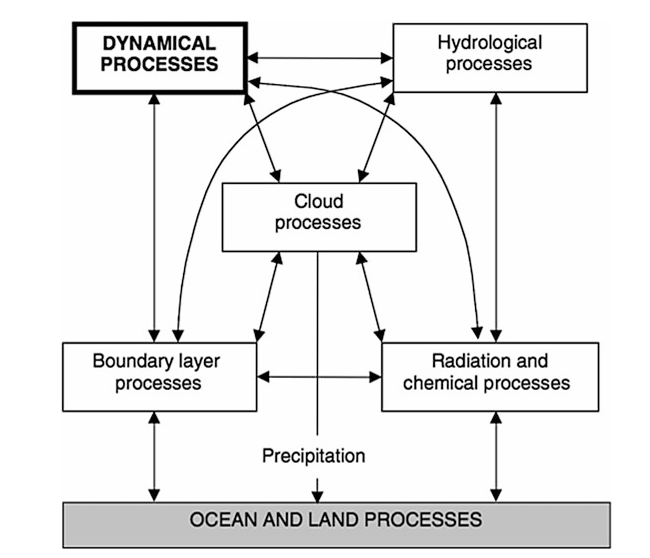
\includegraphics[width=\linewidth,height=0.78\textheight,keepaspectratio]{figuras/f7093e3c6eafe18ded70062fcb4462a71901142a.png}
\caption{Esquema dos processos físicos na atmosfera e suas interações. Os processos dinâmicos em escalas resolvíveis, destacados em negrito, são calculados diretamente pela dinâmica do modelo, enquanto os demais processos sub-grade são parametrizados com base nas variáveis da escala resolvida. Retirado de Pu \& Kalnay, 2018.}
\label{fig:figura-08}
\end{figure}

Esses modelos podem ser empregados em escalas globais ou regionais, conforme o domínio espacial, a resolução e o objetivo da aplicação. Modelos globais simulam a circulação atmosférica em todo o planeta em resoluções menores (devido ao custo computacional) e, por isso, são apropriados para representar fenômenos de grande escala e fornecer condições iniciais e de contorno para modelos regionais (ou seja, que não cobrem todo o globo).

O Integrated Forecasting System (IFS), do ECMWF, é apresentado como um sistema global de previsão numérica projetado para produzir previsões determinísticas e probabilísticas em horizontes que variam de vários dias até um ano. Ele consiste em um modelo de circulação geral atmosférica (o IFS-ST) acoplado a um sistema de assimilação de dados quadridimensional (4D-Var) para estabelecer o estado inicial do sistema terrestre (ROBERTS et al., 2018; KÜHNLEIN; SMOLARKIEWICZ, 2019). O Global Forecast System (GFS), do NCEP, é um sistema global de previsão numérica executado quatro vezes ao dia para gerar previsões de até 16 dias. O sistema utiliza o núcleo dinâmico Finite-Volume Cubed-Sphere (FV3), com resolução horizontal nominal de aproximadamente 13 km no componente atmosférico, e seus produtos são disponibilizados em diferentes grades, incluindo 0,25$^\circ$, 0,5$^\circ$ e 1,0$^\circ$. O GFS é inicializado pelo Global Data Assimilation System (GDAS), que fornece as condições iniciais da previsão (NCEP/EMC, 2026; NCEP/NCO, 2024).

Modelos regionais, por sua vez, são geralmente formulados como modelos de área limitada, aninhados sobre uma região de interesse. Por restringirem o domínio espacial de integração, podem ser executados em resoluções horizontais mais altas que modelos globais, sendo forçados por condições de contorno laterais provenientes desses modelos globais, análises ou reanálises atmosféricas (GIORGI; MEARNS, 1999; DAVIES, 2014).

Essa estratégia, de aninhamento e downscaling dinâmico, permite representar com maior detalhe efeitos de orografia, contraste terra-mar e processos atmosféricos de menor escala, conforme ilustrado esquematicamente na \textcolor{red}{Figura X}.

\begin{figure}[H]
\centering
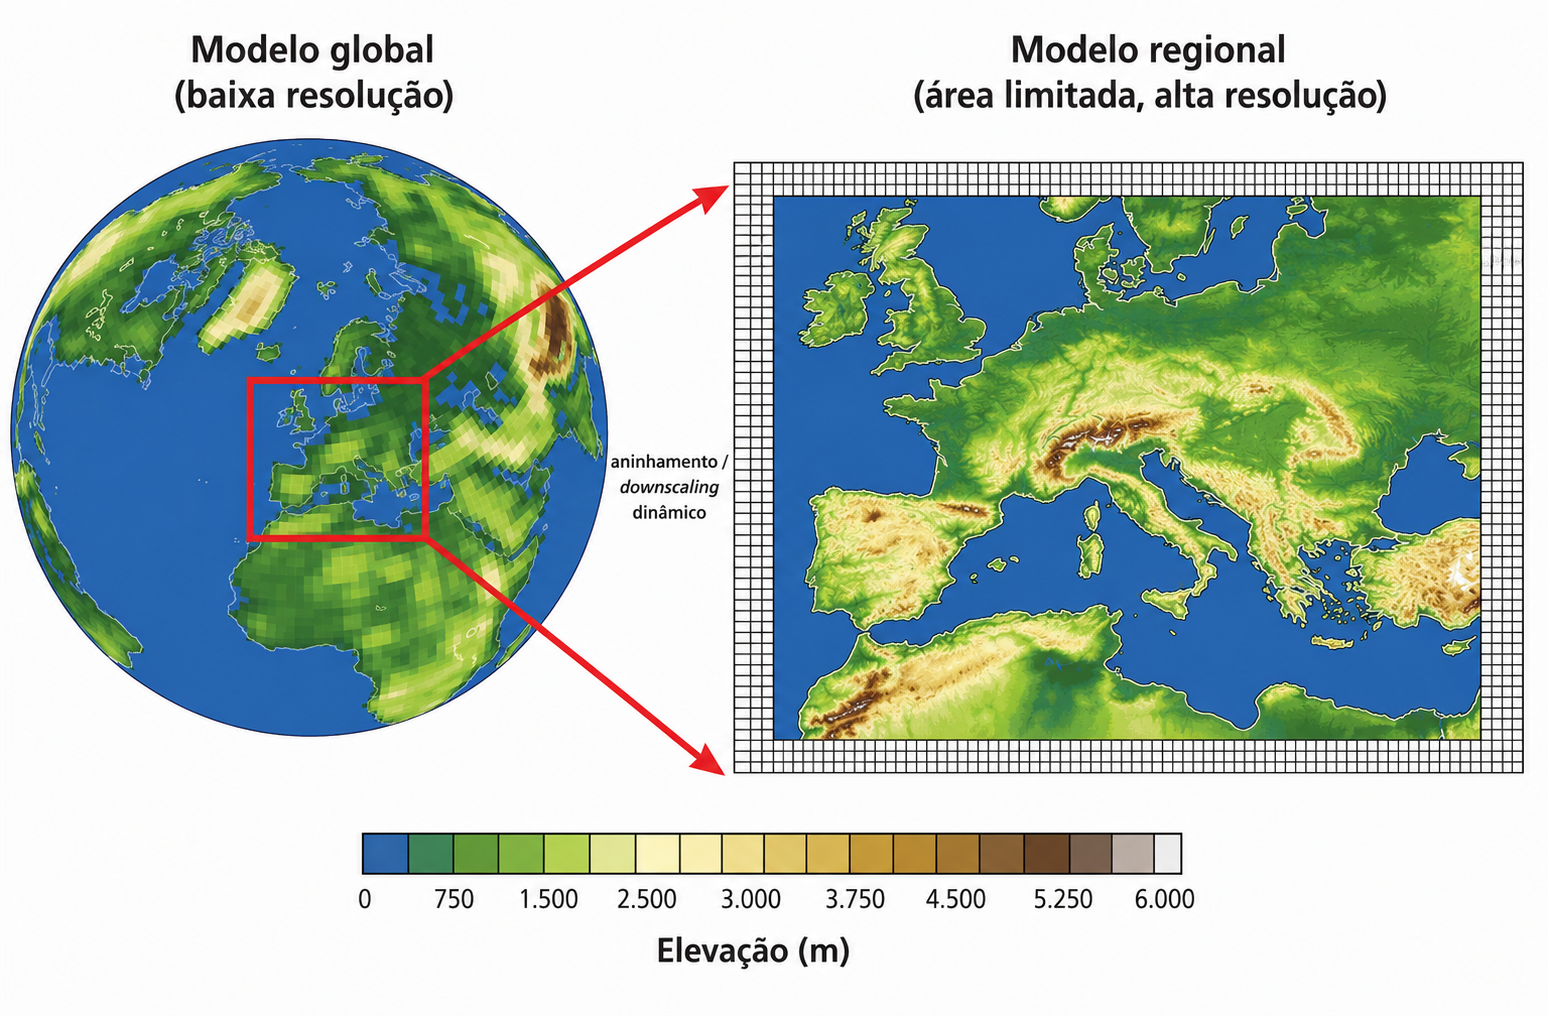
\includegraphics[width=\linewidth,height=0.78\textheight,keepaspectratio]{figuras/a2bd9fd4c7cdca5b79d47d1ff01a0186f41ee8a7.png}
\caption{Representação esquemática do aninhamento de um modelo regional em um modelo global, com aumento da resolução espacial sobre a região de interesse.}
\label{fig:figura-09}
\end{figure}
Fonte: adaptado de Giorgi e Gutowski Jr. (2015).

A utilidade dos modelos regionais decorre, portanto, da melhor representação de fenômenos meteorológicos com domínio em escalas espaciais menores, embora seu desempenho dependa da aplicação, da variável analisada, do domínio de integração e da qualidade das condições fornecidas pelo modelo de grande escala (FESER et al., 2011; TAPIADOR et al., 2020). Assim, enquanto modelos globais são fundamentais para representar a circulação de grande escala e fornecer condições aos modelos regionais, estes são empregados para detalhar processos atmosféricos em domínios espaciais mais restritos.

Entre os modelos regionais, o Eta é um exemplo de modelo aplicado à América do Sul em domínio regional que utiliza a coordenada vertical \emph{eta} ou \emph{step-mountain}, com topografia representada em degraus, recurso associado à redução de erros no cálculo de derivadas horizontais em terrenos inclinados (\href{http://climanalise.cptec.inpe.br/~rclimanl/revista/pdf/ETA_Chou.pdf}{Chou; Justi da Silva, 1999}). Já o BRAMS é derivado do RAMS (Regional Atmospheric Modeling System) e foi desenvolvido no Brasil como um sistema regional integrado para tempo, química atmosférica e ciclo do carbono, com aplicações operacionais e de pesquisa principalmente na América do Sul (\href{https://gmd.copernicus.org/articles/10/189/2017/}{Freitas et al., 2017}).

O MPAS, por sua vez, representa uma alternativa à separação clássica entre modelos globais e regionais, pois utiliza uma grade não estruturada de resolução variável. Com isso, permite manter um domínio global e concentrar maior resolução sobre regiões específicas, reduzindo problemas relacionados às conexões entre grades de diferentes resoluções, comuns em modelos regionais aninhados (SKAMAROCK et al., 2012; PARK et al., 2014).

Assim, a previsão de tempo operacional e científica combina modelos globais, que capturam a evolução da circulação atmosférica de grande escala e fornecem orientação de médio prazo, com modelos regionais, que refinam a informação em domínios específicos e buscam representar processos locais com maior detalhe. A escolha entre GFS, ECMWF/IFS, MPAS, Eta, BRAMS ou outro sistema depende então do objetivo da previsão, do domínio espacial, da resolução necessária e da disponibilidade computacional (\href{https://www.ecmwf.int/sites/default/files/elibrary/2015/15259-modelling-infrastructure-integrated-forecasting-system-recent-advances-and-future-challenges.pdf}{Wedi et al., 2015}; \href{https://www.hereon.de/imperia/md/content/gkss/zentrale_einrichtungen/bibliothek/journals/2011/feser_29114.pdf}{Feser et al., 2011}).

\section{ETA}

O Eta é um modelo atmosférico regional de malha horizontalmente regular, desenvolvido originalmente na Universidade de Belgrado em conjunto com o Instituto de Hidrometeorologia da antiga Iugoslávia e posteriormente operacionalizado no National Centers for Environmental Prediction (NCEP). Sua formulação inicial está associada à coordenada vertical eta e à representação da topografia em degraus, descritas nos trabalhos de Mesinger (1984) e Mesinger et al. (1988) e posteriormente incorporadas à versão operacional do NMC/NCEP apresentada por Black (1994).

No Brasil, o modelo foi instalado no Centro de Previsão de Tempo e Estudos Climáticos do Instituto Nacional de Pesquisas Espaciais (CPTEC/INPE) em 1996, com o objetivo de complementar as previsões do modelo global e fornecer maior detalhamento espacial sobre a América do Sul (Lyra et al., 2022).

Por ser um modelo regional, o Eta não substitui o modelo global, mas atua como um refinamento regional das condições atmosféricas fornecidas. Essa característica permite representar com maior detalhe processos de mesoescala e efeitos regionais associados à orografia, frentes, brisas marítimas, sistemas convectivos e tempestades severas. Segundo o manual do Modelo Eta, o sistema é utilizado no INPE em diferentes escalas temporais, incluindo previsão de tempo, previsão sazonal e simulações climáticas de longo prazo, além de aplicações em setores como agricultura, energia hidrelétrica, energia eólica, eventos extremos e estudos ambientais (Lyra et al., 2022).

A principal característica do Eta é o uso da coordenada vertical \ensuremath{\eta}, que dá nome ao modelo. Diferentemente de coordenadas que acompanham diretamente a superfície do terreno, a coordenada eta reduz a inclinação das superfícies coordenadas em áreas de relevo acentuado. Essa formulação foi proposta para reduzir erros numéricos no cálculo da força do gradiente horizontal de pressão em regiões montanhosas, problema particularmente relevante em domínios com topografia complexa, como a Cordilheira dos Andes (Mesinger, 1984; Mesinger et al., 1988; Mesinger et al., 2012; Lyra et al., 2022). Essa propriedade explica parte da adequação do Eta para aplicações sobre a América do Sul, onde o contraste entre a Cordilheira dos Andes, as terras baixas amazônicas e os planaltos brasileiros impõe forte heterogeneidade ao escoamento atmosférico.

\begin{figure}[H]
\centering
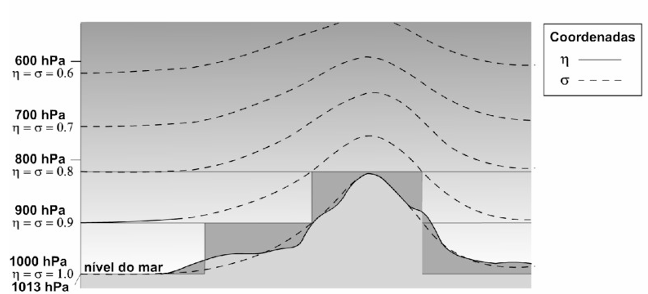
\includegraphics[width=\linewidth,height=0.78\textheight,keepaspectratio]{figuras/2d11499d71fc765d49c7143b4b6c54e6bc8a17f3.png}
\caption{Representação esquemática das coordenadas verticais eta (\ensuremath{\eta}) e sigma (\ensuremath{\sigma}) em região de topografia acentuada. Fonte: Lyra et al. (2022).}
\label{fig:figura-10}
\end{figure}

Do ponto de vista da discretização horizontal, o modelo utiliza a grade E de Arakawa, na qual pontos de massa e de vento são dispostos de forma alternada, já a dinâmica do Eta, combina a coordenada vertical eta com uma formulação numérica conservativa, associada aos esquemas de diferenças de Arakawa e à conservação de propriedades dinâmicas relevantes, como energia e enstrofia, conforme descrito por Mesinger et al. (2012).

A integração temporal do Eta utiliza uma formulação do tipo \emph{split-explicit}, na qual os processos atmosféricos mais rápidos, associados ao ajuste por ondas de gravidade, são tratados separadamente dos processos de transporte advectivo, que evoluem em escalas de tempo relativamente mais lentas. Essa estratégia permite manter a estabilidade numérica do modelo sem impor o mesmo passo de tempo restritivo a todos os termos das equações, enquanto as condições de contorno são prescritas nas bordas do domínio e atualizadas a partir do modelo forçante (Mesinger et al., 2012; Lyra et al., 2022).

\begin{figure}[H]
\centering
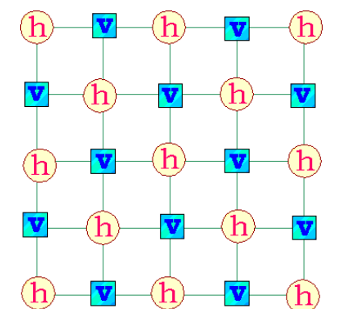
\includegraphics[width=\linewidth,height=0.78\textheight,keepaspectratio]{figuras/fdc85933e293525e3221953d6e5282389620562d.png}
\caption{Distribuição horizontal das variáveis na grade E de Arakawa utilizada no Modelo Eta, onde `h' representa a variável de massa e `v' representa as componentes horizontais do vento. Fonte: Lyra et al. (2022).}
\label{fig:figura-11}
\end{figure}

Ao longo do tempo, o código do Eta passou por atualizações importantes. Mesinger et al. (2012) sintetizam uma versão aprimorada do modelo, originada a partir do Workstation Eta do NCEP e disponibilizada pelo CPTEC. Entre os principais aprimoramentos estão a introdução dos chamados \emph{sloping steps que é} uma forma discretizada de topografia do tipo \emph{shaved cells,} a adoção de advecção vertical por volume finito para variáveis dinâmicas, a inclusão do carregamento de vapor e hidrometeoros na equação hidrostática, ajustes no cálculo dos coeficientes de troca, melhorias na conservação da difusão vertical, modificações no diagnóstico de ventos a 10 m, e refinamentos nos esquemas de convecção (Mesinger et al., 2012). Esses avanços foram motivados tanto por limitações identificadas em simulações anteriores quanto pela incorporação de processos fisicamente justificáveis que ainda não estavam presentes no código.

A física do Eta reúne parametrizações para processos subgrade de convecção, microfísica, radiação, superfície e turbulência. Na versão descrita por Mesinger et al. (2012), o pacote físico inclui opções de convecção Betts-Miller-Janjic e Kain-Fritsch, microfísica de Ferrier, esquemas de radiação do GFDL, modelo de superfície Noah, similaridade de Monin-Obukhov na camada superficial, arrasto orográfico dependente da direção do vento e fechamento de turbulência Mellor-Yamada 2.5. Esses componentes são relevantes porque a habilidade do modelo não depende apenas do núcleo dinâmico, mas também da forma como processos convectivos, trocas superfície-atmosfera, camada limite e outros processos não resolvidos diretamente pelas equações na escala da grade são parametrizados.

As condições iniciais e de contorno constituem outro ponto central para a interpretação do desempenho do Eta. O manual do modelo descreve que, na configuração recente do INPE, a condição inicial é obtida a partir da análise do GFS, interpolada para a grade do Eta. A temperatura da superfície do mar é mantida constante em integrações de curto prazo e atualizada em integrações climáticas, enquanto as condições de contorno laterais são atualizadas a cada seis horas com previsões do modelo global. Além disso, o aninhamento é do tipo \emph{one-way}, ou seja, o modelo regional recebe informação do modelo forçante, mas não retroalimenta o modelo global (Lyra et al., 2022). Portanto, a previsão regional pode refinar padrões espaciais e processos de mesoescala, mas permanece limitada pela qualidade da circulação de grande escala imposta pelas condições iniciais e de contorno.

Em uma avaliação voltada a chuvas intensas, Vieira et al. (2015) analisaram previsões do Eta-8 km e Eta-40 km para 25 eventos na bacia do Rio São Francisco, a montante da UHE Três Marias, com antecedência de 72 horas. A avaliação combinou métricas objetivas, como BIAS e ETS, com análise subjetiva de campos sinóticos. Os autores observaram que o Eta-8 km apresentou melhor desempenho que o Eta-40 km para previsão de chuva diária moderada a forte, embora tenha pior desempenho para chuva fraca. No entanto, em alguns casos, os máximos observados de precipitação não foram plenamente reproduzidos, indicando que o aumento de resolução não elimina limitações na representação da intensidade dos eventos. Além disso, quando o modelo global do CPTEC/INPE errou o posicionamento do sistema meteorológico atuante, as previsões do Eta também foram afetadas (Vieira et al., 2015). Assim, o aumento de resolução melhora alguns aspectos da previsão, mas não elimina erros herdados da condição de contorno nem garante a correta intensidade dos extremos.

Além da previsão de tempo, o Eta tem sido amplamente empregado como modelo regional climático para a América do Sul. Chou et al. (2005) avaliaram previsões sazonais de precipitação do Eta sobre a América do Sul e mostraram que a habilidade do sistema varia conforme a região, estação e escala temporal avaliada. Pesquero et al. (2010) e Chou et al. (2012) utilizaram o Eta para downscaling climático do clima presente sobre a América do Sul, enquanto Marengo et al. (2012) aplicaram o sistema Eta-CPTEC/HadCM3 para a construção de cenários regionais futuros, com análises para as bacias Amazônica, São Francisco e Paraná. Em conjunto, esses estudos indicam que o Eta é capaz de agregar detalhamento regional às simulações globais, embora ainda apresente vieses regionais de precipitação e temperatura, especialmente em áreas onde a convecção, a topografia e a circulação de grande escala interagem de forma complexa.

A revisão indica que, no geral, o Modelo Eta imlementado no CPTEC apresenta uma formulação adequada à modelagem regional na América do Sul, principalmente pela combinação entre a coordenada eta, representação da topografia e sua aplicação em diferentes escalas temporais. No entanto, os estudos avaliados mostram que esse detalhamento regional não elimina limitações associadas à qualidade das condições iniciais e de contorno, às parametrizações físicas e à resolução espacial adotada. Dessa forma, sua utilização deve ser acompanhada por avaliações específicas para cada região, período e tipo de evento, especialmente em aplicações voltadas à precipitação intensa, nas quais erros de posicionamento, suavização dos máximos e vieses sistemáticos podem afetar a qualidade da previsão.

\section{BRAMS}

O BRAMS (\emph{Brazilian developments on the Regional Atmospheric Modeling System}) é um modelo atmosférico regional de malha horizontalmente regular, derivado do RAMS (\emph{Regional Atmospheric Modeling System}), desenvolvido originalmente na Colorado State University para simular circulações atmosféricas em múltiplas escalas (Pielke et al., 1992; Cotton et al., 2003). No Brasil, o desenvolvimento do BRAMS foi iniciado por um consórcio envolvendo a ATMET, o IME/USP, o IAG/USP e o CPTEC/INPE, com financiamento da FINEP, com o objetivo de adaptar o RAMS às necessidades de previsão e pesquisa em regiões tropicais e subtropicais (Freitas et al., 2017).

Ao longo de seu desenvolvimento, o BRAMS incorporou módulos voltados à química atmosférica, aerossóis, transporte de traçadores, emissões de queimadas, superfície continental e ciclo do carbono, deixando de atuar apenas como modelo meteorológico regional. O CATT-BRAMS permitiu representar transporte, dispersão, transformação química e remoção de gases e aerossóis de forma acoplada à meteorologia simulada (Freitas et al., 2009; Longo et al., 2010), enquanto o acoplamento com o JULES ampliou a representação de fluxos de água, energia e carbono sobre a América do Sul (Moreira et al., 2013) e, na versão 5.2, esses desenvolvimentos foram reunidos em um sistema integrado, com atualização de parametrizações físicas e melhorias computacionais (Freitas et al., 2017).

Do ponto de vista dinâmico, o BRAMS é um modelo regional não hidrostático e compressível, cuja formulação deriva das equações não hidrostáticas compressíveis descritas por Tripoli e Cotton (1982), conforme descrito em Freitas et al. (2017).

O modelo utiliza grade C de Arakawa na horizontal e grade de Lorenz na vertical, podendo empregar coordenada vertical cartesiana ou coordenadas que acompanham o terreno (\emph{terrain-following height}), além de coordenada horizontal cartesiana ou projeção polar estereográfica rotacionada. No BRAMS 5.2, também foi incorporada a opção de uma formulação conservativa em massa para a equação da função de Exner, em consonância com a discussão sobre conservação de massa em simulações regionais apresentada por Medvigy et al. (2005). Por ser um modelo regional, sua integração depende de condições iniciais e de contorno fornecidas por análises ou previsões de modelos de maior escala. Na configuração operacional do CPTEC/INPE, as previsões regionais de 5 km são inicializadas a partir do GFS/NCEP, com pré-processamento pelo RAMS-ISAN, cobrindo a América do Sul e oceanos adjacentes (Freitas et al., 2017).

\begin{figure}[H]
\centering
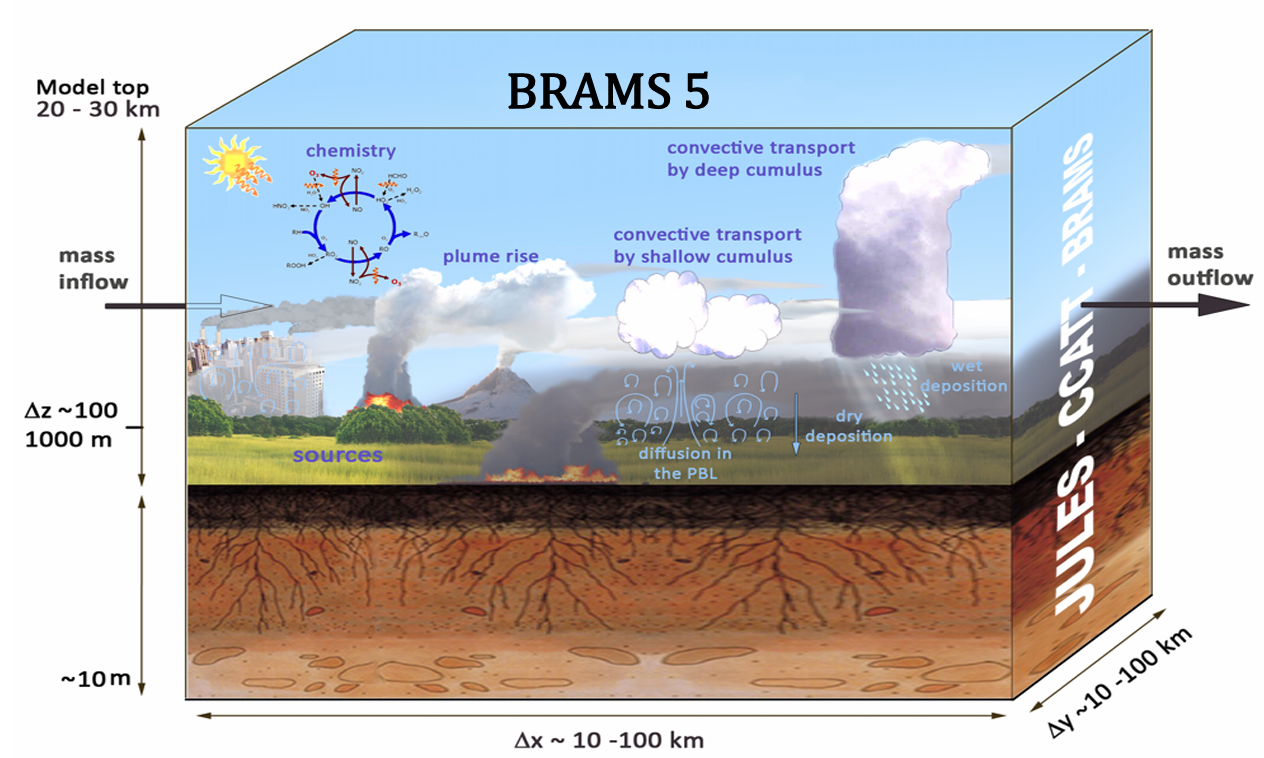
\includegraphics[width=\linewidth,height=0.78\textheight,keepaspectratio]{figuras/e2fd150cd1c5e96f066d877acb9e8fec103fa0e5.png}
\caption{Esquema conceitual dos processos físicos e químicos representados no BRAMS 5.2, incluindo transporte convectivo, química atmosférica, elevação de plumas, deposição seca e úmida e interação com a superfície. Fonte: Freitas et al. (2016), reproduzido.}
\label{fig:figura-12}
\end{figure}

A física do modelo reúne parametrizações de microfísica, radiação, turbulência, convecção, superfície e química atmosférica. No caso da convecção, componente particularmente sensível em regiões tropicais e também para esse estudo, o BRAMS incorporou a parametrização de Grell e Dévényi (2002), baseada em fluxo de massa e em múltiplos fechamentos convectivos. Essa estrutura permite gerar um ensemble físico dentro do próprio modelo. Posteriormente, Grell e Freitas (2014) propuseram uma parametrização convectiva estocástica, sensível à escala e a aerossóis, adequada a aplicações em previsão de tempo e qualidade do ar, especialmente em resoluções nas quais parte da convecção é resolvida explicitamente e parte ainda depende de parametrização.

De forma mais aderente ao escopo desse trabalho, o BRAMS tem sido utilizado em estudos de downscaling e eventos extremos onde, por exemplo, García Villanueva e Sutizal Sánchez (2017) aplicaram o BRAMS 4.2 ao evento de huaico de Chosica, em Lima, Peru, ocorrido em março de 2015, utilizando dados do modelo global do CPTEC como entrada para três domínios aninhados, com resoluções de 64 km, 16 km e 2 km. Os autores observaram que a precipitação prevista com cinco dias de antecedência apresentou aumento altitudinal até aproximadamente 1500 m e redução acima desse nível, padrão também identificado nos dados observados. O resultado foi associado à atuação de ventos provenientes do Pacífico, à topografia e à instabilidade potencial da atmosfera, mas deve ser interpretado como estudo de caso, e não como avaliação geral do modelo.

No quesito desempenho, diferentes avaliações indicam que a habilidade do BRAMS varia conforme variável, região, resolução e configuração física. Freitas et al. (2017) avaliaram previsões operacionais do BRAMS em grade de 5 km entre janeiro de 2013 e janeiro de 2015 e observaram desempenho satisfatório para regiões tropicais e subtropicais da América do Sul, embora com maiores erros em temperatura durante a estação seca e menor habilidade para limiares mais elevados de precipitação. Em avaliação na Amazônia oriental, Moraes et al. (2013) compararam BRAMS, Eta e GFS nos meses chuvosos de janeiro a abril de 2012 e observaram erros de superestimativa e subestimativa da chuva, sobretudo no centro-norte do Pará e no Amapá. Nesse caso específico, o GFS apresentou melhor desempenho geral, enquanto o BRAMS mostrou limitações na representação da precipitação em parte da região analisada.

Ao longo das últimas duas décadas, o BRAMS se consolidou como um sistema regional de previsão e pesquisa voltado a aplicações meteorológicas e ambientais, especialmente na América do Sul. Sua evolução a partir do RAMS permitiu incorporar processos relevantes para regiões tropicais e subtropicais, mas seu desempenho permanece condicionado à resolução, às condições iniciais e de contorno, às parametrizações físicas e à variável analisada. Por isso, embora seja um modelo operacional e amplamente aplicado, sua utilização em estudos de previsão ou avaliação de eventos extremos deve ser sempre acompanhada de validação específica para o domínio, período e fenômeno investigado.

\section{Modelo MPAS (Model Prediction Across Scales)}

O Model for Prediction Across Scales (MPAS), em seu componente atmosférico MPAS-A, é um modelo atmosférico global de resolução variável desenvolvido para representar processos atmosféricos em múltiplas escalas dentro de um mesmo domínio computacional. Diferentemente de modelos globais baseados em grades latitude-longitude regulares ou de modelos regionais aninhados em domínios espacialmente limitados, o MPAS utiliza uma malha global não estruturada, baseada em Tesselações Esféricas Centroidais de Voronoi (TECV, ou SCVT), que permite concentrar maior resolução espacial em regiões de interesse e manter resolução mais grosseira no restante do globo (Skamarock et al., 2012; Ringler et al., 2011; MPAS Development Team, 2026b).

O desenvolvimento do MPAS está associado à busca por alternativas aos principais limites da modelagem atmosférica global e regional. Em modelos globais de grade regular, o refinamento de uma área específica tende a exigir aumento de resolução em todo o planeta, elevando fortemente o custo computacional. Já em modelos regionais, o refinamento espacial depende de condições de contorno laterais provenientes de um modelo externo, o que pode introduzir inconsistências nas bordas do domínio e afetar a propagação de ondas e sistemas meteorológicos de grande escala. A proposta do MPAS é justamente combinar a consistência de um domínio global com a capacidade de refinamento regional contínuo, permitindo que a região refinada permaneça dinamicamente conectada à circulação planetária sem a necessidade de fronteiras laterais mais instáveis, como nos aninhamentos tradicionais (Skamarock et al., 2012; Hagos et al., 2013; Park et al., 2014).

A documentação oficial descreve o MPAS como um framework comum de modelagem de tempo e clima, de código aberto e núcleo atmosférico (MPAS-A) desenvolvido no âmbito do NCAR, além de outros componentes associados a outras instituições (MPAS Development Team, 2026a; MPAS Development Team, 2026b). Assim, embora o foco desta revisão seja o MPAS-A, o modelo deve ser entendido como parte de uma infraestrutura mais ampla de modelagem multiescala.

Essa condição é relevante no contexto brasileiro recente porque o MPAS-A passou a constituir a base do componente atmosférico do MONAN (Model for Ocean-laNd-Atmosphere predictioN), que é uma iniciativa comunitária liderada pelo INPE e pelo MCTI, voltada ao desenvolvimento de um sistema unificado de modelagem do Sistema Terrestre, capaz de produzir previsões e simulações em diferentes escalas temporais e espaciais, e que tem como seu foco a modelagem na América do Sul. A página oficial do projeto descreve o MONAN como um modelo comunitário que agrega instituições brasileiras e colaboradores externos, com estrutura inicial baseada no núcleo dinâmico do MPAS 8.0.1 e com parte da física derivada do próprio MPAS e parte incorporada ou desenvolvida pela comunidade (MONAN, 2026; Fusinato, 2025).

A escolha do MPAS como base do MONAN-ATM decorreu de uma avaliação de candidatos a núcleo dinâmico, que incluiu o GEF, FV3/SHiELD e o próprio MPAS. Os candidatos foram analisados tanto por critérios computacionais, como manutenibilidade, portabilidade, performance, escalabilidade e eficiência, quanto por critérios de funcionalidade e adequação meteorológica. A recomendação encaminhada ao Comitê Científico do MONAN propôs o MPAS como base do núcleo dinâmico e da estrutura de dados do componente atmosférico, mantendo inicialmente as parametrizações físicas e o modelo superfície-atmosfera embarcados no MPAS como ponto de partida para os desenvolvimentos posteriores da comunidade MONAN (Freitas, 2023; Rodrigues et al., 2023).

Dessa forma, o MONAN amplia a relevância do MPAS-A para o Brasil e, assim, o modelo deixa de ser apenas uma alternativa multiescala avaliada em estudos acadêmicos e passa a compor a base de uma infraestrutura nacional de previsão e pesquisa (Freitas, 2023).

Por ser um modelo global de resolução variável, o MPAS não atua nem como um modelo global clássico e nem como um regional clássico, pois sua região de maior resolução pode funcionar de modo semelhante a um refinamento regional, mas tendo esse refinamento embutido na própria malha global, com transições suaves. Com isso, o modelo pode representar processos de mesoescala em uma área específica sem abandonar a circulação de grande escala e, essa característica é particularmente importante para fenômenos cuja evolução depende da interação entre escalas, como frentes, ciclones, sistemas convectivos organizados, precipitação extrema e transporte de umidade (Skamarock et al., 2012; Park et al., 2014; Zhao et al., 2019).

\begin{figure}[H]
\centering
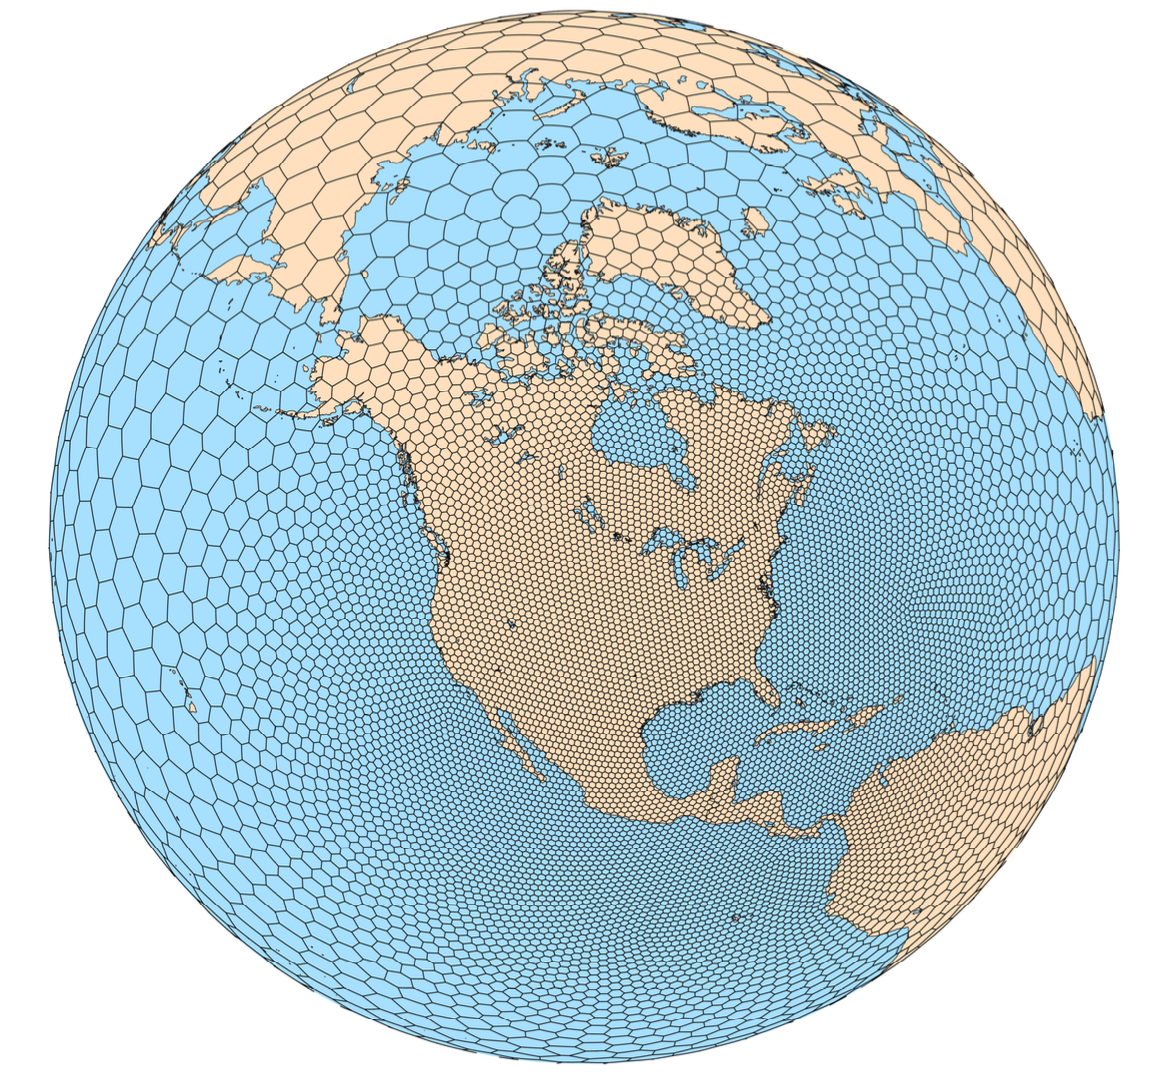
\includegraphics[width=\linewidth,height=0.78\textheight,keepaspectratio]{figuras/db9a63c3ec6ce36e04451467847b54fc6ae550ce.png}
\caption{Exemplo de malha global de resolução variável no MPAS, com refinamento gradual sobre a América do Norte. A imagem ilustra a integração de uma região de maior resolução à própria malha esférica global, com transição suave entre células menores, na área refinada, e células maiores, nas demais regiões do domínio. Fonte: adaptado de MPAS Development Team (2026b).}
\label{fig:figura-13}
\end{figure}

Essa grade de resolução variável é resultado do uso de células de Voronoi em uma malha esférica global, onde a malha primária é composta por polígonos de Voronoi, enquanto a malha secundária usando triângulos de Delaunay. Essa organização permite construir grades quase uniformes ou grades com transição gradual de resolução, evitando a descontinuidade abrupta típica de alguns esquemas de aninhamento. Assim, a resolução variável é, portanto, parte da formulação geométrica do modelo e não apenas um recurso externo de pós-processamento ou de interpolação (Skamarock et al., 2012; Ringler et al., 2011).

\begin{figure}[H]
\centering
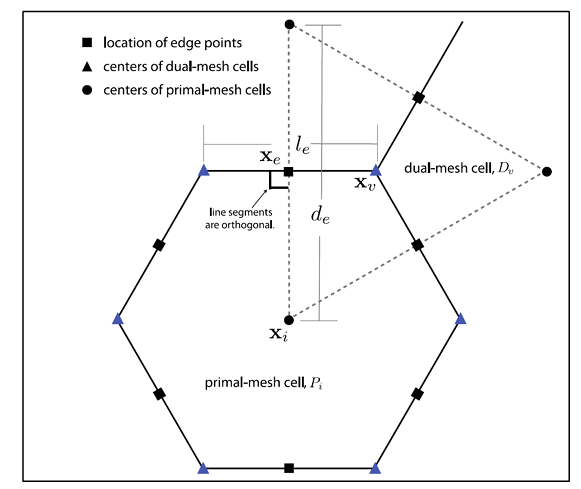
\includegraphics[width=\linewidth,height=0.78\textheight,keepaspectratio]{figuras/e28f57b1db0ac6bfdd5544b8ce0ffe085e99f34f.png}
\caption{Representação esquemática do esquema de duas malhas do MPAS, indicando os centros das células da malha primária (x$_i$), os centros das células da malha dupla (x$_v$) e os pontos de borda nos quais a velocidade é definida (x$_e$). Também são representadas a célula da malha primária (P$_i$), a célula da malha dupla (D$_v$) e os segmentos de linha ortogonais d$_e$ e l$_e$, que correspondem, respectivamente, à distância entre pontos x$_i$ vizinhos e à distância entre pontos x$_v$ vizinhos. Fonte: Sá, 2023.}
\label{fig:figura-14}
\end{figure}

Essa configuração oferece vantagens importantes em relação às grades latitude-longitude tradicionais pois, em grades regulares, a convergência dos meridianos nos polos impõe restrições numéricas e computacionais, frequentemente exigindo filtros ou tratamentos especiais. No MPAS-A, a malha não estruturada distribui as células sobre a esfera de forma mais uniforme ou controladamente variável, o que reduz a dependência de tratamentos específicos nos polos e facilita a construção de domínios globais com refinamento regional (Skamarock et al., 2012; Sá, 2023).

Do ponto de vista da discretização horizontal, o MPAS-A utiliza uma formulação em volumes finitos sobre malhas centroidais de Voronoi, com escalonamento horizontal do tipo C-grid. Nesse arranjo, variáveis escalares, como densidade, temperatura potencial e umidade, são associadas ao centro das células, enquanto o momento horizontal normal às células é definido nas arestas. Essa organização é importante para representar os fluxos entre células vizinhas e para construir operadores diferenciais compatíveis com a geometria não estruturada da malha (Skamarock et al., 2012; Ringler et al., 2010).

O núcleo dinâmico atmosférico do MPAS-A é não hidrostático e totalmente compressível, o que permite sua aplicação em diferentes escalas, desde simulações globais até grades com refinamento regional. Com maior resolução, o modelo consegue representar melhor processos de mesoescala e parte da organização associada à convecção, embora esse desempenho também dependa da configuração física utilizada. Por isso, Skamarock et al. (2012) descrevem o MPAS-A como um modelo multiescala, desenvolvido para atuar entre a escala global e escalas regionais mais refinadas.

Na vertical, o MPAS-A utiliza uma coordenada híbrida associada aos sistemas BTF (basic terrain-following) e STF (smoothed terrain-following). Próximo à superfície, os níveis acompanham a topografia, permitindo representar a influência do relevo na baixa troposfera. Em níveis mais altos, essa influência é suavizada, reduzindo a propagação artificial das irregularidades do terreno para o topo da atmosfera (Skamarock et al., 2012; Sá, 2023; MPAS Development Team, 2026c).

\begin{figure}[H]
\centering
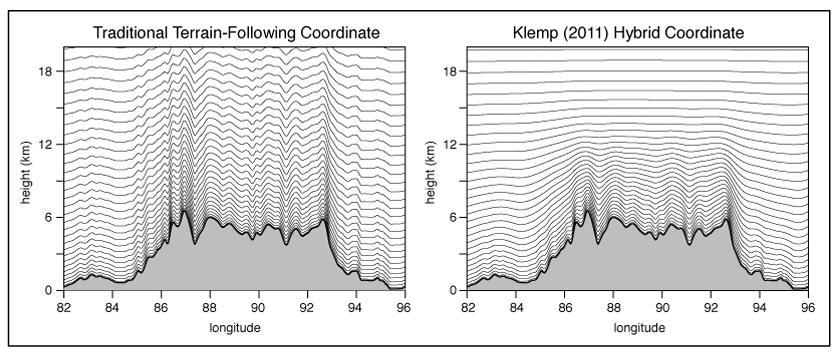
\includegraphics[width=\linewidth,height=0.78\textheight,keepaspectratio]{figuras/5bc7902c7719137833e2d7875c5a80cab66b089d.png}
\caption{Comparação entre a coordenada vertical tradicional do tipo terrain-following e a coordenada híbrida de Klemp (2011), utilizada no MPAS-A. Na coordenada tradicional (BTF), os níveis verticais acompanham a topografia até níveis mais altos, o que representa bem a influência do relevo próximo à superfície, mas pode propagar irregularidades do terreno para a alta troposfera. Na coordenada híbrida BTF/STF, os níveis acompanham melhor o relevo na baixa troposfera e se tornam progressivamente mais suavizados em altitude, reduzindo a influência artificial da topografia nos níveis superiores. Fonte: Sá (2023).}
\label{fig:figura-15}
\end{figure}

A integração temporal do MPAS-A utiliza uma estratégia do tipo split-explicit. Nessa formulação, processos rápidos, como os modos acústicos, são tratados em subpassos menores, enquanto os modos meteorológicos de maior escala avançam com passos de tempo maiores. Com isso, o modelo mantém a estabilidade numérica sem impor o mesmo passo de tempo restritivo a todos os termos das equações, seguindo uma abordagem comum em modelos compressíveis não hidrostáticos (Wicker; Skamarock, 2002; Klemp; Skamarock; Dudhia, 2007; Skamarock et al., 2012).

A preparação de simulações reais no MPAS-A envolve uma sequência específica de arquivos e etapas. A malha é definida no arquivo GRID; as informações estáticas, como topografia, uso e cobertura do solo e demais campos geográficos, são incorporadas no arquivo STATIC; as condições atmosféricas iniciais são interpoladas para a malha e para os níveis verticais no arquivo INIT; e a temperatura da superfície do mar e o gelo marinho podem ser atualizados por um arquivo ou stream específico de SST. Esse fluxo é descrito tanto na documentação oficial quanto em aplicações metodológicas do modelo (MPAS Tutorial Team, 2024; MPAS Development Team, 2026c; Sá, 2023).

\begin{figure}[H]
\centering
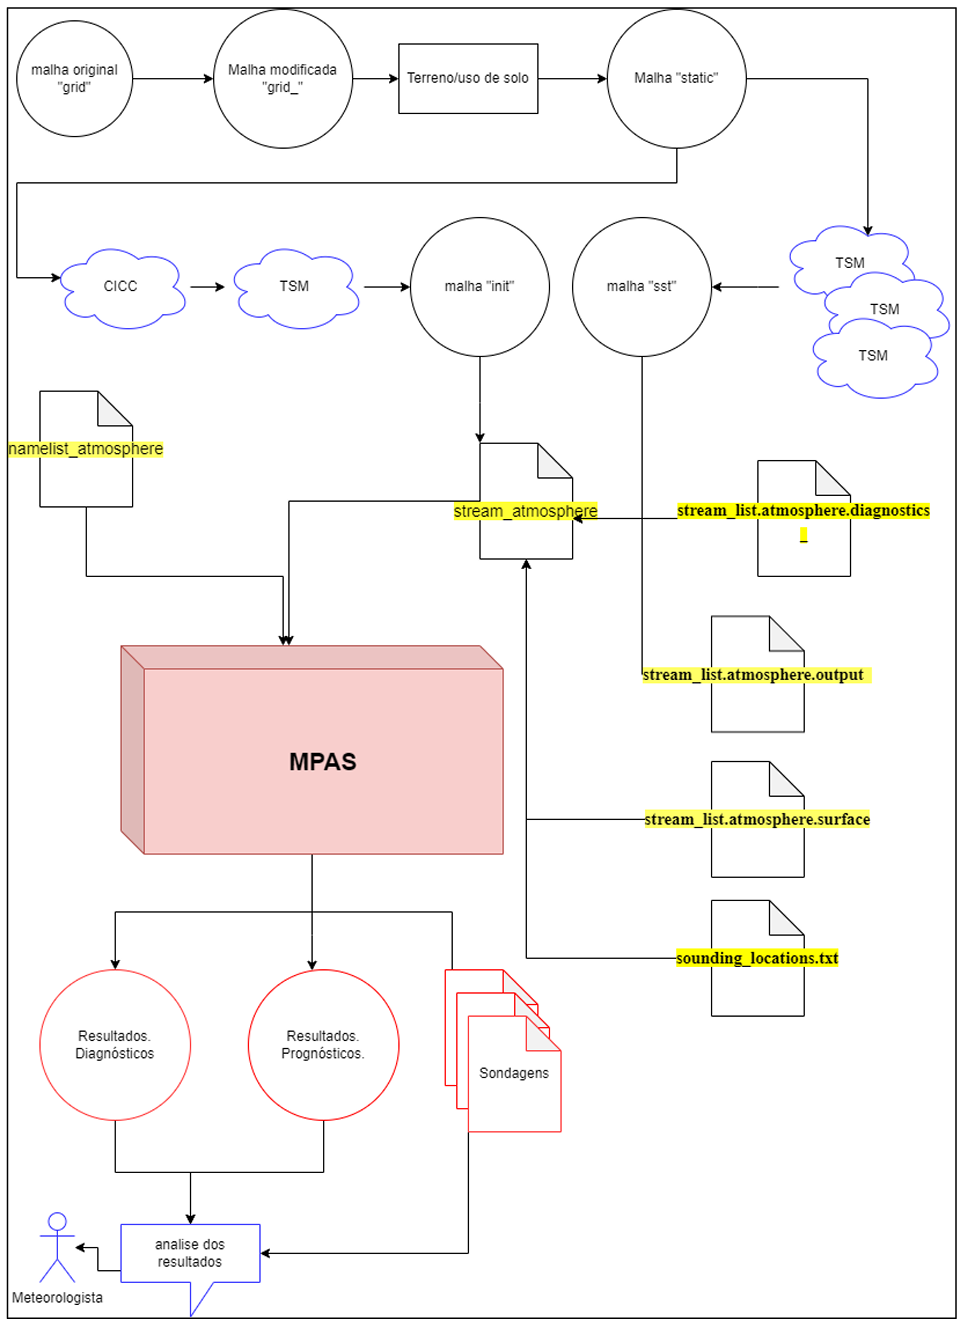
\includegraphics[width=\linewidth,height=0.78\textheight,keepaspectratio]{figuras/551cbf3523b103ecf46379c1e169c03e7cdf4dd6.png}
\caption{Fluxo de preparação e execução do MPAS-A em simulações reais. Fonte: Sá (2023).}
\label{fig:figura-16}
\end{figure}

Em aplicações de previsão com o MPAS-A, as condições iniciais podem ser obtidas a partir de análises, reanálises ou previsões globais, como GDAS/GFS, ERA/ECMWF ou bases equivalentes, conforme o objetivo do experimento e a disponibilidade dos dados. Esses campos definem o estado inicial das variáveis do modelo e, por isso, influenciam diretamente a evolução simulada. Além disso, a temperatura da superfície do mar (TSM) possui um papel específico no fluxo de execução do MPAS, pois pode ser atualizada separadamente das condições atmosféricas iniciais. Nos experimentos de Sá (2023), por exemplo, a base OISST v2.1 foi utilizada para avaliar a sensibilidade das simulações à frequência de atualização da TSM. Dessa forma, foi possível investigar o efeito de diferentes frequências de atualização oceânica sobre a precipitação simulada, sem alterar necessariamente a malha ou o conjunto principal de condições atmosféricas iniciais (Sá, 2023).

A física atmosférica do MPAS-A é organizada em pacotes ou suites, que reúnem parametrizações para processos não resolvidos explicitamente pela grade. A documentação oficial lista opções para convecção, microfísica, radiação, superfície terrestre, camada superficial, camada limite planetária, fração de nuvens e arrasto por ondas de gravidade. Entre as opções convectivas, aparecem esquemas como Tiedtke, New Tiedtke, Grell-Freitas modificada e Kain-Fritsch, já para microfísica, existem opções como WSM 6-class, Thompson e Kessler, equanto para superfície e camada limite há combinações com Noah, Monin-Obukhov, YSU e MYNN, entre outras possibilidades (MPAS Development Team, 2026c; Sá, 2023).

Desses pacotes físicos, dois são particularmente relevantes para aplicações atmosféricas em diferentes escalas: o mesoscale\_reference, que é direcionado a resoluções de mesoescala, onde a convecção profunda ainda precisa ser parametrizada de modo mais tradicional. E o convection\_permitting que é indicado para grades mais finas, próximas da escala em que parte da convecção passa a ser resolvida explicitamente pela dinâmica do modelo. Essa distinção é importante porque o aumento de resolução altera a relação entre precipitação resolvida em grade e precipitação parametrizada, o que pode mudar consideravelmente o comportamento do modelo. (Fowler et al., 2016; Grell; Freitas, 2014; MPAS Development Team, 2026c; Sá, 2023).

O uso do MPAS em previsão operacional ou quase operacional depende ainda da integração com sistemas de assimilação de dados, workflows automatizados e capacidade computacional. Liu et al. (2022) apresentaram o JEDI-MPAS 1.0.0, com implementação e avaliação de EnVar, enquanto Guerrette et al. (2023) avançaram essa linha com o JEDI-MPAS 2.0.0-beta e assimilação ensemble 3DEnVar integrada ao MPAS-Workflow. Esses estudos indicam que o MPAS-A tem avançado em direção a uma infraestrutura compatível com sistemas modernos de previsão, embora a passagem de pesquisa para uso operacional dependa de estabilidade, automação, custo computacional e validação sistemática (Liu et al., 2022; Guerrette et al., 2023).

O custo computacional é uma limitação recorrente em aplicações de alta resolução. Heinzeller, Duda e Kunstmann (2016) avaliaram a escalabilidade do MPAS v3.1 em experimentos globais com altas resoluções (compatíveis com convecção explícita) e mostraram que o modelo pode escalar em ambientes de HPC, mas com exigência significativa de processamento e armazenamento. Sá (2023) também relata elevado custo computacional em experimentos com região refinada a 3 km, especialmente quando as saídas são frequentes. Assim, a vantagem de concentrar resolução sobre uma área de interesse, embora diminua, não elimina o alto custo computacional característico de modelagens numéricas de tempo, e a consequente necessidade de infraestrutura computacional adequada (Heinzeller; Duda; Kunstmann, 2016; Sá, 2023).

Em avaliações idealizadas, Hagos et al. (2013) compararam o MPAS-A e o WRF em simulações de aquaplaneta, com foco nas características de erro associadas a duas estratégias de refinamento: resolução variável global e aninhamento regional. Os autores indicaram que ambas as abordagens apresentam erros ligados à transição de resolução, mas que a estrutura global de resolução variável do MPAS oferece uma alternativa promissora para estudos regionais de clima. Park, Klemp e Skamarock (2014), em simulações idealizadas de onda baroclínica, compararam o refinamento contínuo do MPAS-A com mudanças abruptas de resolução em grades aninhadas do WRF-ARW, mostrando que as malhas de Voronoi do MPAS tendem a produzir transições mais suaves entre resoluções (Hagos et al., 2013; Park; Klemp; Skamarock, 2014).

Em simulações climáticas de alta resolução, Michaelis, Lackmann e Robinson (2019) avaliaram o MPAS-A v5.1 para o Hemisfério Norte, considerando circulação, storm tracks, precipitação e ciclones tropicais. O estudo mostrou que o modelo reproduz vários aspectos de grande escala, mas ainda apresenta vieses regionais e sazonais, especialmente em precipitação. Liang et al. (2021), ao avaliar precipitação sobre o Leste Asiático com CAM-MPAS de resolução variável, também indicaram que a resolução regional refinada pode melhorar a representação de padrões espaciais, mas que os resultados continuam dependentes da física e da configuração adotada (Michaelis; Lackmann; Robinson, 2019; Liang et al., 2021).

Em eventos de precipitação extrema, Zhao et al. (2019) avaliaram o MPASv5.2 sobre o Leste da China e discutiram os impactos combinados de resolução e física, mostrando que o aumento de resolução pode melhorar a representação de precipitação intensa e de estruturas espaciais associadas, mas também ressaltando que a física empregada altera de forma significativa o resultado. Essa conclusão é consistente com outros estudos que tratam da convecção no MPAS: a resolução mais fina tende a ampliar a precipitação resolvida em grade, mas não garante, por si só, a correta intensidade, localização ou evolução temporal dos máximos de chuva (Fowler et al., 2016; Zhao et al., 2019).

A simulação de sistemas convectivos de mesoescala (SCM ou MCS) permanece um desafio. Feng et al. (2021) desenvolveram uma abordagem orientada por processos para avaliar MCS em simulações climáticas e aplicaram o método a configurações de MPAS-CAM com resolução refinada sobre a América do Norte. Os resultados indicaram subestimação do número de MCS e da precipitação associada, além de problemas na variação diurna, duração e intensidade dos sistemas. Esse resultado reforça que, mesmo com resolução refinada em relação a modelos climáticos globais tradicionais, configurações com espaçamento horizontal da ordem de dezenas de quilômetros ainda não são necessariamente suficientes para representar adequadamente a organização convectiva, o ciclo diurno e a precipitação extrema associada a SCM, pois parte importante dos processos convectivos ainda permanece parametrizada. (Feng et al., 2021).

Em ciclones tropicais, Lui et al. (2021) compararam MPAS-A e WRF na previsão e simulação de trajetórias e intensidades no Pacífico Noroeste. Os resultados indicaram desempenho comparável entre os modelos e, em alguns casos, ligeira vantagem do MPAS-A nas trajetórias, mas também apontaram subestimação de intensidade e sensibilidade à inicialização e à resolução. Portanto, mesmo em fenômenos de grande impacto, a estrutura global refinada do MPAS não elimina a necessidade de avaliar separadamente trajetória, intensidade, precipitação e dependência das condições iniciais (Lui et al., 2021).

Além da meteorologia dinâmica, o MPAS também tem sido avaliado em aplicações de qualidade do ar. Gilliam et al. (2021) analisaram a adequação do modelo para simulações retrospectivas globais de qualidade do ar, indicando que sua estrutura pode ser aplicada a estudos atmosféricos que exigem representação consistente de transporte, meteorologia e do acoplamento com processos químicos. Essa aplicação amplia o uso do MPAS para além da previsão de tempo, ainda que seu desempenho continue condicionado à qualidade da meteorologia simulada, à resolução adotada e à representação dos processos subgrade (Gilliam et al., 2021).

Nos experimentos brasileiros de Sá (2023), o modelo foi aplicado em três frentes principais. A primeira avaliou a influência da frequência de inclusão da TSM em previsões de médio prazo para diferentes regiões hidrográficas do Brasil. A segunda analisou o efeito de diferentes estruturas de malha e resoluções em previsão de curto prazo. A terceira aplicou o MPAS em situação de nowcasting para a Região Serrana do Rio de Janeiro. Em conjunto, esses experimentos indicam que o modelo é versátil para aplicações nacionais, mas que seu desempenho depende da coerência entre configuração da malha, pacote físico, condições iniciais, atualização de TSM e fenômeno de interesse (Sá, 2023).

A revisão dos estudos supracitados indica que o MPAS-A possui vantagens conceituais claras para aplicações multiescala, especialmente por permitir refinamento regional dentro de um domínio global, evitar fronteiras laterais internas e usar uma formulação dinâmica compatível com malhas não estruturadas. No entanto, essas vantagens não significam superioridade automática em todas as aplicações. O desempenho depende da resolução, da física, da inicialização, da atualização da TSM, do tempo de integração, do fenômeno analisado e da base de verificação. Em precipitação intensa, por exemplo, os estudos mostram que ainda podem ocorrer erros de localização, subestimativa de máximos, suavização espacial e deficiências no ciclo diurno da convecção (Fowler et al., 2016; Zhao et al., 2019; Feng et al., 2021; Sá, 2023).

Assim, o MPAS-A representa, de forma geral, uma alternativa relevante aos modelos globais tradicionais e aos modelos regionais aninhados, pois combina domínio global, malha não estruturada, resolução variável, núcleo não hidrostático compressível e pacotes físicos adaptáveis a diferentes escalas. Essa combinação permite investigar fenômenos atmosféricos em que processos locais e circulação de grande escala estão fortemente conectados, mas ainda assim, sua utilização em previsão de tempo, simulações climáticas ou estudos de eventos extremos devem ser acompanhadas por avaliações específicas para cada região, período e variável, especialmente quando o objetivo é analisar precipitação intensa, convecção organizada ou impactos de resolução. Portanto, o MPAS-A deve ser entendido como uma ferramenta multiescala promissora e tecnicamente robusta, mas assim como muitas outras, sensível às escolhas de configuração e às limitações comuns à modelagem atmosférica numérica.

Especialmente no contexto brasileiro, essa relevância é reforçada pelo MONAN, que utiliza o MPAS como base do componente atmosférico, o tornando base para uma plataforma comunitária nacional de previsão, pesquisa e desenvolvimento físico-computacional.

\chapter{Lacuna e contribuição do trabalho}

A revisão bibliográfica apresentada indica que o MPAS-A possui potencial para aplicações multiescala, especialmente por combinar domínio global, malha não estruturada e possibilidade de refinamento regional contínuo. Estudos anteriores avaliaram o modelo em experimentos idealizados, simulações climáticas, eventos de precipitação intensa, sistemas convectivos de mesoescala, ciclones tropicais e aplicações nacionais, mostrando vantagens associadas à resolução variável, mas também limitações relacionadas à física empregada, à inicialização, ao custo computacional e à representação de extremos de precipitação (Hagos et al., 2013; Park; Klemp; Skamarock, 2014; Zhao et al., 2019; Feng et al., 2021; Lui et al., 2021; Sá, 2023).

Embora existam estudos avaliando modelos numéricos em eventos de chuva intensa no Brasil, ainda existe uma lacuna de avaliações que comparem diretamente o MPAS-A com modelos regionais já consolidados no contexto nacional, como o ETA e o BRAMS. Essa comparação é relevante porque o MPAS-A adota uma estratégia distinta, com domínio global e refinamento regional incorporado à própria malha, enquanto ETA e BRAMS seguem a lógica de modelos regionais de área limitada. Além disso, a entrada do MPAS-A como base do componente atmosférico do MONAN reforça a necessidade de avaliar, no contexto brasileiro, em que medida essa abordagem pode trazer ganhos efetivos na representação de eventos extremos de precipitação.

No caso do evento de abril-maio de 2024 no Rio Grande do Sul, essa lacuna se torna particularmente pertinente, pois a precipitação extrema foi resultado da combinação entre anomalias de grande escala, jato de baixos níveis, frentes frias, transporte de umidade e sistemas convectivos de mesoescala (Reboita et al., 2024). Assim, esse passa ser um caso adequado para avaliar a capacidade do modelo em representar um evento em que processos locais e de grande escala estiveram fortemente acoplados.

Nesse sentido, este trabalho contribui ao avaliar simulações de curto prazo do MPAS-A para o evento extremo de precipitação ocorrido no Rio Grande do Sul entre abril e maio de 2024, considerando diferentes configurações de resolução espacial e comparando seus resultados com os modelos ETA e BRAMS. Com isso, busca-se analisar não apenas a capacidade do modelo em representar os acumulados de precipitação, mas também sua habilidade em reproduzir a distribuição espacial, a intensidade e o deslocamento dos principais núcleos de chuva. Essa avaliação permite discutir, de forma aplicada, as potencialidades e limitações do MPAS-A para eventos extremos no Sul do Brasil e fornece uma base para estudos futuros envolvendo sua utilização em previsão de tempo e modelagem atmosférica no contexto nacional.

\chapter{Metodologia}

\section{Dados de Validação de precipitação.}

Para avaliar a qualidade das previsões de precipitação geradas pelos modelos atmosféricos utilizados neste estudo, adotou-se como referência observacional o produto de precipitação em grade MERGE, operacionalmente disponibilizado pelo Centro de Previsão de Tempo e Estudos Climáticos (CPTEC) do Instituto Nacional de Pesquisas Espaciais (INPE).

O MERGE (Rozante et al., 2010) é um conjunto de dados de alta resolução espacial desenvolvido reduzir as incertezas associadas à interpolação de precipitação em regiões caracterizadas por redes pluviométricas irregulares ou pouco densas especificamente para a América do Sul.

O método de construção do MERGE envolve uma sequência estruturada de procedimentos: Inicialmente, os dados pluviométricos de superfície são georreferenciados para a mesma grade espacial das estimativas de satélite, assegurando compatibilidade entre as duas fontes de informação. Em seguida, remove-se um bloco de 5 $\times$ 5 pixels do IMERG ao redor de cada estação, impedindo que a estimativa satelital interfira na região de influência direta da medição terrestre. Após essa etapa, é criada uma lista combinada contendo primeiramente todas as observações de superfície e, em seguida, os valores satelitais remanescentes. A interpolação espacial do campo final de precipitação é realizada por meio da técnica de Análise Objetiva de Barnes, que aplica correções sucessivas ponderadas pela distância das observações, utilizando parâmetros como o raio de influência e o coeficiente de convergência para determinar a suavização adequada do campo (Rozante et al., 2010).

Atualmente, o produto cobre toda a América do Sul e parte dos oceanos próximos, possui resolução espacial de 0,1$^\circ$ $\times$ 0,1$^\circ$ (aproximadamente 11 km) e disponibiliza uma série temporal contínua desde junho de 2000, que é disponibilizada em acumulados diários (entre 12Z do dia anterior e 12Z do dia corrente) ou em acumulados horários.

Os dados do MERGE encontram-se disponíveis em formato GRIB2 e podem ser obtidos por download direto via FTP no endereço: \textcolor{red}{\url{https://ftp.cptec.inpe.br/modelos/tempo/MERGE/GPM/}}.

Como as previsões dos modelos utilizados neste estudo foram produzidas em formato horário e referenciadas temporalmente em UTC±0, optou-se pela utilização dos dados horários do MERGE, com posterior acumulação das 24 horas de cada dia, garantindo a equivalência temporal dos períodos de acumulação de precipitação entre todas as fontes analisadas.

É importante destacar que, embora apresente desempenho superior à simples interpolação dos valores de pluviômetros, o MERGE, assim como outros produtos gridados de precipitação que utilizam imagens de satélite e estações in-situ, ainda apresenta degradação em sua precisão em áreas com baixa densidade de estações (Rozante et al. (2024); Silva et al. (2020)).

Por essa razão, optou-se por validar previamente a acurácia espacial e temporal do produto para a região e o período de interesse, antes de utilizá-lo como referência observacional na comparação com as previsões numéricas.

Para essa validação, foram utilizadas estações meteorológicas automáticas com registros horários de precipitação, disponibilizadas pelo Instituto Nacional de Meteorologia (INMET). O catálogo completo das estações automáticas no Brasil encontra-se disponível no endereço: \textcolor{red}{\url{https://portal.inmet.gov.br/paginas/catalogoaut}}, enquanto os dados históricos anuais podem ser acessados em \textcolor{red}{\url{https://portal.inmet.gov.br/dadoshistoricos}}.

Para este estudo, foram selecionadas todas as estações localizadas geograficamente dentro do estado do Rio Grande do Sul que apresentavam séries completas de precipitação horária entre os dias 28/04/2024 e 03/05/2024, garantindo assim uma base observacional confiável para todo o evento analisado.

Para validar espacialmente os campos de precipitação do produto MERGE, foram elaborados gráficos de ``heatmaps'' em comparação com os dados das estações automáticas da região. Essa análise permitiu verificar se os padrões espaciais de chuva representados pelo MERGE estavam coerentes com aqueles observados nas estações, conforme ilustrado na \textcolor{red}{Figura X}.

\begin{figure}[H]
\centering
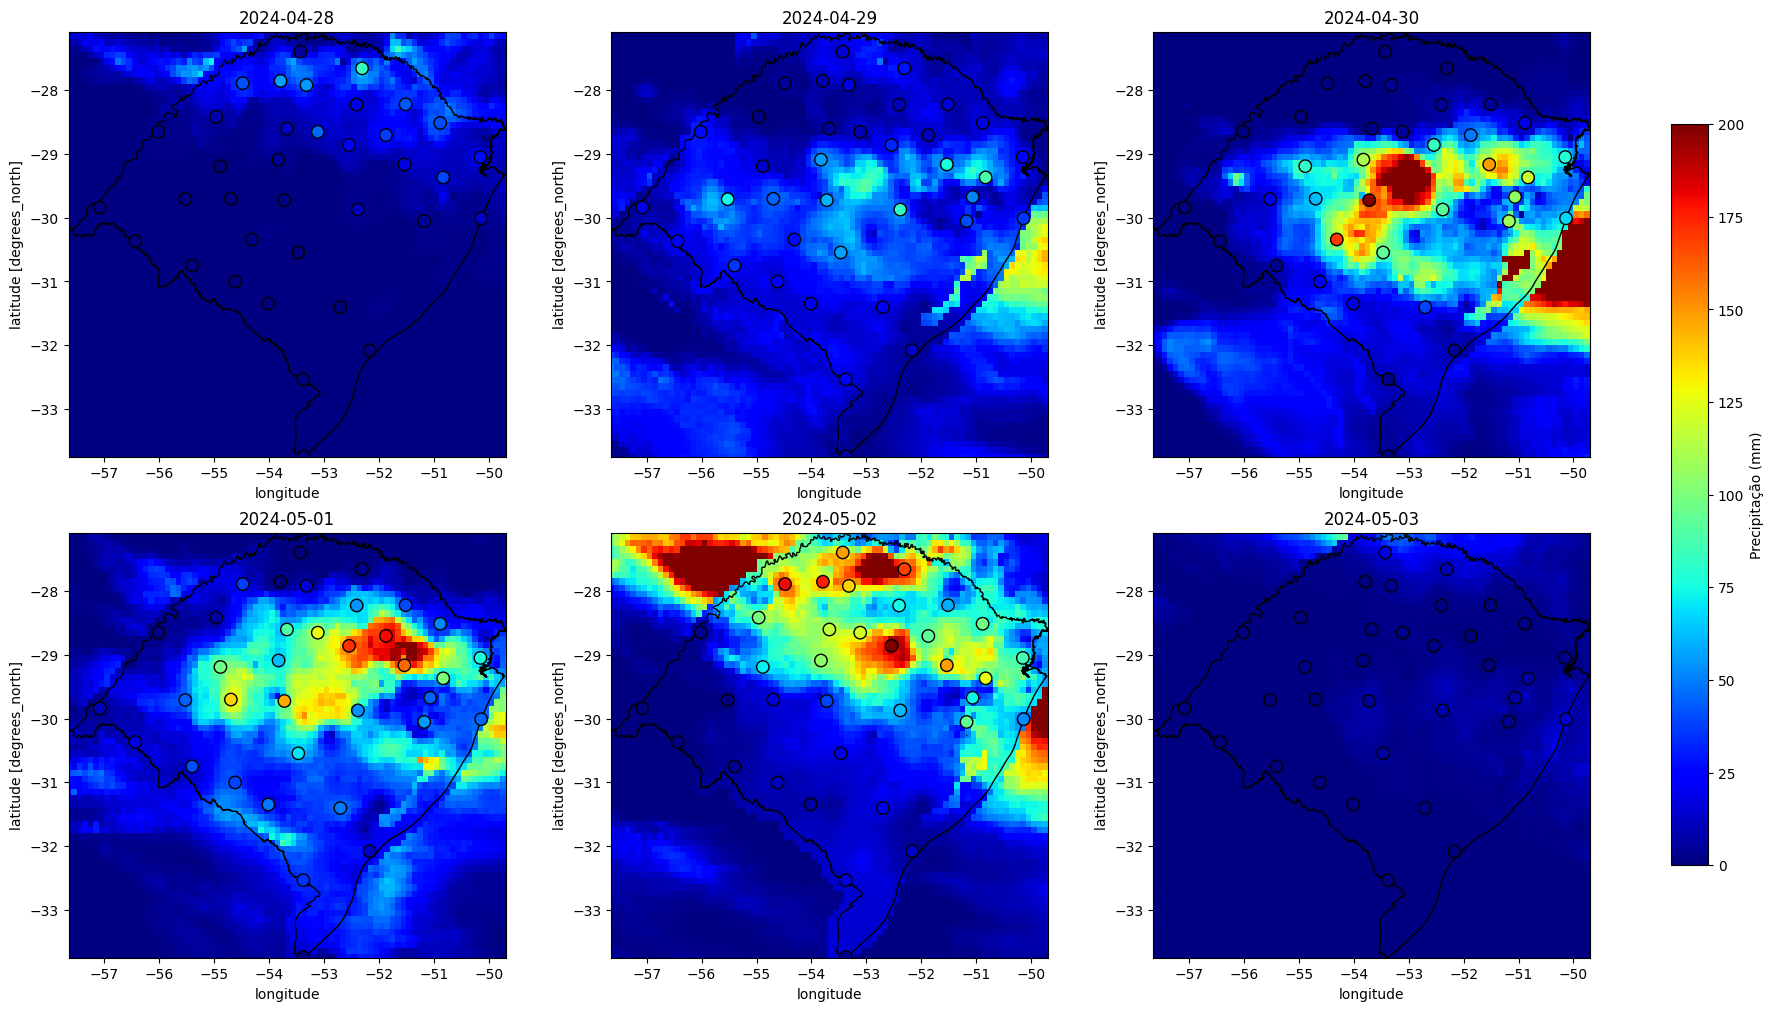
\includegraphics[width=\linewidth,height=0.78\textheight,keepaspectratio]{figuras/6aa03e456657a743593f67366d03e3efc3a8457e.png}
\caption{\textcolor{red}{Inserir legenda da figura.}}
\label{fig:figura-17}
\end{figure}

Observou-se, portanto, que o produto MERGE representou de forma consistente tanto os valores quanto a distribuição espacial da precipitação sobre o continente. Identificaram-se apenas discrepâncias localizadas, sobretudo na região da Lagoa dos Patos, onde o MERGE apresentou volumes substancialmente superiores aos registrados pelas estações próximas durante os dias de maior precipitação. Padrões semelhantes também foram verificados em áreas da Argentina e sobre o oceano Atlântico nas datas de 30/04/2024 e 02/05/2024, o que era esperado diante da ausência de estações nessas regiões para ancorar a interpolação. Apesar dessas limitações pontuais e, como o foco deste trabalho está concentrado na análise da precipitação no estado do Rio Grande do Sul, o produto foi considerado adequado para utilização como referência observacional.

Adicionalmente, com o objetivo de avaliar temporalmente a correspondência entre o observado nas estações e o representado pelo MERGE, optou-se pela elaboração de gráficos de boxplot contendo os valores de correlação de Pearson e de RMSE calculados para as 32 estações selecionadas, conforme apresentado na \textbf{\textcolor{red}{Figura X}}. Essas métricas foram obtidas a partir dos acumulados diários de precipitação tanto das estações quanto do pixel mais próximo de cada estação no produto em grade ao longo do período estudado.

\begin{figure}[H]
\centering
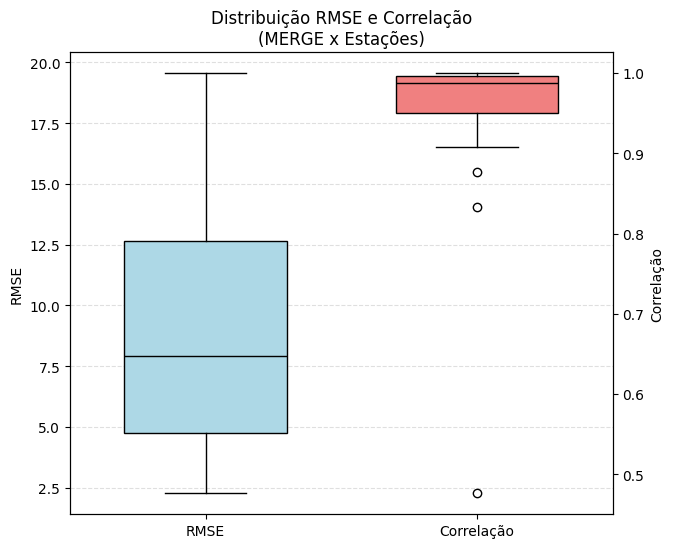
\includegraphics[width=\linewidth,height=0.78\textheight,keepaspectratio]{figuras/87d83573f3a6ef9ee923b024adb08611acd0a412.png}
\caption{\textcolor{red}{Inserir legenda da figura.}}
\label{fig:figura-18}
\end{figure}

Pode-se observar na \textcolor{red}{Figura X} que mais de 90\% das estações apresentam coeficientes de correlação de Pearson superiores a 0.9, evidenciando uma elevada concordância temporal entre o MERGE e os dados observados. Quando esse resultado é combinado com os baixos valores de RMSE (com aproximadamente 75\% das estações apresentando erros inferiores a 12,5 mm) reforça-se a conclusão de que há, de fato, uma alta consistência temporal entre as séries de precipitação registradas pelas estações e aquelas representadas pelo produto MERGE.

Em vista dos resultados apresentados (\textcolor{red}{figura X e X}) optou-se, com maior segurança quanto à qualidade da representação do evento, por utilizar o produto MERGE como ground truth da precipitação a ser comparada com as previsões numéricas obtidas.

\section{Dados de Precipitação Prevista}

\subsection{Organização Geral dos experimentos}

Com o objetivo de analisar a sensibilidade dos modelos ETA, BRAMS e MPAS em relação à variação na data de inicialização das simulações, este estudo foi estruturado em dois experimentos independentes. Tendo sido, em ambos, utilizados os mesmos parâmetros, configurações e resoluções espaciais, garantindo a condição inicial empregada em cada simulação como única diferença entre os experimentos.

O objetivo desta abordagem é analisar a influência da proximidade temporal entre a condição inicial e o pico de precipitação do evento meteorológico estudado, verificando a hipótese de que, para este caso, condições iniciais mais próximas aos maiores acumulados poderiam proporcionar melhorias na qualidade preditiva dos modelos para este evento específico.

Um resumo das principais características de cada experimento é apresentado nas \textcolor{red}{Tabelas X e Y.}

\begin{figure}[H]
\centering
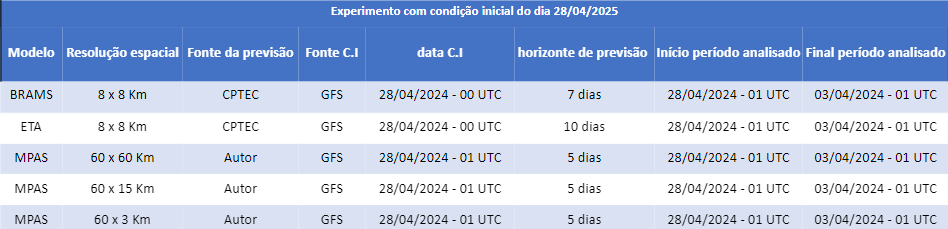
\includegraphics[width=\linewidth,height=0.78\textheight,keepaspectratio]{figuras/7b3aa9221d228e7a6c0a841ef97da97916f7b8d0.png}
\caption{\textcolor{red}{Inserir legenda da figura.}}
\label{fig:figura-19}
\end{figure}

\begin{figure}[H]
\centering
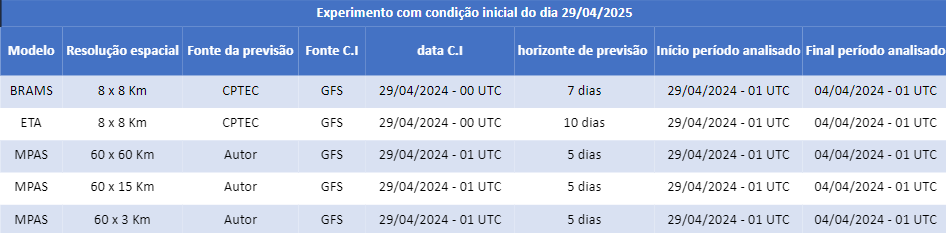
\includegraphics[width=\linewidth,height=0.78\textheight,keepaspectratio]{figuras/e8306f130b19152d19798c1df006e0bdd1d29779.png}
\caption{\textcolor{red}{Inserir legenda da figura.}}
\label{fig:figura-20}
\end{figure}

\subsection{Obtenção dos dados do ETA e BRAMS}

Os dados de previsão histórica empregados neste estudo como previsões de referência, foram obtidos a partir dos modelos numéricos ETA e BRAMS, ambos com resolução espacial aproximada de 8 km. Essas previsões foram utilizadas para fins de comparação com os resultados gerados pelo modelo MPAS.

O modelo ETA encontra-se em operação no Centro de Previsão de Tempo e Estudos Climáticos (CPTEC/INPE) desde 1996, cobrindo grande parte da América do Sul. Esse modelo fornece previsões detalhadas de variáveis meteorológicas e é amplamente utilizado tanto em previsões de curto prazo, com horizontes de até 15 dias, quanto em aplicações sazonais, incluindo previsão de precipitação, monitoramento de eventos extremos e suporte a atividades agrícolas e hidrológicas (CHOU \emph{et al}., 2020; MACHADO \emph{et al}., 2007).

O modelo BRAMS, por sua vez, foi desenvolvido a partir do Regional Atmospheric Modeling System (RAMS) e posteriormente adaptado para representar de forma mais adequada as condições atmosféricas tropicais, em especial sobre o território brasileiro. Atualmente, o BRAMS é utilizado operacionalmente no CPTEC/INPE e em diversos centros regionais, fornecendo previsões de tempo e de qualidade do ar em alta resolução espacial para o Brasil e para a América do Sul (FREITAS \emph{et al}., 2016; MORAES \emph{et al}., 2013).

Ambos os modelos desempenham papel central na emissão de alertas meteorológicos e no apoio à tomada de decisão em setores altamente sensíveis às condições climáticas, como agricultura, recursos hídricos e defesa civil. A utilização contínua desses sistemas por mais de duas décadas em âmbito nacional fundamenta a escolha do ETA e do BRAMS como padrões de referência para a avaliação das previsões associadas ao evento analisado neste trabalho.

A obtenção dos dados foi realizada por meio do DataServer institucional do INPE \textsuperscript{{[}27{]}}. Esse repositório centraliza, além de outros dados, as previsões operacionais e históricas dos principais modelos numéricos executados pelo CPTEC, organizando os arquivos de forma sistemática em diretórios hierárquicos que contemplam o modelo, a resolução espacial, o ano, o mês, o dia e o horário de início da simulação. As previsões históricas dos modelos ETA e BRAMS encontram-se especificamente no diretório denominado ``dataserver\_modelos'', permitindo o acesso direto aos campos previstos para diferentes datas e horários de inicialização.

Os dados são disponibilizados em arquivos individuais no formato GRIB2, com resolução temporal horária. Cada arquivo contém o conjunto completo de variáveis atmosféricas previstas pelos respectivos modelos para um intervalo de uma hora, incluindo variáveis dinâmicas, termodinâmicas e de superfície. Esse formato é amplamente utilizado para armazenar resultados de modelagem numérica de tempo e clima, por ser eficiente no armazenamento e distribuição de grandes volumes de dados meteorológicos (GLAHN; LAWRENCE, 2002).

No que se refere à variável de precipitação, é importante destacar que históricos de previsão disponibilizados para os modelos ETA e BRAMS apresentam diferenças na forma como essa variável é disponibilizada. No caso do modelo ETA, foi utilizada a variável de precipitação total, a qual já é fornecida diretamente como o acumulado correspondente ao intervalo de uma hora representado por cada arquivo. Dessa forma, não foi necessário nenhum processamento adicional para obtenção da precipitação horária.

Por outro lado, no modelo BRAMS, a precipitação total não é disponibilizada como uma variável única. Em vez disso, o modelo fornece separadamente os campos de precipitação convectiva e precipitação não convectiva, ambos acumulados desde o início da simulação. Assim, para tornar os dados compatíveis com a análise horária proposta neste trabalho, foi necessário realizar um procedimento de desacumulação temporal, no qual a precipitação horária foi obtida pela diferença entre os acumulados sucessivos, somando-se posteriormente as componentes convectiva e não convectiva. Esse procedimento é comum em estudos que utilizam saídas do BRAMS e outros modelos atmosféricos que trabalham com variáveis acumuladas no tempo e, no caso deste estudo, foi feito por meio de um script em linguagem Python.

Para as datas de interesse deste estudo, correspondentes aos dias 28 e 29 de abril de 2024, apenas as previsões com horário inicial de 00 UTC estavam disponíveis no DataServer do CPTEC. Em ambos os modelos, as simulações foram inicializadas a partir das condições iniciais fornecidas pelo Global Forecast System (GFS), modelo global operacional do National Centers for Environmental Prediction (NCEP), amplamente utilizado como fonte de condições iniciais e de contorno para modelos regionais (NOAA, 2025).

As análises iniciais do GFS utilizadas nessas simulações estavam disponíveis no repositório operacional NOMADS (NOAA Operational Model Archive and Distribution System)\textsuperscript{{[}30{]}}. Esse sistema disponibiliza as análises e previsões do GFS com um histórico de até aproximadamente dez dias anteriores à data corrente.

Dessa forma, os dados de previsão operacional do modelo BRAMS com resolução de 8 km, inicializados às 00 UTC dos dois dias de interesse, foram obtidos a partir dos seguintes endereços eletrônicos:

\url{https://dataserver.cptec.inpe.br/dataserver_modelos/brams/ams_08km/brutos/2024/04/28/00/}

\url{https://dataserver.cptec.inpe.br/dataserver_modelos/brams/ams_08km/brutos/2024/04/29/00/}

De maneira análoga, os dados de previsão operacional do modelo ETA com resolução de 8 km, também inicializados às 00 UTC dos dias 28 e 29 de abril de 2024, foram obtidos a partir dos seguintes diretórios:

\url{https://dataserver.cptec.inpe.br/dataserver\_modelos/eta/ams\_08km/brutos/2024/04/28/00/}

\url{https://dataserver.cptec.inpe.br/dataserver_modelos/eta/ams_08km/brutos/2024/04/29/00/}

Os conjuntos de dados obtidos a partir desses repositórios constituem a base das análises comparativas realizadas neste trabalho, permitindo a avaliação do desempenho dos modelos ETA e BRAMS na representação da precipitação associada ao evento extremo ocorrido no período de estudo, bem como a sua comparação com os resultados obtidos com o MPAS.

\subsection{Simulações com o MPAS}

\subsubsection{Grades e seus ajustes para a região de estudo}

Conforme \textcolor{red}{descrito na Seção 2.2}, o MPAS emprega uma malha horizontal não estruturada baseada em tesselações esféricas centroidais de Voronoi \textsuperscript{{[}31{]}}, que possibilita a aplicação de refinamento espacial localizado de forma contínua.

Neste trabalho, foram utilizadas três configurações distintas de malha, selecionadas com o objetivo de avaliar a sensibilidade dos resultados do modelo à sua resolução espacial. As configurações consistiram em: uma malha quase uniforme de resolução fixa de 60x60 km, uma malha de resolução variável indo de 60 km até 15 km na área de interesse, e uma malha de resolução variável indo de 60 km até 3 km na área de interesse. Nas malhas de resolução variável, a região refinada é incorporada de forma gradual, mantendo-se uma resolução mais grosseira fora da área de interesse, o que reduz o custo computacional em comparação com malhas uniformemente refinadas.

As malhas arquivos (.grid), bem como seus respectivos arquivos de conectividade (\emph{graph.info}) e, quando disponíveis, os arquivos de campos estáticos (\emph{static.nc}), foram obtidos a partir do repositório oficial do MPAS (\url{https://mpas-dev.github.io/atmosphere/atmosphere_meshes.html}). Para a malha quase uniforme de 60 km, o arquivo \emph{static.nc} foi utilizado diretamente, uma vez que já se encontra previamente interpolado com os campos geográficos padrão. Em contrapartida, para as malhas de resolução variável (60x15 km e 60x3 km), os arquivos \emph{static} não são fornecidos no repositório e foram gerados posteriormente durante a etapa de pré-processamento do modelo.

Uma vez que as malhas de resolução variável disponibilizadas pelo MPAS apresentam, por padrão, a região de refinamento centrada em 0$^\circ$ de latitude e 0$^\circ$ de longitude, foi necessária a realocação espacial da região refinada para que esta coincidisse com a área de interesse do estudo. Para esse fim, utilizou-se o utilitário grid\_rotate, que aplica uma rotação rígida da malha na esfera, preservando sua estrutura e evitando a necessidade de regeneração completa da malha. Um diagrama exemplificando o processo é mostrado \textcolor{red}{na figura x.}

\begin{figure}[H]
\centering
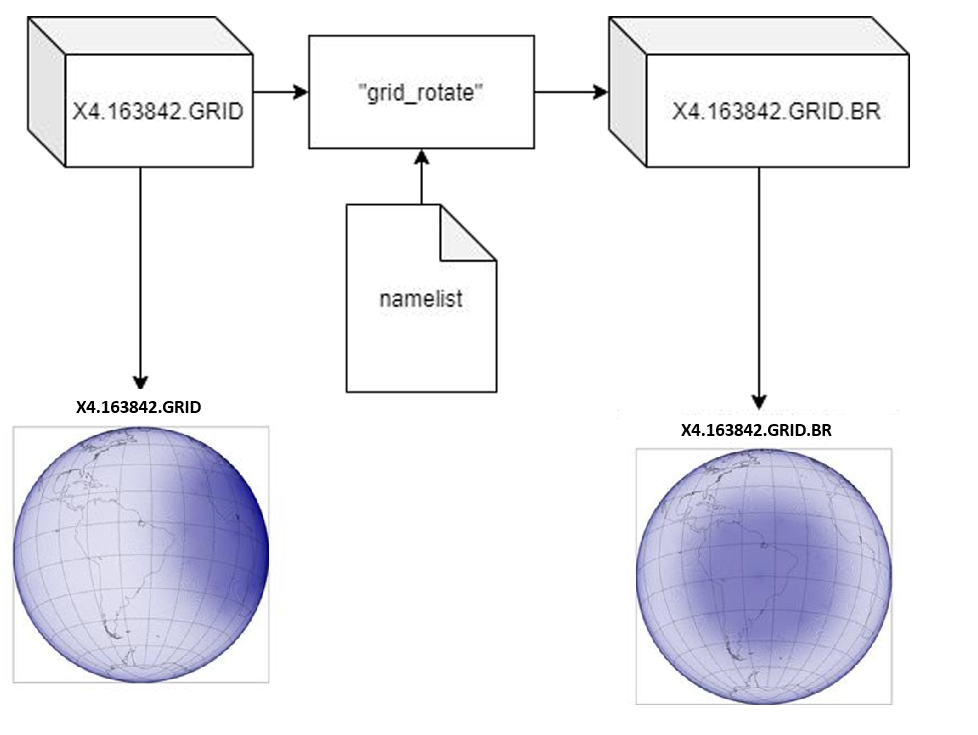
\includegraphics[width=\linewidth,height=0.78\textheight,keepaspectratio]{figuras/2848e07284420ee8f9a28530ca627c4771847722.png}
\caption{\textcolor{red}{Inserir legenda da figura.}}
\label{fig:figura-21}
\end{figure}

Os parâmetros de rotação foram definidos por meio de um arquivo namelist.input, no qual se especificaram as coordenadas geográficas originais e finais do ponto de referência da malha, bem como a rotação adicional em torno do eixo local. Para este estudo a malha foi centrada aproximadamente no centro do estado do Rio Grande do Sul e as configurações do arquivo namelist.input estão descritas \textcolor{red}{na tabela x.}

\begin{figure}[H]
\centering
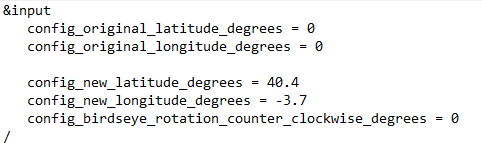
\includegraphics[width=\linewidth,height=0.78\textheight,keepaspectratio]{figuras/f13027b8fa3e4ec0c2df59b4039d24054fb43907.png}
\caption{\textcolor{red}{Inserir legenda da figura.}}
\label{fig:figura-22}
\end{figure}

Após a definição geométrica das malhas, procedeu-se à decomposição paralela necessária para a execução do modelo em múltiplos processadores. Para cada malha, verificou-se inicialmente a disponibilidade de arquivos de particionamento compatíveis com o número de processos MPI empregados nas simulações. Nos casos em que tais arquivos não estavam disponíveis, foram gerados novos arquivos de decomposição (\emph{graph.info.part.N}) a partir do arquivo de conectividade (\emph{graph.info}), utilizando-se a bibliotecas METIS. Esse procedimento garantiu a correspondência entre o número de partições da malha e o número de tarefas MPI utilizadas na execução do modelo.

O comando utilizado para esse fim para cada grade foi:

\emph{\$ gpmetis -minconn -contig -niter=200 ``caminho do arquivo .graph.info'' "número de processadores''}

Dessa forma, a preparação das malhas envolveu, de maneira sistemática, a seleção das resoluções espaciais, a realocação da região de refinamento nas malhas de resolução variável e a geração dos arquivos de decomposição paralela, assegurando consistência geométrica, numérica e computacional para as simulações realizadas com o MPAS.

\subsubsection{Incorporação das informações estáticas na grade de análise}

A incorporação à grade espacial das informações de topografia, uso e cobertura do solo e demais campos geográficos considerados estáticos para a simulação de curto prazo foi realizada por meio da geração do arquivo \emph{static}. Esse arquivo contém os campos estáticos interpolados para a malha espacial do modelo e é requisito fundamental para a execução de simulações com malhas de resolução variável, uma vez que tais arquivos não são disponibilizados previamente no repositório oficial do MPAS.

Para este trabalho, a geração do arquivo \emph{static} foi realizada a partir das malha de resolução variável previamente preparadas e rotacionadas, de forma que a região de maior refinamento espacial estivesse corretamente posicionada sobre a área de interesse. Este processo de interpolação dos campos geográficos foi conduzido \textcolor{red}{}utilizando-se os arquivos estáticos disponíveis no WRF Preprocessing System (WPS) \textsuperscript{{[}32{]}} por intermédio do pré-processador do MPAS, o init\_atmosphere.

Para isso, o arquivo namelist.init\_atmosphere foi ajustado \textcolor{red}{como na tabela X} de modo a ativar apenas os estágios necessários à geração do \emph{static}, com o parâmetro config\_geog\_data\_path sendo configurado para apontar para o diretório com os dados geográficos do WPS, assegurando o acesso correto aos dados de topografia, uso do solo, fração de vegetação, albedo e demais campos necessários.

\begin{figure}[H]
\centering
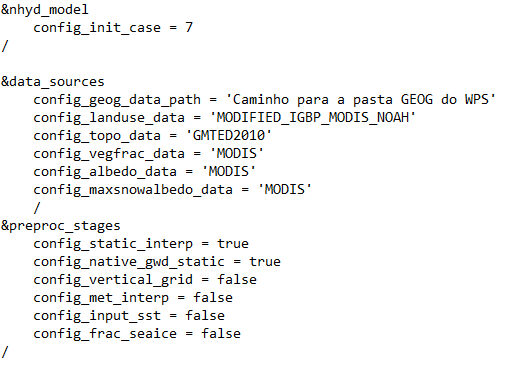
\includegraphics[width=\linewidth,height=0.78\textheight,keepaspectratio]{figuras/ebd24d6449d44c92dc0085e1d0243996fcdc756b.png}
\caption{\textcolor{red}{Inserir legenda da figura.}}
\label{fig:figura-23}
\end{figure}

Paralelamente, o arquivo streams.init\_atmosphere foi configurado para definir explicitamente os arquivos de entrada e saída do pré-processamento. Nesse arquivo o campo de entrada foi especificado (mostrando o exemplo de configuração para a grade de 90x25 km) como x4.163842.RS.grid.nc, correspondente à malha rotacionada, enquanto o campo de saída foi definido como x4.163842.RS.static.nc, que contém os campos estáticos interpolados para a malha MPAS. \textcolor{red}{A tabela x} apresenta o conteúdo do arquivo streams.init\_atmosphere devidamente configurado.

\begin{figure}[H]
\centering
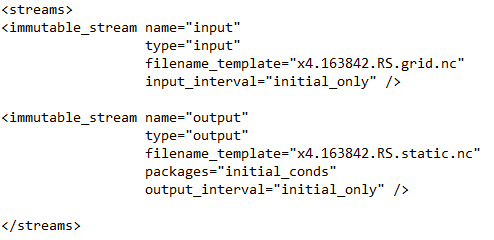
\includegraphics[width=\linewidth,height=0.78\textheight,keepaspectratio]{figuras/ef0ddce24d965a66eb2ef45962cbb8c0c0d8cc37.png}
\caption{\textcolor{red}{Inserir legenda da figura.}}
\label{fig:figura-24}
\end{figure}

Uma vez concluídas as configurações dos arquivos de controle, o pré-processador ``init\_atmosphere'' foi executado e este procedimento resultou na geração do arquivo x4.163842.RS.static.nc, o qual incorpora de forma consistente as informações de topografia, uso e cobertura do solo e demais campos geográficos estáticos necessários à simulação atmosférica.

O fluxo geral desse processo de geração do arquivo \emph{static} foi executado para cada uma das duas malhas de resolução variável para cada experimento, e ele segue o esquema apresentado na \textcolor{red}{figura x}.

\begin{figure}[H]
\centering
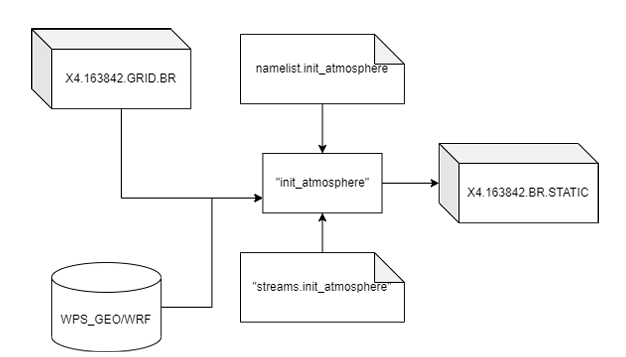
\includegraphics[width=\linewidth,height=0.78\textheight,keepaspectratio]{figuras/9ef85f500a48f3e1e9680e7b8d2db81a64c3c734.png}
\caption{\textcolor{red}{Inserir legenda da figura.}}
\label{fig:figura-25}
\end{figure}

\subsubsection{Dados atmosféricos utilizados como condição inicial}

As simulações foram inicializadas a partir da primeira hora de previsão dos arquivos correspondentes a cada um dos dias de início da simulação (28 e 29 de abril de 2024) do Global Forecast System (GFS), com resolução horizontal de 0,25$^\circ$.

Embora exista o endpoint operacional do GFS/NCEP, disponível em \url{https://nomads.ncep.noaa.gov/pub/data/nccf/com/gfs/prod/}, utilizado para acesso aos campos mais recentes do modelo e empregado pelo INPE nas rodadas operacionais do ETA e do BRAMS, nas simulações realizadas com o MPAS foi necessário utilizar o arquivo histórico do GFS, devido à distância temporal entre o evento e a execução das rodadas. Para isso, foram utilizados os dados do conjunto \emph{NCEP GFS 0.25 Degree Global Forecast Grids Historical Archive}, disponibilizado pelo NCAR/GDEX em \url{https://gdex.ucar.edu/datasets/d084001/}, com acesso direto aos arquivos por meio do endpoint \url{https://osdf1.newy32aoa.nrp.internet2.edu:8443/ncar/gdex/d084001}.

Tanto o endpoint operacional quanto o arquivo histórico correspondem a campos de análise e previsão do GFS operacional, diferindo principalmente quanto à forma de disponibilização e ao objetivo de acesso: operacional e em tempo quase real no primeiro caso, e histórico no segundo. Dessa forma, embora as fontes de acesso sejam distintas, as condições iniciais de atmosfera utilizadas nas simulações do MPAS são iguais aos campos utilizados nas simulações do ETA e BRAMS.

No entanto, o MPAS não consegue utilizar esse arquivo em formato GRIB-2 diretamente como condição inicial atmosférica, sendo necessária a conversão para um formato compatível. Essa conversão para o formato intermediário requerido pelo MPAS foi realizada por meio do programa ungrib do sistema WPS/WRF e, nessa etapa, o ungrib foi empregado para a decodificação dos campos atmosféricos presentes nos arquivos do GFS, extraindo as variáveis necessárias à geração do arquivo de condições iniciais (``init'') do MPAS.

Para a execução do ungrib, foi necessária a escolha do arquivo ``Vtable'' correto, no caso o Vtable.GFS, além da configuração do namelist.wps, que foi ajustado conforme apresentado na Figura X.

\begin{figure}[H]
\centering
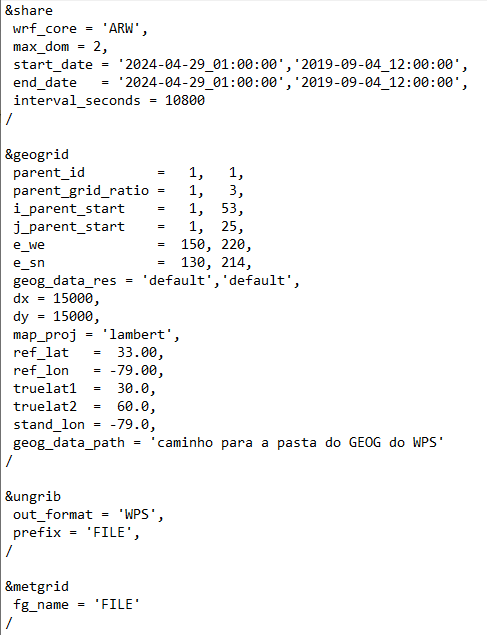
\includegraphics[width=\linewidth,height=0.78\textheight,keepaspectratio]{figuras/17db7e5e6b9358abd3cb5f6bf27aa508a9e0212b.png}
\caption{\textcolor{red}{Inserir legenda da figura.}}
\label{fig:figura-26}
\end{figure}

Dessa forma, o arquivo intermediário com prefixo FILE, contendo a condição inicial atmosférica, foi gerado a partir do arquivo GRIB-2 do GFS, conforme o fluxo exemplificado na \textcolor{red}{Figura Y}. Posteriormente, esse arquivo foi utilizado como entrada direta para a etapa subsequente de geração das condições iniciais do MPAS.

\begin{figure}[H]
\centering
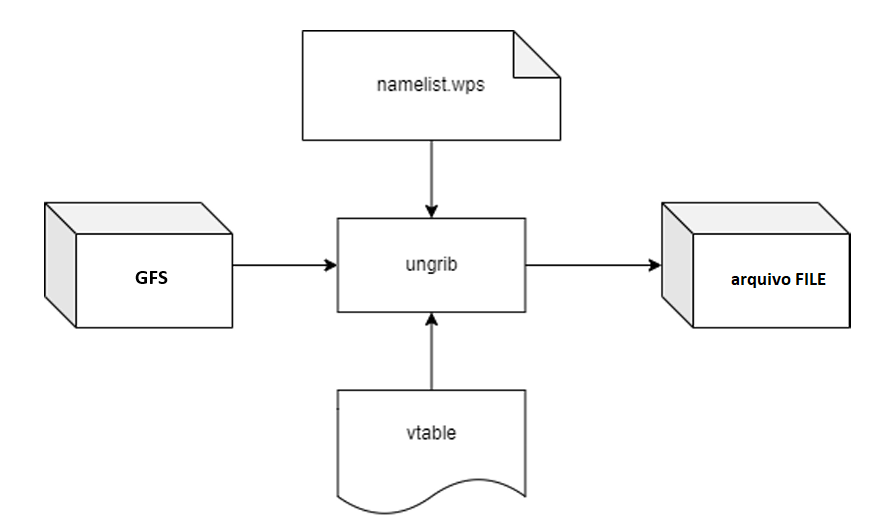
\includegraphics[width=\linewidth,height=0.78\textheight,keepaspectratio]{figuras/6ec0da5b6065816b7a59b7a20e9b02bd110fab85.png}
\caption{\textcolor{red}{Inserir legenda da figura.}}
\label{fig:figura-27}
\end{figure}

\subsubsection{Integração das condições iniciais (estáticas e dinâmicas) com a grade do MPAS}

A criação do arquivo de condições iniciais do MPAS (arquivo init) corresponde à etapa em que o estado atmosférico inicial, representado pelo arquivo FILE, e as informações estáticas do domínio (topografia, características de superfície, entre outras), previamente interpoladas para a malha escolhida e armazenadas no arquivo static, são integradas em um único arquivo init, que contém todas as informações externas necessárias para a execução da simulação com o MPAS.

Para essa integração, utiliza-se novamente o pré-processador init\_atmosphere, que, diferentemente da etapa de geração do arquivo static, passa a desempenhar um papel análogo ao do metgrid no sistema WRF, combinando os campos atmosféricos iniciais com os dados geográficos do domínio.

Nessa etapa, os arquivos de configuração utilizados são, novamente, o namelist.init\_atmosphere e o streams.init\_atmosphere. O fluxo de processamento recebe como entradas o arquivo static, previamente gerado pelo próprio init\_atmosphere em uma etapa anterior com configurações distintas, e o arquivo FILE, produzido pelo ungrib. O fluxo correspondente a essa etapa é apresentado na \textcolor{red}{Figura X}.

\begin{figure}[H]
\centering
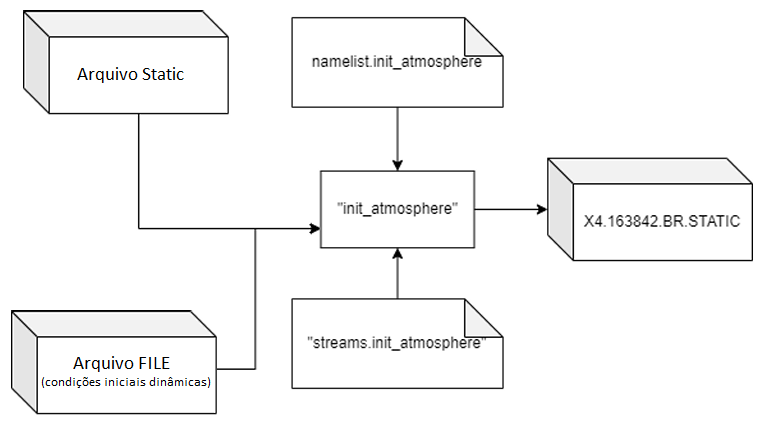
\includegraphics[width=\linewidth,height=0.78\textheight,keepaspectratio]{figuras/f73f4a7c9e0f2160b9ddb94d1c33d9bd5948c51b.png}
\caption{\textcolor{red}{Inserir legenda da figura.}}
\label{fig:figura-28}
\end{figure}

As configurações para o arquivo namelist.init\_atmosphere desta etapa estão dispostas na \textcolor{red}{tabela X}. Onde:

\begin{itemize}
\item
  config\_start\_time: Data de início da condição inicial no formato YYYY-MM-DD\_HH:MN:SS
\item
  config\_stop\_time: tabém é a data de início da condição inicial no formato YYYY-MM-DD\_HH:MN:SS caso não sejam utilizadas perturbações nas condições iniciais
\item
  config\_geog\_data\_path: é o caminho para a pasta GEOG do WPS
\item
  config\_met\_prefix: é o prefixo do arquivo contendo as informações dinâmicas de condição inicial (ou seja, o prefixo do arquivo que foi criado com o ungrib a partir das condições iniciais do GFS)
\item
  config\_block\_decomp\_file\_prefix: é o prefixo do arquivo ``part.info.part'' de particionamento da malha utilizada, que será alterado pelo MPAS de acordo com o número de processos MPI escolhidos ao rodar o modelo (como já mostrado no tópico 4.3.3.1, caso a malha não venha com o arquivo ``.info.part'' para a quantidade de processos desejada, esse deve ser criado com o MPI)
\end{itemize}

\begin{longtable}[]{@{}
  >{\raggedright\arraybackslash}p{(\columnwidth - 0\tabcolsep) * \real{1.0000}}@{}}
\caption{Configurações do arquivo \textit{namelist.init\_atmosphere} utilizadas na geração das condições iniciais do MPAS.}\label{tab:tabela-01}\\
\toprule\noalign{}
\endfirsthead
\endhead
\bottomrule\noalign{}
\endlastfoot
\texttt{\&nhyd\_model} \\
\texttt{\hspace*{1em}config\_init\_case = 7} \\
\texttt{\hspace*{1em}config\_start\_time = '2024-04-28\_01:00:00'} \\
\texttt{\hspace*{1em}config\_stop\_time = '2024-04-28\_01:00:00'} \\
\texttt{\hspace*{1em}config\_theta\_adv\_order = 3} \\
\texttt{\hspace*{1em}config\_coef\_3rd\_order = 0.25} \\
\texttt{\hspace*{1em}config\_interface\_projection = 'linear\_interpolation'} \\
\texttt{/} \\
\texttt{\&dimensions} \\
\texttt{\hspace*{1em}config\_nvertlevels = 55} \\
\texttt{\hspace*{1em}config\_nsoillevels = 4} \\
\texttt{\hspace*{1em}config\_nfglevels = 38} \\
\texttt{\hspace*{1em}config\_nfgsoillevels = 4} \\
\texttt{/} \\
\texttt{\&data\_sources} \\
\texttt{\hspace*{1em}config\_geog\_data\_path = '/home/lammoc/MPAS/MPAS-A/WPS/geog'} \\
\texttt{\hspace*{1em}config\_met\_prefix = 'FILE'} \\
\texttt{\hspace*{1em}config\_sfc\_prefix = 'SST'} \\
\texttt{\hspace*{1em}config\_fg\_interval = 86400} \\
\texttt{\hspace*{1em}config\_landuse\_data = 'MODIFIED\_IGBP\_MODIS\_NOAH'} \\
\texttt{\hspace*{1em}config\_topo\_data = 'GMTED2010'} \\
\texttt{\hspace*{1em}config\_vegfrac\_data = 'MODIS'} \\
\texttt{\hspace*{1em}config\_albedo\_data = 'MODIS'} \\
\texttt{\hspace*{1em}config\_maxsnowalbedo\_data = 'MODIS'} \\
\texttt{\hspace*{1em}config\_supersample\_factor = 3} \\
\texttt{\hspace*{1em}config\_use\_spechumd = false} \\
\texttt{/} \\
\texttt{\&vertical\_grid} \\
\texttt{\hspace*{1em}config\_ztop = 30000.0} \\
\texttt{\hspace*{1em}config\_nsmterrain = 1} \\
\texttt{\hspace*{1em}config\_smooth\_surfaces = true} \\
\texttt{\hspace*{1em}config\_dzmin = 0.3} \\
\texttt{\hspace*{1em}config\_nsm = 30} \\
\texttt{\hspace*{1em}config\_tc\_vertical\_grid = true} \\
\texttt{\hspace*{1em}config\_blend\_bdy\_terrain = false} \\
\texttt{/} \\
\texttt{\&interpolation\_control} \\
\texttt{\hspace*{1em}config\_extrap\_airtemp = 'lapse-rate'} \\
\texttt{/} \\
\texttt{\&preproc\_stages} \\
\texttt{\hspace*{1em}config\_static\_interp = false} \\
\texttt{\hspace*{1em}config\_native\_gwd\_static = false} \\
\texttt{\hspace*{1em}config\_vertical\_grid = true} \\
\texttt{\hspace*{1em}config\_met\_interp = true} \\
\texttt{\hspace*{1em}config\_input\_sst = false} \\
\texttt{\hspace*{1em}config\_frac\_seaice = false} \\
\texttt{/} \\
\texttt{\&io} \\
\texttt{\hspace*{1em}config\_pio\_num\_iotasks = 0} \\
\texttt{\hspace*{1em}config\_pio\_stride = 1} \\
\texttt{/} \\
\texttt{\&decomposition} \\
\texttt{\hspace*{1em}config\_block\_decomp\_file\_prefix = 'x4.163842.graph.info.part.'} \\
\end{longtable}

Já as configuraçções para o arquivo streams.init\_atmosphere desta etapa estão dispostas na \textcolor{red}{tabela X}. Onde:

\begin{itemize}
\item
  Primeiro filename\_template: caminho para o arquivo ``static'' gerado pelo init\_atmosphere
\item
  Segundo filename\_template: Caminho do arquivo ``init'' que será criado pelo init\_atmosphere.
\end{itemize}

\begin{longtable}[]{@{}
  >{\raggedright\arraybackslash}p{(\columnwidth - 0\tabcolsep) * \real{1.0000}}@{}}
\caption{Configurações do arquivo \textit{streams.init\_atmosphere} utilizadas na geração das condições iniciais do MPAS.}\label{tab:tabela-02}\\
\toprule\noalign{}
\endfirsthead
\endhead
\bottomrule\noalign{}
\endlastfoot
\texttt{\textless streams\textgreater} \\
\texttt{\textless immutable\_stream name="input"} \\
\phantom{\texttt{\textless immutable\_stream }}\texttt{type="input"} \\
\phantom{\texttt{\textless immutable\_stream }}\texttt{filename\_template="x4.163842\_RS.static.nc"} \\
\phantom{\texttt{\textless immutable\_stream }}\texttt{input\_interval="initial\_only" /\textgreater} \\[0.6em]
\texttt{\textless immutable\_stream name="output"} \\
\phantom{\texttt{\textless immutable\_stream }}\texttt{type="output"} \\
\phantom{\texttt{\textless immutable\_stream }}\texttt{filename\_template="x4.163842\_RS.init.nc"} \\
\phantom{\texttt{\textless immutable\_stream }}\texttt{packages="initial\_conds"} \\
\phantom{\texttt{\textless immutable\_stream }}\texttt{output\_interval="initial\_only" /\textgreater} \\[0.6em]
\texttt{\textless/streams\textgreater} \\
\end{longtable}

Com todas as configurações devidamente ajustadas, o init\_atmosphere foi executado, realizando a interpolação espacial dos campos atmosféricos do arquivo FILE para a grade não estruturada do MPAS e integrando essas informações aos dados estáticos do domínio (arquivo ``static'').

Ao final do processo, foi gerado o arquivo "init" correspondente à data inicial da simulação, compatível com o MPAS e utilizado diretamente como condição inicial para a integração temporal do modelo.

\subsubsection{Configurações para a execução do modelo MPAS}

Com o arquivo de condições iniciais (\emph{init}) corretamente gerado e disponível no diretório de execução do MPAS, a etapa seguinte consiste na configuração da simulação por meio dos arquivos namelist.atmosphere e streams.atmosphere, que definem, respectivamente, os parâmetros físicos e numéricos do modelo, e o controle dos fluxos de entrada e saída de dados durante a integração temporal.

O arquivo namelist.atmosphere é responsável por controlar os parâmetros fundamentais da simulação atmosférica, incluindo o passo de tempo, a duração total da integração, a representação espacial associada à malha, a decomposição paralela do domínio e a escolha das parametrizações físicas. Para os experimentos realizados, esses parâmetros foram definidos em função da data inicial e da resolução espacial de cada simulação. A Tabela X apresenta, a título de exemplo, a configuração adotada para um dos casos simulados, onde:

\begin{itemize}
\item
  \textbf{config\_start\_time:} Define a data e a hora de início da simulação, correspondendo ao instante da condição inicial atmosférica fornecida ao modelo, no formato YYYY-MM-DD\_HH:MN:SS.
\item
  \textbf{config\_dt:} Define o passo de tempo da simulação, que corresponde ao intervalo temporal entre sucessivas integrações do estado atmosférico e é expresso em segundos. Esse parâmetro deve ser definido em função da escala espacial característica da malha, associada ao comprimento típico das células de maior resolução, de modo a garantir a estabilidade numérica do modelo durante a integração. Para este estudo, foi calculado de acordo com a Equação~\ref{eq:passo-tempo-mpas}, onde o comprimento característico da malha é ditado pelo espaçamento (em km) entre seus pixels de menor resolução \textsuperscript{{[}33{]}}.
\end{itemize}

\begin{equation}
\label{eq:passo-tempo-mpas}
\Delta t = 6 \ast \left(\text{comprimento característico da malha}\right)
\end{equation}

\begin{itemize}
\item
  \textbf{config\_run\_duration:} Especifica o tempo total de integração do modelo em formato de dias, horas, minutos e segundos, a partir da condição inicial definida em config\_start\_time, e seguindo o formato \textquotesingle D\_HH:MN:SS\textquotesingle.
\item
  \textbf{config\_len\_disp:} Define o comprimento característico da célula de maior resolução presente no domínio, expresso em metros. Esse parâmetro representa a maior escala espacial resolvida explicitamente pelo MPAS e é utilizado internamente para ajustes numéricos e físicos dependentes da resolução da grade.
\item
  \textbf{config\_block\_decomp\_file\_prefix:} Define o prefixo do arquivo de particionamento da malha (graph.info.part). Esse arquivo contém as informações de decomposição do domínio entre os processos MPI, sendo obrigatório para a execução do MPAS. O sufixo associado ao número de processos é automaticamente ajustado pelo modelo no momento da execução, de acordo com o número de processos incluídos no comando mpi run (por meio do parâmetro -np).
\item
  \textbf{config\_physics\_suite:} Define o pacote de esquemas físicos a ser utilizado na simulação atmosférica. Esse pacote agrupa parametrizações responsáveis pela representação de processos físicos como microfísica, convecção, camada limite planetária, radiação e interações superfície--atmosfera, garantindo coerência interna entre os esquemas selecionados e simplificando a configuração do modelo.
\end{itemize}

É importante notar que, especificamente para a resolução de 60x3 km, utilizou-se a configuração ``convection\_permitting'' nessa variável, de forma a adequar as parametrizações físicas à presença de uma região da malha em escala convectiva. Enquanto as rodadas de 60x60 km e 60x10 km utilizam a suite ``mesoscale\_reference'', adequada para resoluções mais grosseiras. A suite ``convection\_permitting'' é recomendada para espaçamentos inferiores a 10 km, permitindo uma representação mais realista dos processos convectivos e da precipitação associada (UCAR, 2024).

\begin{longtable}[]{@{}
  >{\raggedright\arraybackslash}p{(\columnwidth - 0\tabcolsep) * \real{1.0000}}@{}}
\caption{Configurações principais do arquivo \textit{namelist.atmosphere} utilizadas na execução do MPAS.}\label{tab:tabela-03}\\
\toprule\noalign{}
\endfirsthead
\endhead
\bottomrule\noalign{}
\endlastfoot
\texttt{\&nhyd\_model} \\
\texttt{\hspace*{1em}config\_time\_integration\_order = 2} \\
\texttt{\hspace*{1em}config\_dt = 90} \\
\texttt{\hspace*{1em}config\_start\_time = '2024-04-28\_00:00:00'} \\
\texttt{\hspace*{1em}config\_run\_duration = '5\_00:00:00'} \\
\texttt{\hspace*{1em}config\_split\_dynamics\_transport = true} \\
\texttt{\hspace*{1em}config\_number\_of\_sub\_steps = 2} \\
\texttt{\hspace*{1em}config\_dynamics\_split\_steps = 3} \\
\texttt{\hspace*{1em}config\_horiz\_mixing = '2d\_smagorinsky'} \\
\texttt{\hspace*{1em}config\_visc4\_2dsmag = 0.05} \\
\texttt{\hspace*{1em}config\_scalar\_advection = true} \\
\texttt{\hspace*{1em}config\_monotonic = true} \\
\texttt{\hspace*{1em}config\_coef\_3rd\_order = 0.25} \\
\texttt{\hspace*{1em}config\_epssm = 0.1} \\
\texttt{\hspace*{1em}config\_smdiv = 0.1} \\
\texttt{\hspace*{1em}config\_len\_disp = 15000.0} \\
\texttt{/} \\
\texttt{\&damping} \\
\texttt{\hspace*{1em}config\_zd = 22000.0} \\
\texttt{\hspace*{1em}config\_xnutr = 0.2} \\
\texttt{/} \\
\texttt{\&limited\_area} \\
\texttt{\hspace*{1em}config\_apply\_lbcs = false} \\
\texttt{/} \\
\texttt{\&io} \\
\texttt{\hspace*{1em}config\_pio\_num\_iotasks = 0} \\
\texttt{\hspace*{1em}config\_pio\_stride = 1} \\
\texttt{/} \\
\texttt{\&decomposition} \\
\texttt{\hspace*{1em}config\_block\_decomp\_file\_prefix = 'x4.163842.graph.info.part.'} \\
\texttt{/} \\
\texttt{\&restart} \\
\texttt{\hspace*{1em}config\_do\_restart = false} \\
\texttt{/} \\
\texttt{\&printout} \\
\texttt{\hspace*{1em}config\_print\_global\_minmax\_vel = true} \\
\texttt{\hspace*{1em}config\_print\_detailed\_minmax\_vel = false} \\
\texttt{/} \\
\texttt{\&IAU} \\
\texttt{\hspace*{1em}config\_IAU\_option = 'off'} \\
\texttt{\hspace*{1em}config\_IAU\_window\_length\_s = 21600.} \\
\texttt{/} \\
\texttt{\&physics} \\
\texttt{\hspace*{1em}config\_sst\_update = false} \\
\texttt{\hspace*{1em}config\_sstdiurn\_update = false} \\
\texttt{\hspace*{1em}config\_deepsoiltemp\_update = false} \\
\texttt{\hspace*{1em}config\_radtlw\_interval = '00:30:00'} \\
\texttt{\hspace*{1em}config\_radtsw\_interval = '00:30:00'} \\
\texttt{\hspace*{1em}config\_bucket\_update = 'none'} \\
\texttt{\hspace*{1em}config\_physics\_suite = 'mesoscale\_reference'} \\
\texttt{/} \\
\texttt{\&soundings} \\
\texttt{\hspace*{1em}config\_sounding\_interval = 'none'} \\
\texttt{/} \\
\texttt{\&input} \\
\texttt{\hspace*{1em}config\_original\_latitude\_degrees = 0} \\
\texttt{\hspace*{1em}config\_original\_longitude\_degrees = 0} \\
\texttt{\hspace*{1em}config\_new\_latitude\_degrees = 40.4} \\
\texttt{\hspace*{1em}config\_new\_longitude\_degrees = -3.7} \\
\texttt{\hspace*{1em}config\_birdseye\_rotation\_counter\_clockwise\_degrees = 0} \\
\texttt{/} \\
\end{longtable}

O controle dos arquivos de entrada e saída de dados da simulação é realizado pelo arquivo streams.atmosphere por meio de ``streams'' que são denotadas por ``\textless\textgreater'', de acordo com o apresentado na \textcolor{red}{tabela x}, onde:

\begin{itemize}
\item
  \textbf{input (immutable\_stream}): Define o fluxo de entrada das condições iniciais atmosféricas do modelo. Esse stream lê o arquivo x4.163842\_RS.init.nc, que contém o estado atmosférico completo interpolado para a malha do MPAS, incluindo informações dinâmicas e termodinâmicas necessárias para o início da integração temporal. O atributo input\_interval="initial\_only" indica que esse arquivo é lido apenas uma vez, no instante inicial da simulação, sendo obrigatório para qualquer execução do MPAS-Atmosphere.
\item
  \textbf{output (stream)}: Responsável pela geração dos arquivos de histórico da simulação atmosférica. Esse stream produz arquivos no formato history.\$Y-\$M-\$D\_\$h.\$m.\$s.nc, que armazenam variáveis prognósticas e diagnósticas tridimensionais e bidimensionais, dependentes do tempo e da estrutura vertical do modelo. No caso apresentado, a frequência de escrita é de 6 horas (output\_interval="6:00:00"). As variáveis efetivamente incluídas nesses arquivos são definidas no arquivo auxiliar stream\_list.atmosphere.output.
\item
  \textbf{diagnostics (stream)}: Define o fluxo de saída destinado a variáveis diagnósticas específicas, geralmente bidimensionais ou integradas verticalmente. Os arquivos diag.\$Y-\$M-\$D\_\$h.\$m.\$s.nc são gerados a cada 3 horas (output\_interval="3:00:00"), conforme indicado no trecho fornecido. As variáveis escritas nesse stream são listadas separadamente no arquivo stream\_list.atmosphere.diagnostics, permitindo maior controle sobre os campos diagnósticos produzidos pelo modelo.
\end{itemize}

No caso dos experimentos realizados neste trabalho, as variáveis rainc e rainnc foram escritas no arquivo de diagnósticos do MPAS a cada 3 horas de simulação, sendo ambas armazenadas como valores acumulados desde o início da integração do modelo. A precipitação total foi, portanto, obtida a partir da soma dessas duas variáveis. De acordo com o MPAS-Atmosphere User's Guide, rainc corresponde à accumulated convective precipitation, enquanto rainnc representa a accumulated total grid-scale precipitation (UCAR, 2023).

\begin{longtable}[]{@{}
  >{\raggedright\arraybackslash}p{(\columnwidth - 0\tabcolsep) * \real{1.0000}}@{}}
\caption{Configurações principais do arquivo \textit{streams.atmosphere} utilizadas na execução do MPAS.}\label{tab:tabela-04}\\
\toprule\noalign{}
\begin{minipage}[b]{\linewidth}\raggedright
\textless streams\textgreater{}

\textless immutable\_stream name="input"

type="input"

\textbf{filename\_template="x4.163842\_RS.init.nc"}

input\_interval="initial\_only" /\textgreater{}

\textless immutable\_stream name="restart"

type="input;output"

filename\_template="restart.\$Y-\$M-\$D\_\$h.\$m.\$s.nc"

input\_interval="initial\_only"

output\_interval="1\_00:00:00" /\textgreater{}

\textless stream name="output"

type="output"

filename\_template="history.\$Y-\$M-\$D\_\$h.\$m.\$s.nc"

output\_interval="6:00:00" \textgreater{}

\textless file name="stream\_list.atmosphere.output"/\textgreater{}

\textless/stream\textgreater{}

\textless stream name="diagnostics"

type="output"

filename\_template="diag.\$Y-\$M-\$D\_\$h.\$m.\$s.nc"

output\_interval="3:00:00" \textgreater{}

\textless file name="stream\_list.atmosphere.diagnostics"/\textgreater{}

\textless/stream\textgreater{}

\textless stream name="surface"

type="input"

\textbf{filename\_template="x4.163842.sfc\_update.nc"}

filename\_interval="none"

input\_interval="none" \textgreater{}

\textless file name="stream\_list.atmosphere.surface"/\textgreater{}

\textless/stream\textgreater{}

\textless immutable\_stream name="iau"

type="input"

\textbf{filename\_template="x4.163842.AmB.\$Y-\$M-\$D\_\$h.\$m.\$s.nc"}

filename\_interval="none"

packages="iau"

input\_interval="initial\_only" /\textgreater{}

\textless immutable\_stream name="lbc\_in"

type="input"

filename\_template="lbc.\$Y-\$M-\$D\_\$h.\$m.\$s.nc"

filename\_interval="input\_interval"

packages="limited\_area"

input\_interval="3:00:00" /\textgreater{}

\textless/streams\textgreater{}
\end{minipage} \\
\midrule\noalign{}
\endhead
\bottomrule\noalign{}
\endlastfoot
\end{longtable}

Com os arquivos namelist.atmosphere e streams.atmosphere corretamente configurados, a execução do modelo MPAS é realizada por meio de um comando MPI, que inicializa o modelo utilizando o número de processos previamente definido. Para que a execução seja bem-sucedida, é necessário que o arquivo de particionamento da malha (graph.info) esteja presente e seja compatível com o número de processadores utilizados. O comando para executar, por exemplo, com 48 processadores é:

\textbf{\$} mpirun -np 16 ./atmosphere\_model

\subsubsection{Organização das simulações}

Conforme descrito no tópico 4.3.1, foram realizados dois experimentos neste trabalho, diferenciados exclusivamente pela data da condição inicial atmosférica, correspondentes aos dias 28/04/2024 e 29/04/2024. Para cada experimento, as simulações com o modelo MPAS foram conduzidas utilizando três grades com resoluções espaciais distintas, a saber: 60$\times$60 km, 60$\times$15 km e 60$\times$3 km, totalizando seis simulações numéricas.

Em função das diferentes demandas computacionais associadas a cada resolução espacial (em especial quanto ao consumo de memória RAM) as simulações foram executadas em infraestruturas de hardware distintas. As duas simulações realizadas com a grade de menor resolução espacial (60$\times$60 km), uma para cada experimento, foram executadas em um computador desktop do Laboratório de Monitoramento de Modelagem de Sistemas Climáticos (LAMMOC) da Universidade Federal Fluminense (UFF). Esse equipamento é composto por 32 GB de memória RAM e um processador Intel i7 de décima segunda geração, com 8 núcleos físicos, sendo utilizado apenas um deles na simulação. Cada uma dessas simulações apresentou um tempo total de execução de aproximadamente 23 horas.

As simulações com resolução intermediária (60$\times$15 km), também uma para cada experimento, foram executadas no supercomputador MareNostrum, pertencente ao Barcelona Supercomputing Center - Centro Nacional de Supercomputación (BSC). Para essas simulações, foram utilizados 672 processadores e 2688 GB de memória RAM. O tempo de execução observado para cada simulação nessa configuração foi de aproximadamente 12 minutos.

Por fim, as simulações de maior resolução espacial (60$\times$3 km) foram igualmente realizadas no supercomputador MareNostrum, no BSC. Nesse caso, foram empregados 2.226 processadores, com um total de 8.904 GB de memória RAM utilizados. O tempo total de execução para cada uma dessas simulações foi de aproximadamente 16 minutos.

Os experimentos realizados e suas principais características, incluindo datas de inicialização, resoluções espaciais, infraestrutura computacional utilizada e tempos de execução, encontram-se resumidos na \textcolor{red}{Tabela X}.

\begin{figure}[H]
\centering
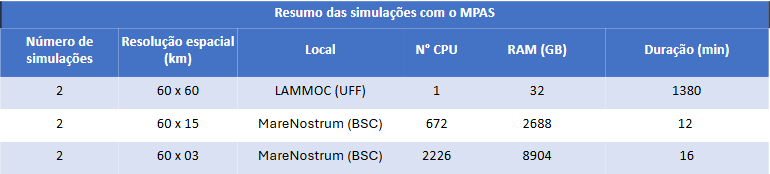
\includegraphics[width=\linewidth,height=0.78\textheight,keepaspectratio]{figuras/2f1f2cf6d4722c8084497b9992001acaf7314bc1.png}
\caption{\textcolor{red}{Inserir legenda da figura.}}
\label{fig:figura-29}
\end{figure}

\subsubsection{Pós processamento dos resultados das simulações}

Durante a execução das simulações numéricas com o MPAS, os resultados do modelo são armazenados em arquivos no formato NetCDF, organizados principalmente em dois tipos de saídas: arquivos do tipo \emph{history}, que contêm o estado prognóstico do modelo em determinados instantes de tempo, e arquivos do tipo \emph{diag}, que armazenam variáveis diagnósticas com maior frequência temporal. Para permitir a análise e visualização desses resultados em grades regulares latitude--longitude, foi utilizado o utilitário convert\_mpas, que pode ser baixado no endereço: \url{https://github.com/mgduda/convert_mpas/tree/master} .

Após compilara o programa, o processamento deve ser realizado a partir do diretório que contém os arquivos de saída do MPAS, normalmente identificados pelos padrões history*.nc e diag*.nc.

Em sua forma mais simples, o convert\_mpas pode ser aplicado diretamente a um único arquivo NetCDF do MPAS, resultando na interpolação automática das variáveis disponíveis para uma grade regular latitude--longitude. O produto dessa interpolação é armazenado em um arquivo padrão denominado latlon.nc, que ja é o produto interpolado em grade regular com todas as variáveis contidas nos arquivos diag.

Como o processo de interpolação pode ser computacionalmente custoso quando todas as variáveis são incluídas, o convert\_mpas permite restringir o conjunto de campos a serem interpolados. Para isso, pode-se criar um arquivo de texto denominado include\_fields, no qual são listados, linha a linha, os nomes das variáveis de interesse. Quando esse arquivo está presente no diretório de trabalho, apenas os campos especificados são processados, reduzindo significativamente o tempo de execução e o tamanho do arquivo de saída.

Outro aspecto importante do uso do convert\_mpas é a possibilidade de interpolar múltiplos arquivos de saída em uma única execução, consolidando diferentes instantes temporais em um único arquivo latlon.nc. Para esse tipo de operação, o primeiro argumento fornecido ao programa deve ser um arquivo NetCDF que contenha as informações da malha do MPAS (por exemplo, o arquivo static ou init), enquanto os argumentos subsequentes correspondem aos arquivos history ou diag que contêm as variáveis a serem interpoladas. O comando necessário para sua execução segue o padrão:

\$ ./convert\_mpas caminho1 caminho2

Onde, ``caminho1'' é o caminho para um arquivo com informações da malha (static ou init, por exemplo) e ``caminho2'' é o caminho para os arquivos diag resultantes da simulação.

Adicionalmente, o convert\_mpas possibilita a definição de um domínio geográfico específico para a interpolação, por meio de um arquivo denominado target\_domain. Nesse arquivo, são especificados os limites espaciais da região de interesse e o número de pontos da grade regular de saída. Essa funcionalidade é particularmente útil para análises regionais, pois reduz o volume de dados processados e concentra a interpolação em áreas específicas do domínio global do modelo.

Em todas as simulações executas, converteu-se o output dos arquivos diag apenas das variáveis rainc e rainnc e, para o caso das simulações feitas com a mais alta resolução (60x3 km) utilizou-se também da conversão somente de uma região de interesse.

Após a obtenção dos arquivos de saída interpolados em grade regular, foi desenvolvido um script em linguagem Python para a continuidade do pós-processamento. Inicialmente, reconstruiu-se a coordenada temporal real das simulações a partir da data inicial do modelo e do intervalo de saída dos diagnósticos, substituindo a dimensão temporal indexada do MPAS. Em seguida, as variáveis de precipitação acumulada RAINC e RAINNC foram desacumuladas ao longo do tempo, permitindo o cálculo da precipitação correspondente a cada intervalo de saída. As componentes convectiva e não convectiva foram então somadas para a obtenção da precipitação total por passo temporal, a qual foi armazenada em formato NetCDF. Por fim, esses dados foram agregados temporalmente para a escala diária, resultando em campos de precipitação diária total utilizados para criar as análises discutidas nos resultados e discussões.

\section{Procedimentos de avaliação das previsões}
\label{sec:procedimentos-avaliacao}

A avaliação das previsões foi realizada a partir de três abordagens complementares. Inicialmente, foi feita uma análise qualitativa dos campos diários e do acumulado total de precipitação, comparando visualmente a distribuição espacial, a intensidade e o posicionamento dos principais núcleos de chuva simulados pelos modelos em relação ao produto MERGE. Essa etapa teve como objetivo identificar os principais padrões de erro dos modelos, especialmente deslocamentos espaciais, subestimativas, superestimativas, suavização ou concentração espacial dos acumulados.

Em seguida, empregou-se o Fractions Skill Score (FSS) para quantificar a habilidade espacial dos modelos na representação das áreas de precipitação acumulada. Diferentemente de métricas ponto a ponto, como o RMSE, ou de índices categóricos de erro e acerto, o FSS é menos sensível ao problema de \textit{double penalty}, no qual estruturas de precipitação corretamente previstas em forma e intensidade, mas ligeiramente deslocadas, são penalizadas tanto pela ausência de chuva no local observado quanto pela presença de chuva em uma posição incorreta (Rossa et al., 2008). O FSS incorpora uma tolerância espacial crescente ao erro de localização, o que permite identificar a escala a partir da qual cada modelo passa a representar adequadamente a área de chuva observada, evitando que modelos de maior resolução sejam indevidamente penalizados em relação a campos mais suavizados (Mittermaier e Roberts, 2011).

O FSS, introduzido por Roberts e Lean (2008) e posteriormente implementado por Faggian (2015), pertence à classe dos métodos de verificação por vizinhança, que relaxam a exigência de correspondência exata entre previsão e observação ao avaliar a concordância espacial dentro de janelas de tamanho crescente. O cálculo é iniciado com a binarização dos campos previsto e observado, atribuindo-se valor unitário aos pontos de grade cujo acumulado iguala ou excede um limiar de precipitação previamente definido, e valor nulo aos demais. Em seguida, para cada ponto de grade, calcula-se a fração de pontos acima do limiar dentro de uma vizinhança quadrada de tamanho especificado, tanto para a previsão quanto para a observação. Dessa forma, os campos binários são convertidos em campos de frações, que representam a cobertura local do evento em cada escala espacial (Roberts e Lean, 2008).

A partir desses campos de frações, o FSS é calculado como:

\[
FSS = 1 - \frac{MSE}{MSE_{ref}}
\]

Onde \(MSE\) corresponde ao erro quadrático médio entre as frações previstas e observadas, e \(MSE_{ref}\) representa o erro quadrático médio de referência, associado ao pior caso possível de não sobreposição entre as áreas previstas e observadas acima do limiar. Essa normalização confina a métrica ao intervalo entre 0, indicativo de ausência de habilidade espacial, e 1, correspondente à concordância perfeita. Por convenção, adota-se frequentemente o valor de \(FSS \geq 0{,}5\) como critério de habilidade útil (Skok e Roberts, 2016).

Neste trabalho, o FSS foi calculado para o acumulado total do evento sobre o domínio retangular do Rio Grande do Sul, considerando diferentes limiares de precipitação acumulada e diferentes escalas espaciais de vizinhança. Como o método exige que a grade dos campos analisados seja a mesma, todos os modelos foram reamostrados para a grade do MERGE por meio de interpolação bilinear antes da aplicação da métrica.

Por fim, também foi realizada uma avaliação dos acumulados médios por bacia hidrográfica. Para isso, os campos de precipitação acumulada do MERGE e dos modelos foram recortados pelas bacias de interesse, e a diferença entre o acumulado médio previsto e observado foi calculada para cada modelo. Essa análise teve como objetivo complementar o FSS e a avaliação visual, permitindo quantificar o erro dos modelos nas regiões hidrologicamente mais relevantes do evento.

\chapter{Resultados e Discussão}

\section{Análise bruta das previsões}

\subsection{CI:28}

Em 28 de abril de 2024, o MERGE indica precipitação concentrada principalmente na porção norte/nordeste do Rio Grande do Sul, ainda com padrão relativamente disperso e sem núcleos extensos de precipitação muito elevada. Apesar disso, já são observados acumulados localizados próximos de 75 mm no dia, enquanto a metade sul do estado apresenta baixos volumes ou ausência de chuva significativa.

Em comparação com esse padrão, apenas o ETA 8 km e o BRAMS 8 km conseguiram representar de forma satisfatória o posicionamento geral da precipitação ao norte/nordeste do estado. O ETA simulou chuva nessa região, mas com campo mais suavizado e subestimativa dos acumulados observados. O BRAMS apresentou o melhor desempenho qualitativo neste dia, representando de forma mais coerente a disposição espacial da chuva e indicando o início da organização de núcleos mais intensos no setor norte, embora também tenha subestimado a magnitude da precipitação em relação ao MERGE.

As três configurações do MPAS apresentaram desempenho inferior, tanto em termos de posicionamento quanto de intensidade. Em vez de concentrar a precipitação na porção norte/nordeste, os experimentos deslocaram os acumulados para uma faixa mais central/leste do estado, o que resultou em baixa aderência espacial ao observado. Além disso, todas as configurações subestimaram a chuva diária de forma mais acentuada que o ETA e o BRAMS, principalmente em relação aos máximos observados.

De forma geral, para o primeiro dia do evento, o BRAMS apresentou o melhor desempenho relativo, seguido pelo ETA. As simulações do MPAS não representaram adequadamente a distribuição espacial da precipitação e apresentaram forte subestimativa dos acumulados.

\begin{figure}[H]
\centering
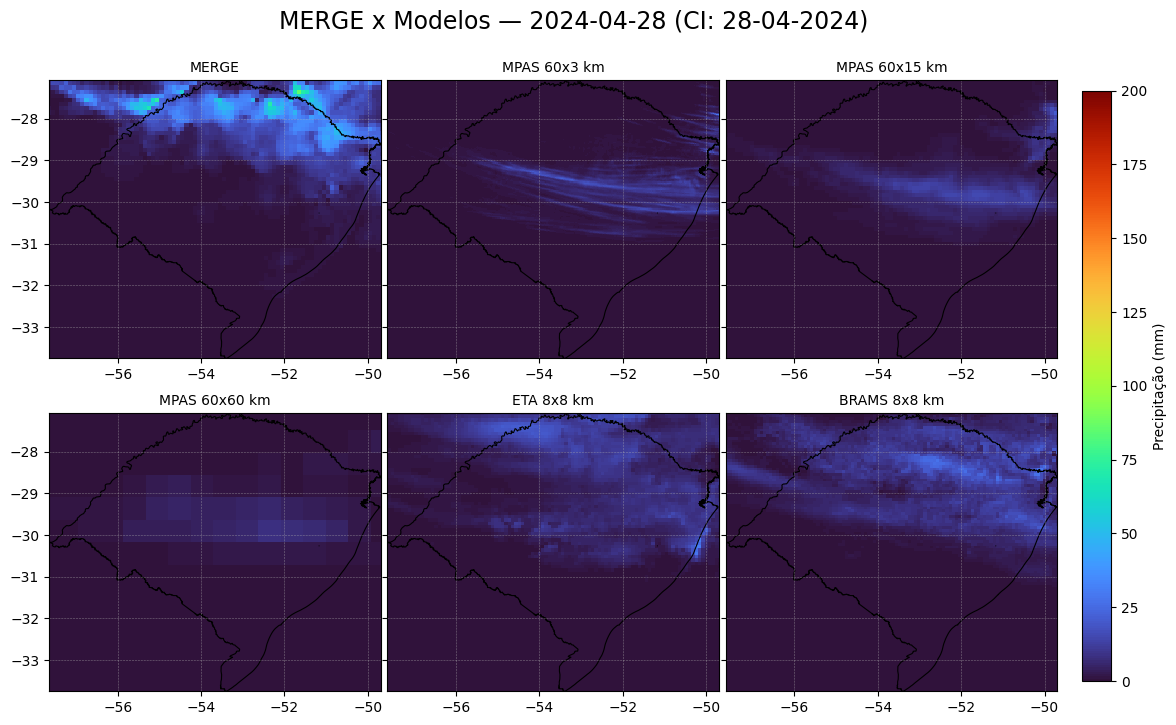
\includegraphics[width=\linewidth,height=0.78\textheight,keepaspectratio]{figuras/f9b7c4f5cfc6185c9981599ade630f36c1e49642.png}
\caption{\textcolor{red}{Inserir legenda da figura.}}
\label{fig:figura-30}
\end{figure}

Em 29 de abril de 2024, o MERGE indica intensificação e maior abrangência espacial da precipitação em relação ao dia anterior, com acumulados expressivos distribuídos por praticamente todo o Rio Grande do Sul. O campo observado apresenta uma larga faixa aproximadamente horizontal na porção central do estado, onde se organizam os núcleos mais intensos, com valores próximos de 100 mm.

Entre as configurações do MPAS, o MPAS 60$\times$3 km foi o que melhor representou a magnitude da precipitação e a organização horizontal do sistema. A simulação apresentou uma faixa de chuva intensa relativamente bem definida e com acumulados mais compatíveis com os observados no MERGE. No entanto, o principal erro esteve no posicionamento, uma vez que a banda de precipitação foi deslocada de forma significativa para o sul do estado. Sendo assim, apesar do melhor desempenho relativo em intensidade e estrutura, houve erro espacial importante.

As configurações MPAS 60$\times$15 km e MPAS 60$\times$60 km posicionaram a precipitação em latitudes menos extremas do que o MPAS 60$\times$3 km, embora ainda deslocadas para sul em relação ao observado. Por outro lado, subestimaram de forma mais acentuada os núcleos de maior precipitação, apresentando campos muito mais suavizados.

Essa diferença de comportamento não parece estar associada apenas à resolução horizontal, mas também à alteração da Physics Suite entre as simulações. Na configuração 60$\times$3 km, foi utilizada a suite convection\_permitting, mais adequada para escalas convectivas, permitindo que parte da convecção seja representada explicitamente pela dinâmica do modelo. Além disso, essa suite utiliza parametrizações distintas para convecção, microfísica, camada limite e camada superficial, o que também contribui para as diferenças observadas em relação às configurações 60$\times$15 km e 60$\times$60 km (UCAR, 2024). Essa interpretação é reforçada pela análise dos campos de saída do modelo, especialmente ``accumulated convective precipitation'' e ``accumulated total grid-scale precipitation'', nos quais se observa que os maiores acumulados simulados na rodada de maior resolução foram mais fortemente influenciados pela componente convectiva.

O ETA 8 km apresentou comportamento semelhante ao das versões mais grosseiras do MPAS. O modelo representou a precipitação em posição relativamente mais próxima em termos latitudinais do que o MPAS 60$\times$3 km, mas ainda com deslocamento para sul e forte subestimativa dos núcleos mais intensos. Já o BRAMS 8 km simulou a precipitação organizada em faixas diagonais sobre o centro/norte do estado, diferindo do padrão mais horizontal observado no MERGE. Além disso, subestimou a precipitação de forma mais acentuada que os demais modelos, especialmente na porção sul do estado.

De forma geral, para 29 de abril, o MPAS 60$\times$3 km apresentou o melhor desempenho qualitativo, principalmente por representar melhor a intensidade e a organização horizontal da precipitação, ainda que com deslocamento meridional significativo da faixa de chuva. As demais configurações do MPAS e o ETA apresentaram melhor posicionamento relativo, mas com maior suavização e subestimativa dos máximos. O BRAMS, por sua vez, apresentou a pior representação da magnitude total e organizou a precipitação em uma estrutura espacial distinta da observada, embora relativamente mais bem localizada.

\begin{figure}[H]
\centering
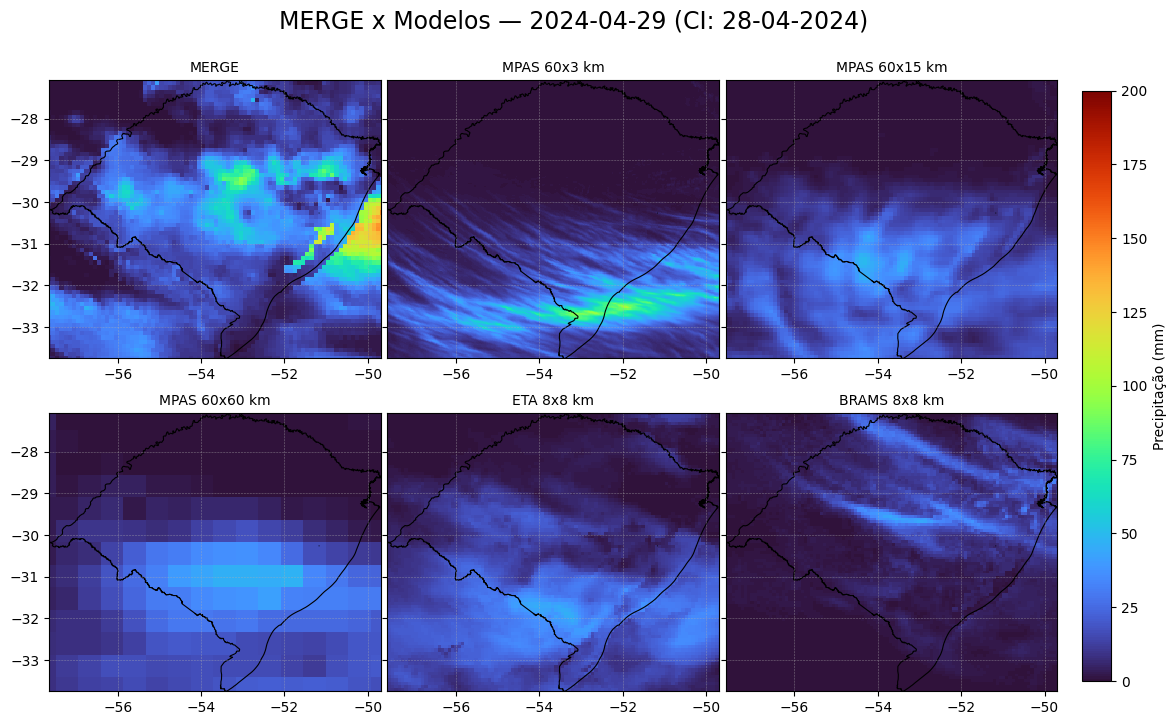
\includegraphics[width=\linewidth,height=0.78\textheight,keepaspectratio]{figuras/22d3f965472469fbb770da146e0b0411db44204e.png}
\caption{\textcolor{red}{Inserir legenda da figura.}}
\label{fig:figura-31}
\end{figure}

Em 30 de abril de 2024, o MERGE manteve um padrão espacial semelhante ao observado no dia anterior, com a precipitação organizada principalmente em uma faixa horizontal na porção central do Rio Grande do Sul. No entanto, neste dia houve intensificação expressiva dos acumulados, com formação de núcleos muito mais intensos no centro/norte do estado, atingindo valores próximos ou superiores a 200 mm no acumulado diário.

De forma geral, nenhum dos modelos conseguiu representar adequadamente a localização e a intensidade dos núcleos mais extremos observados pelo MERGE. O MPAS 60$\times$3 km foi novamente o modelo que mais se aproximou dos acumulados observados, apresentando uma faixa de precipitação mais organizada e intensa que os demais modelos embora, dessa vez, com valores bem inferiores aos observados. Além disso, a banda horizontal de chuva foi novamente deslocada de forma significativa para o sul do estado.

As configurações MPAS 60$\times$15 km e MPAS 60$\times$60 km, assim como o BRAMS 8 km, indicaram algum aumento dos acumulados diários em relação ao dia 29, mas continuaram subestimando fortemente a precipitação, principalmente os núcleos mais intensos. Essa subestimativa tornou-se ainda mais evidente neste dia, considerando a forte intensificação observada no MERGE. Além disso, esses modelos também deslocaram a principal faixa de precipitação para sul, não reproduzindo adequadamente a posição da banda observada.

O ETA 8 km apresentou o pior desempenho, mantendo acumulados muito semelhantes aos do dia anterior e, portanto, não acompanhando a intensificação da chuva observada no MERGE. Além disso, o modelo não conseguiu reproduzir a faixa horizontal organizada de precipitação representada, ainda que com limitações, pelos demais modelos, e deslocou sua precipitação excessivamente para sul em comparação com o observado.

Sendo assim, para 30 de abril, o principal erro comum aos modelos foi o deslocamento latitudinal da faixa de precipitação, com todos posicionando a banda de chuva mais ao sul do que o indicado pelo MERGE. Em termos de intensidade, o MPAS 60$\times$3 km apresentou o melhor desempenho relativo, embora ainda com erro espacial expressivo e subestimativa dos máximos. Já o ETA foi o modelo que mais subestimou a precipitação neste dia, enquanto MPAS 60$\times$15 km, MPAS 60$\times$60 km e BRAMS representaram apenas parcialmente o aumento dos acumulados, sem capturar os máximos extremos observados.

\begin{figure}[H]
\centering
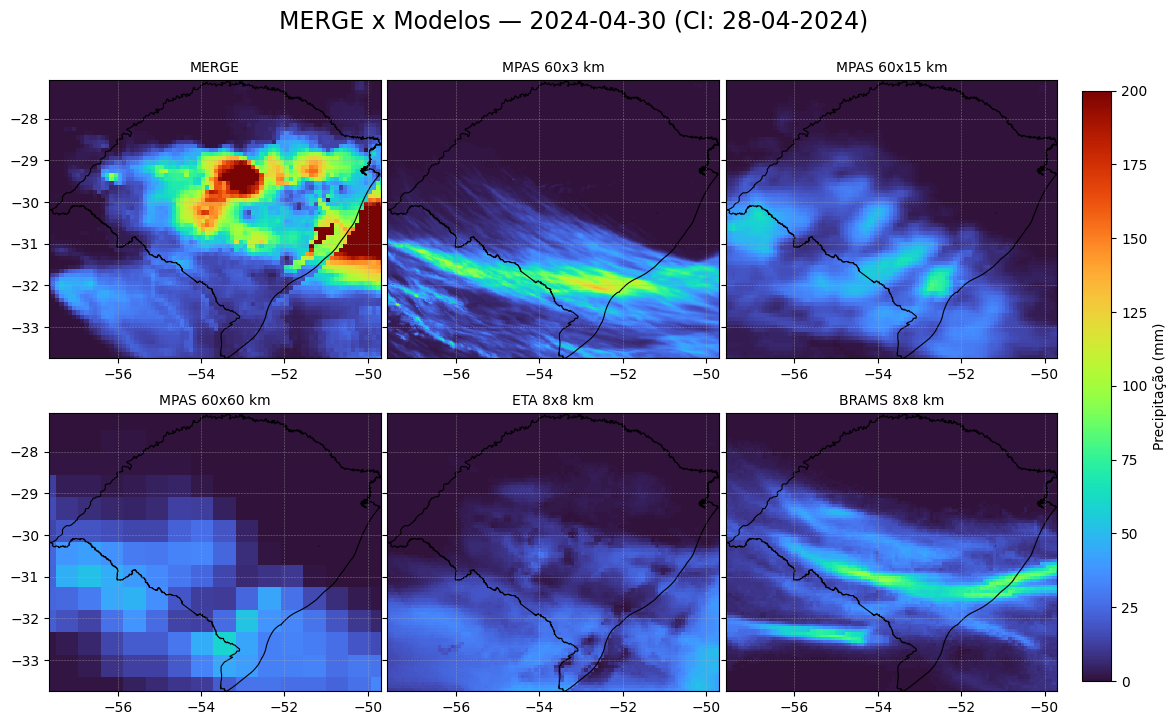
\includegraphics[width=\linewidth,height=0.78\textheight,keepaspectratio]{figuras/ac18f7aee57e4b176eaa99fe600c395b919dd664.png}
\caption{\textcolor{red}{Inserir legenda da figura.}}
\label{fig:figura-32}
\end{figure}

Em 01 de maio de 2024, o MERGE indicou precipitação ampla sobre praticamente todo o Rio Grande do Sul, com acumulados superiores a 50 mm em grande parte do estado. O padrão observado manteve a organização em faixa, mas com maior concentração dos máximos entre o Centro-Norte e o Nordeste, onde os acumulados atingiram ou ultrapassaram 200 mm no acumulado diário.

De forma geral, os modelos acompanharam parcialmente a migração latitudinal da precipitação em relação aos dias anteriores, mas todos deslocaram excessivamente a faixa principal para sudoeste. Entre as configurações do MPAS, o MPAS 60$\times$3 km novamente apresentou a estrutura e os acumulados mais próximos do observado, embora com erro espacial expressivo, posicionando os maiores volumes muito ao sul/sudoeste da área indicada pelo MERGE. O MPAS 60$\times$60 km, apesar da menor resolução e da subestimativa dos acumulados, foi o que apresentou menor erro latitudinal na posição da faixa mais intensa.

O MPAS 60$\times$15 km também representou a ocorrência de chuva significativa, mas com deslocamento para oeste/sudoeste e subestimativa dos máximos no centro-norte/nordeste do estado. O ETA 8 km apresentou o pior desempenho geral, tanto pela localização excessivamente ao sul da precipitação quanto pela forte subestimativa da intensidade, não representando adequadamente os núcleos extremos observados.

O BRAMS 8 km, por outro lado, simulou uma faixa muito intensa e concentrada, com valores localmente superiores aos observados em parte da banda. No entanto, essa precipitação ficou excessivamente estreita e deslocada para sudoeste, diferindo da distribuição mais ampla indicada pelo MERGE. Sendo assim, embora o BRAMS tenha representado acumulados elevados, sua configuração espacial apresentou baixa aderência ao campo observado.

De forma geral, o principal erro dos modelos neste dia foi o deslocamento para sudoeste da banda de precipitação intensa. O MPAS 60$\times$3 km apresentou o melhor desempenho relativo em intensidade e estrutura geral, ainda que com erro espacial importante, enquanto o ETA foi o modelo que mais subestimou a precipitação e apresentou a representação menos satisfatória do evento.

\begin{figure}[H]
\centering
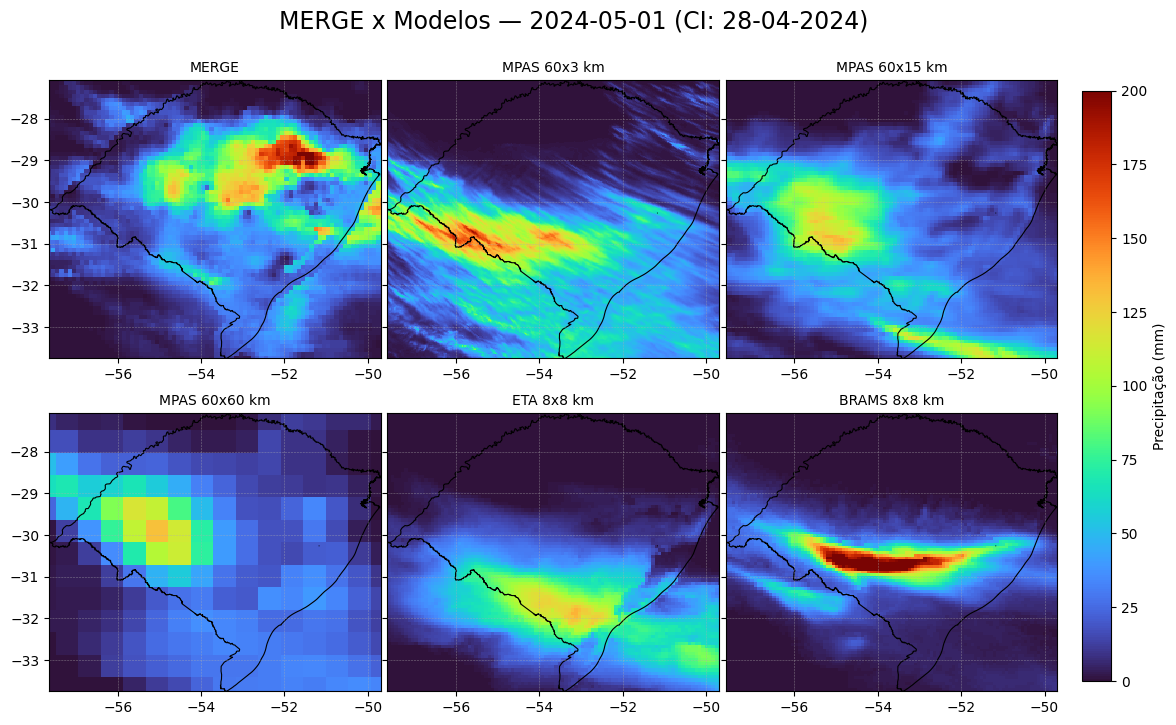
\includegraphics[width=\linewidth,height=0.78\textheight,keepaspectratio]{figuras/3376667566986f4f3dce0cf578ad584c26468f82.png}
\caption{\textcolor{red}{Inserir legenda da figura.}}
\label{fig:figura-33}
\end{figure}

Em 02 de maio de 2024, o MERGE indica a continuidade do deslocamento da precipitação para norte, iniciado entre 30 de abril e 01 de maio. A banda mais intensa passa a apresentar orientação noroeste-sudeste e concentra-se principalmente nas porções norte, centro-norte, nordeste e leste do Rio Grande do Sul, com núcleos extremos superiores a 200 mm localizados sobretudo no norte e centro-norte do estado.

Neste dia, o MPAS 60$\times$3 km apresentou o melhor desempenho qualitativo entre os modelos. Embora ainda tenha deslocado a banda de precipitação para sudoeste, conseguiu representar de forma mais satisfatória a inclinação, a estrutura espacial e a intensidade dos acumulados. Por outro lado, superestimou a área com precipitação extrema, simulando uma faixa de valores acima de 200 mm mais extensa do que a indicada pelo MERGE.

As demais configurações do MPAS também captaram melhor a distribuição geral da faixa de chuva em comparação aos dias anteriores, especialmente quanto à orientação noroeste-sudeste. No entanto, o MPAS 60$\times$15 km e o MPAS 60$\times$60 km suavizaram excessivamente o campo de precipitação e não reproduziram adequadamente os núcleos extremos. Essa diferença entre as configurações parece estar associada não apenas à maior resolução do MPAS 60$\times$3 km, mas também ao uso da suite convection\_permitting, que permite maior participação da dinâmica resolvida na representação da convecção, ao contrário das configurações com grades mais grosseiras, que utilizam a suite mesoscale\_reference.

O BRAMS 8 km representou valores máximos relativamente próximos aos observados, mas subestimou a extensão da área de precipitação extrema. Além disso, apesar de captar a inclinação da faixa de chuva, posicionou-a excessivamente ao sul e manteve a precipitação muito concentrada espacialmente. O ETA 8 km apresentou novamente o pior desempenho, com forte subestimativa dos acumulados extremos e baixa aderência à distribuição espacial observada.

De forma geral, para 02 de maio, o MPAS 60$\times$3 km foi o modelo que melhor representou a intensidade e a organização espacial da precipitação, ainda que com deslocamento para sudoeste e superestimativa da área extrema. O ETA apresentou o pior desempenho, enquanto MPAS 60$\times$15 km, MPAS 60$\times$60 km e BRAMS captaram parcialmente a estrutura da banda, mas com limitações importantes em termos de intensidade, extensão e posicionamento dos máximos.

\begin{figure}[H]
\centering
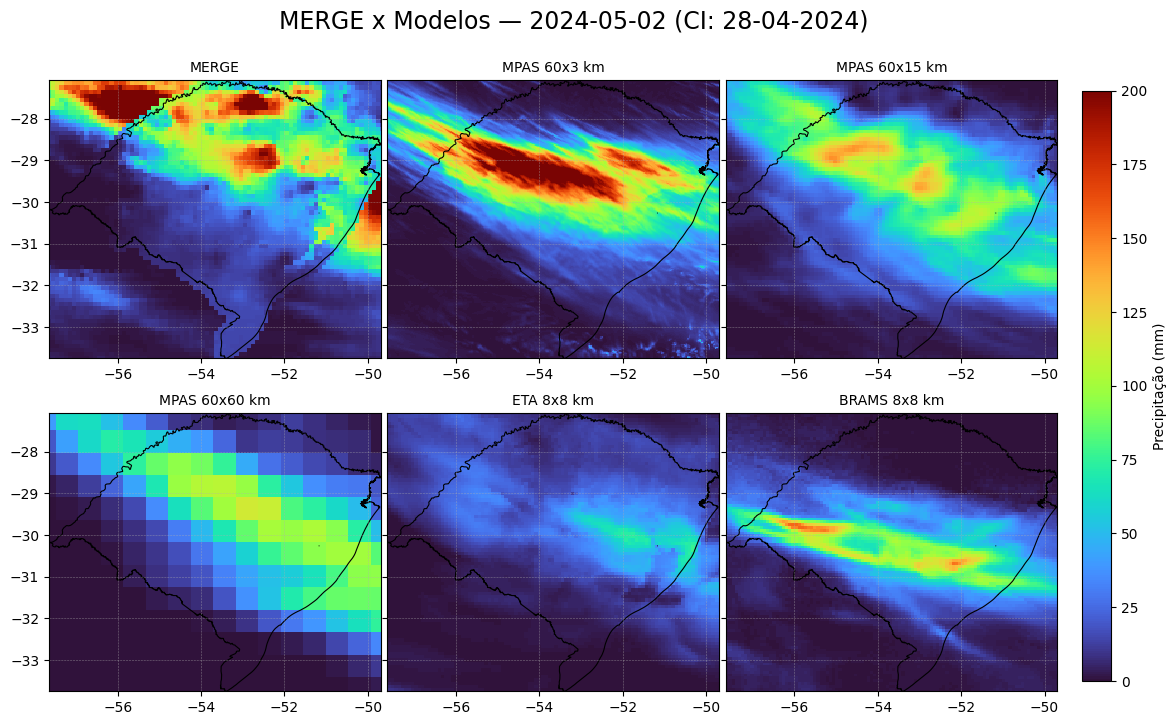
\includegraphics[width=\linewidth,height=0.78\textheight,keepaspectratio]{figuras/fc79dc2a54fef1cf42ec2eff43eead94660d1e14.png}
\caption{\textcolor{red}{Inserir legenda da figura.}}
\label{fig:figura-34}
\end{figure}

No acumulado entre 28 de abril e 02 de maio de 2024, o MERGE apresentou precipitação muito elevada sobre grande parte do centro-norte e nordeste do Rio Grande do Sul, com acumulados superiores a 300 mm e alguns focos adicionais no norte e leste do estado. Esses valores são coerentes com a validação apresentada na Seção 4.2, tanto em relação ao observado nas estações quanto aos impactos registrados durante o evento (apresentados na seção 1.3), o que sugere boa aderência do campo do MERGE ao comportamento geral da precipitação no período.

Em comparação com esse padrão, nenhum dos modelos conseguiu representar adequadamente a distribuição espacial da área com acumulados superiores a 300 mm, sendo que a maior parte deles sequer atingiu essa magnitude. Apenas o BRAMS 8 km e o MPAS 60x3 km apresentaram acumulados dessa ordem. O BRAMS foi o que simulou a maior área com precipitação extrema, mas a deslocou excessivamente para sudoeste, além de subestimar justamente os acumulados nas regiões mais afetadas. Nesse sentido, embora tenha representado melhor a magnitude máxima, apresentou erro espacial mais pronunciado.

O MPAS 60x3 km apresentou o melhor desempenho qualitativo geral. Ainda que tenha subestimado a extensão da área com acumulados superiores a 300 mm, conseguiu representar de forma mais coerente a localização das faixas de precipitação mais intensa, mesmo que com valores mais próximos de 200 mm em parte dessas áreas. Além disso, representou relativamente bem a dispersão dos acumulados superiores a 100 mm pelo estado, embora com superestimativa na porção sul e subestimativa ao norte.

Já as configurações MPAS 60x15 km e MPAS 60x60 km também conseguiram representar essa dispersão mais ampla dos acumulados, mas subestimaram de forma mais acentuada os núcleos extremos e deslocaram mais intensamente a distribuição geral para sudoeste, o que resultou em subestimativa no norte e nordeste e superestimativa relativa no sul.

O ETA 8 km apresentou o pior desempenho entre os modelos, com subestimativa notável da precipitação acumulada e posicionamento excessivamente ao sul, em parte quase fora do estado. De forma geral, os resultados indicam que o MPAS 60x3 km foi o modelo mais consistente na representação do evento, principalmente por apresentar melhor desempenho relativo em termos de localização e estrutura espacial da precipitação mais intensa, ainda que com limitações importantes na magnitude dos máximos acumulados.

\begin{figure}[H]
\centering
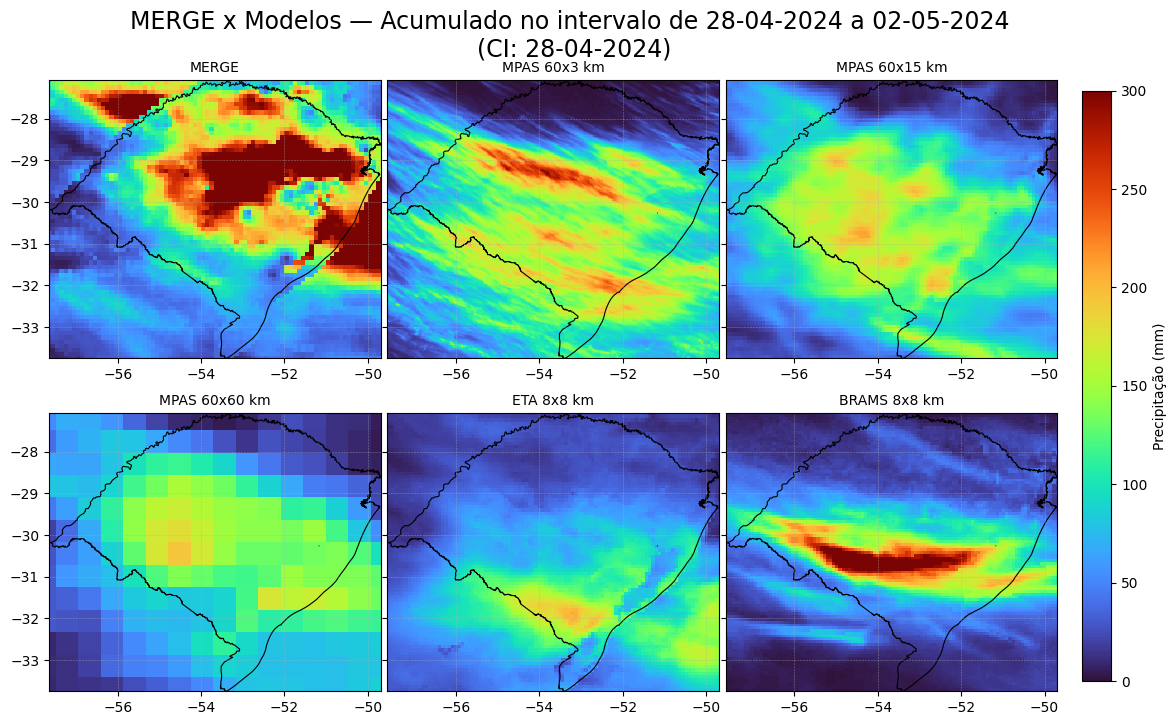
\includegraphics[width=\linewidth,height=0.78\textheight,keepaspectratio]{figuras/f35c70cb0501193885a8e6c2cb601b9d951248c0.png}
\caption{\textcolor{red}{Inserir legenda da figura.}}
\label{fig:figura-35}
\end{figure}

De forma geral, a simulação com condição inicial em 28 de abril apresentou limitações importantes na representação da evolução espacial e temporal da precipitação durante o evento. O MERGE indicou intensificação progressiva da chuva entre 28 de abril e 02 de maio, com deslocamento dos maiores acumulados para o centro-norte, norte e nordeste do Rio Grande do Sul, resultando em áreas superiores a 300 mm no acumulado total do evento.

Em comparação com esse padrão, nenhum dos modelos conseguiu representar adequadamente, ao mesmo tempo, a localização, a intensidade e a extensão dos maiores acumulados. O erro mais recorrente foi o deslocamento da precipitação para sul ou sudoeste, principalmente nos dias de maior intensidade, o que resultou em subestimativa nas regiões mais afetadas ao norte/nordeste e, em alguns casos, superestimativa relativa na porção sul do estado.

Entre os modelos avaliados, o MPAS 60$\times$3 km apresentou o melhor desempenho qualitativo geral, sobretudo por representar melhor a estrutura e a localização relativa das faixas mais intensas de precipitação. Ainda assim, manteve erro espacial importante e subestimou a extensão da área com acumulados extremos no total do evento. As configurações MPAS 60$\times$15 km e MPAS 60$\times$60 km apresentaram campos mais suavizados e maior subestimativa dos máximos, enquanto o BRAMS simulou acumulados extremos, mas com precipitação excessivamente concentrada e deslocada. O ETA 8 km apresentou o pior desempenho geral, principalmente pela forte subestimativa e pelo posicionamento excessivamente ao sul da área de chuva.

\subsection{CI:29}

Em 29 de abril de 2024, o MERGE apresentou precipitação bem distribuída pelo Rio Grande do Sul, com acumulados próximos ou superiores a 50 mm em grande parte do estado. O campo observado indica uma faixa aproximadamente horizontal na porção central, onde se organizaram os núcleos de maior intensidade, com valores próximos de 100 mm, enquanto o restante do estado manteve precipitação mais espalhada e, em geral, menos intensa.

Em comparação com esse padrão, o MPAS 60$\times$3 km apresentou forte subestimativa sobre grande parte do estado, principalmente no centro-norte e leste, onde praticamente não representou os acumulados observados. A simulação concentrou a principal faixa de precipitação muito ao sul do posicionamento indicado pelo MERGE, com uma banda mais larga e intensa do que a observada na região de maior precipitação do MERGE (central), mas seguindo a mesma orientação horizontal dos acumulados. Sendo assim, o erro parece estar mais associado ao posicionamento do sistema precipitante do que à incapacidade de gerar acumulados elevados. Em relação à simulação com CI em 28 de abril, observa-se posicionamento semelhante da faixa principal, mas com maior intensificação e concentração dos acumulados.

O MPAS 60$\times$15 km representou melhor a presença de precipitação no centro e leste do estado quando comparado às demais configurações do MPAS. Embora a faixa principal ainda tenha sido deslocada para sudoeste, a simulação manteve valores e formato dos núcleos mais intensos mais próximos do observado, especialmente em comparação com a rodada iniciada em 28 de abril.

O MPAS 60$\times$60 km e o ETA 8 km apresentaram dificuldade em representar os maiores acumulados. O MPAS 60$\times$60 km também subestimou a precipitação mais espalhada acima de 25 mm no centro e norte do estado, enquanto o ETA representou relativamente melhor essa distribuição de menores acumulados, mas falhou na intensificação dos núcleos principais. Em ambos os casos, o comportamento foi bastante semelhante ao observado na simulação com CI em 28 de abril.

O BRAMS 8 km alterou de forma mais evidente seu comportamento em relação à condição inicial anterior, simulando uma faixa intensa orientada no eixo noroeste-sudeste, posicionada ao sul da região central do estado. Embora tenha representado uma banda de precipitação mais intensa, com acumulados próximos ou superiores a 100 mm, o modelo não reproduziu a orientação preferencial mais horizontal observada no MERGE. Além disso, assim como o MPAS 60$\times$3 km, superestimou localmente os maiores valores e manteve a chuva excessivamente concentrada espacialmente.

De forma geral, para 29 de abril, o MPAS 60$\times$15 km apresentou o melhor desempenho qualitativo relativo, principalmente por representar de maneira mais adequada os valores e parte da estrutura dos núcleos mais intensos, ainda que com deslocamento espacial importante para sudoeste. O MPAS 60$\times$3 km indicou melhor capacidade de gerar acumulados elevados, mas posicionou a faixa principal de forma muito ao sul e concentrada, deixando de captar chuva em praticamente todo o estado. O BRAMS também simulou valores intensos, porém com orientação e concentração pouco aderentes ao observado, enquanto ETA e MPAS 60$\times$60 km apresentaram maior dificuldade na representação dos máximos acumulados.

\begin{figure}[H]
\centering
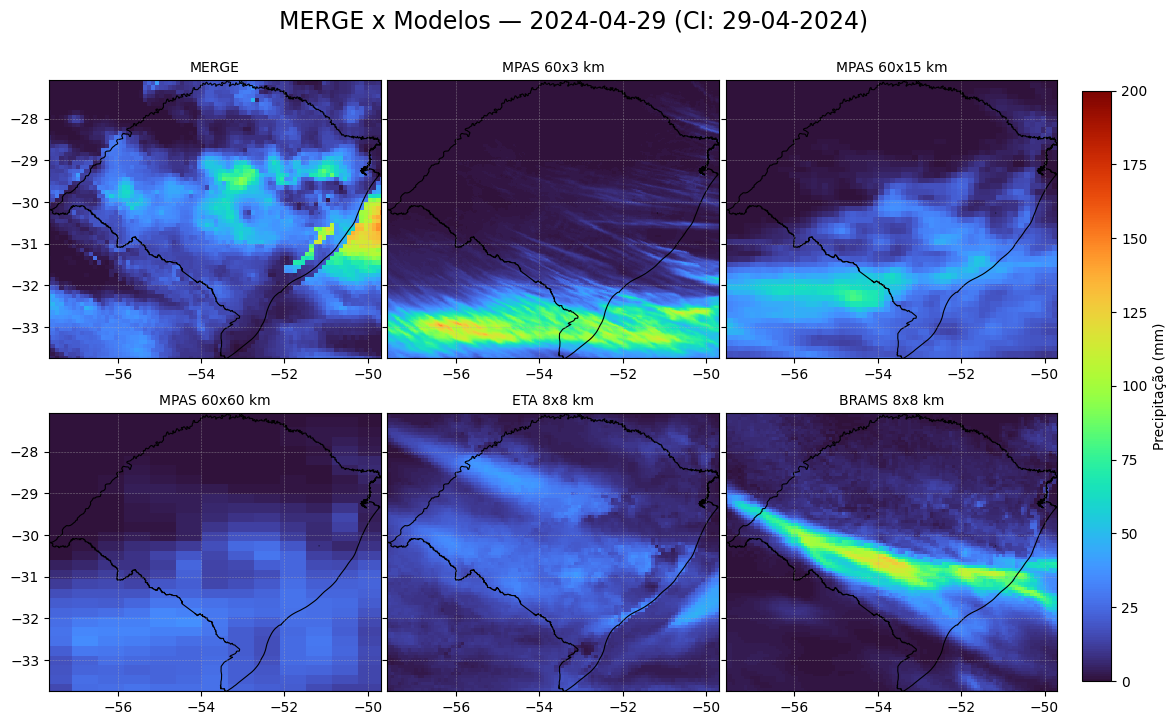
\includegraphics[width=\linewidth,height=0.78\textheight,keepaspectratio]{figuras/5c05e6500f8caf8b892c0255bec160fcbcc66569.png}
\caption{\textcolor{red}{Inserir legenda da figura.}}
\label{fig:figura-36}
\end{figure}

Em 30 de abril de 2024, o MERGE manteve uma distribuição espacial semelhante à observada no dia anterior, com precipitação organizada em uma faixa aproximadamente horizontal na porção central do Rio Grande do Sul. No entanto, nesse dia houve intensificação considerável dos acumulados, com núcleos muito mais intensos e valores superiores a 200 mm no acumulado diário, especialmente ao longo da região central do estado.

Em comparação com esse padrão, nenhum dos modelos conseguiu representar de forma satisfatória, ao mesmo tempo, a localização e a intensidade dos núcleos mais intensos. Além disso, quando comparadas às simulações com condição inicial em 28 de abril, as previsões com CI em 29 de abril apresentaram desempenho consideravelmente inferior para esse dia, principalmente em relação à representação dos máximos acumulados. Todos os modelos subestimaram fortemente a precipitação extrema, sendo que apenas o MPAS 60$\times$3 km e o BRAMS 8 km indicaram alguns pontos com acumulados próximos de 100 mm, enquanto o MERGE apresentava múltiplos núcleos acima de 150--200 mm.

Em termos de localização e distribuição espacial, o BRAMS 8 km apresentou o melhor desempenho qualitativo relativo, pois conseguiu posicionar seus acumulados mais intensos, entre aproximadamente 75 e 100 mm, em latitudes mais próximas daquelas onde o MERGE indicou os maiores acumulados em terra. Apesar disso, o padrão espacial ainda foi pouco preservado, principalmente porque os núcleos extremos não foram representados e a precipitação simulada permaneceu muito menos intensa do que a observada.

O MPAS 60$\times$3 km também conseguiu simular alguns acumulados mais elevados, mas não representou adequadamente a magnitude dos máximos e manteve erro relevante na organização espacial da precipitação. Os demais modelos apresentaram limitações ainda mais acentuadas, tanto em intensidade quanto em posicionamento, com forte subestimativa dos núcleos extremos e baixa aderência à distribuição espacial observada no MERGE.

De forma geral, para 30 de abril, o principal erro das simulações com CI em 29 de abril foi a forte subestimativa da precipitação extrema, acompanhada de erros importantes na localização da banda de chuva. O BRAMS 8 km apresentou o melhor desempenho relativo em termos de posicionamento dos maiores acumulados, ainda que com intensidade muito inferior à observada. O MPAS 60$\times$3 km foi um dos poucos modelos a indicar valores próximos de 100 mm, mas, assim como os demais, não conseguiu representar adequadamente os núcleos mais intensos do evento.

\begin{figure}[H]
\centering
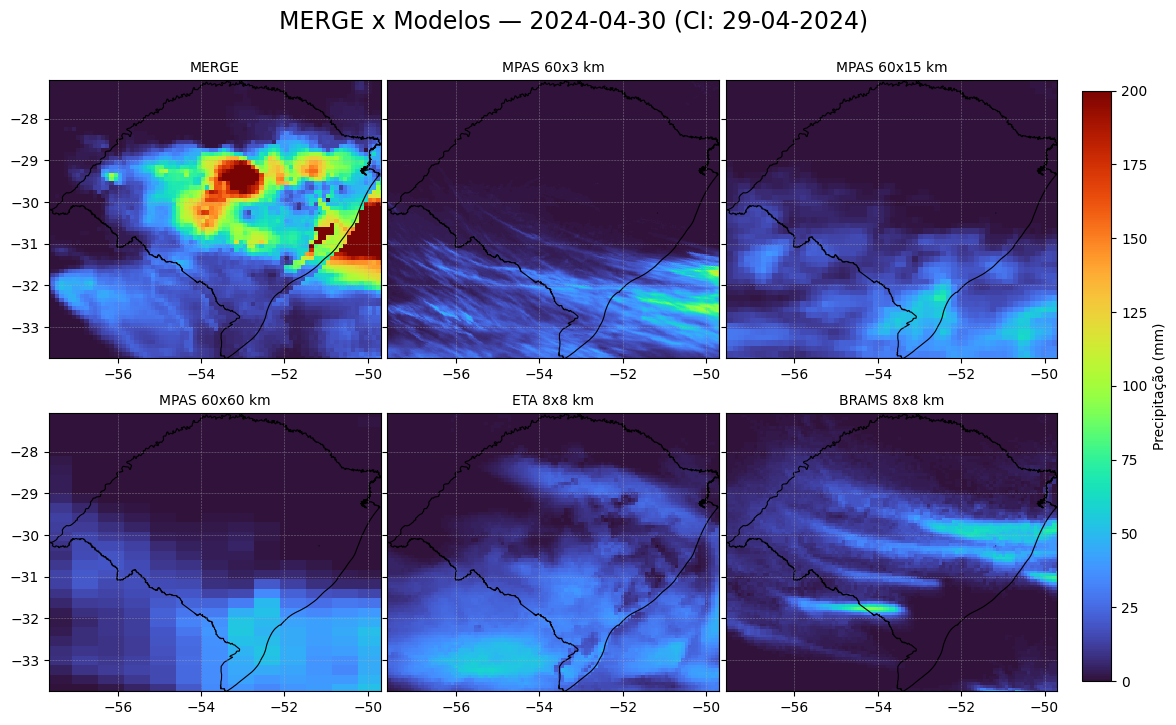
\includegraphics[width=\linewidth,height=0.78\textheight,keepaspectratio]{figuras/bbbe35dec7e45050551af35c8f727861e7af4f80.png}
\caption{\textcolor{red}{Inserir legenda da figura.}}
\label{fig:figura-37}
\end{figure}

Em 01 de maio de 2024, o MERGE apresentou chuva de ao menos 50 mm em praticamente todo o Rio Grande do Sul, com os maiores acumulados concentrados principalmente entre o centro-norte e o nordeste do estado. Nessa região, observa-se novamente a presença de núcleos extremos, com valores superiores a 200 mm no acumulado diário, indicando a manutenção de um padrão de precipitação ampla, mas com intensificação mais localizada nos setores mais ao norte do estado.

Em comparação com esse padrão, os modelos acompanharam parcialmente a migração latitudinal da faixa de precipitação em relação aos dias anteriores, com exceção do BRAMS, que já apresentava seus máximos posicionados em latitudes mais centrais. No entanto, todos deslocaram a precipitação excessivamente para sudoeste. Quando comparadas às simulações com CI em 28 de abril, as rodadas com CI em 29 de abril apresentaram, de forma geral, faixas de precipitação mais concentradas, com valores menores e pior representação da distribuição espacial indicada pelo MERGE.

Diferentemente do observado na simulação com CI em 28 de abril, o BRAMS 8 km apresentou o melhor desempenho qualitativo neste dia. A simulação representou melhor a posição relativa da faixa de precipitação intensa e apresentou melhora em relação à sua contraparte com CI anterior. Apesar disso, o modelo ainda concentrou excessivamente a chuva, embora menos do que antes, e manteve deslocamento para sudoeste da banda principal, o que limitou sua aderência ao campo observado.

Os demais modelos (MPAS 60x3 km, MPAS 60x60 km, MPAS 60x15 km e ETA 8 km) apresentaram desempenho inferior em termos de representação dos núcleos mais intensos e da distribuição espacial da precipitação, principalmente quando comparados às suas respectivas simulações com CI em 28 de abril. De forma geral, tiveram comportamento relativamente semelhante entre si, com subestimativa dos maiores acumulados e deslocamento espacial importante em relação ao MERGE.

Sendo assim, para 01 de maio, o BRAMS 8 km foi o modelo com melhor desempenho relativo, principalmente por representar de forma menos inadequada o posicionamento da faixa de maior precipitação. Ainda assim, nenhum dos modelos reproduziu adequadamente a intensidade e a distribuição espacial dos núcleos extremos observados, e a simulação com CI em 29 de abril apresentou desempenho geral inferior ao obtido com a condição inicial do dia 28.

\begin{figure}[H]
\centering
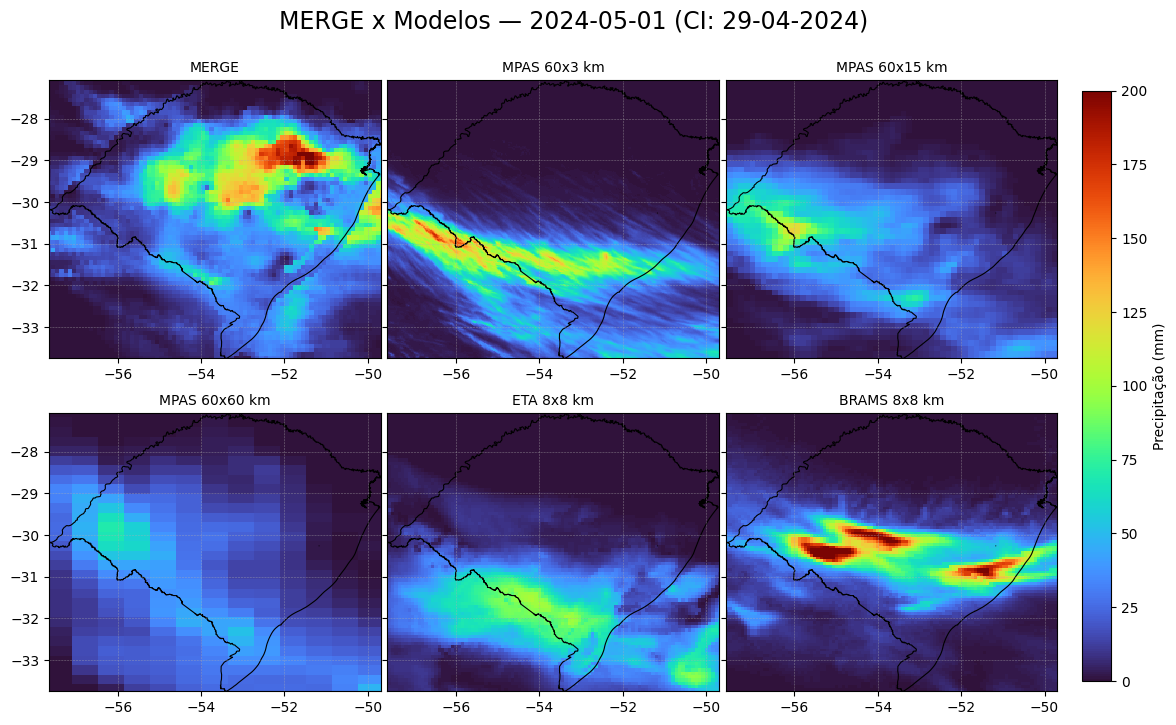
\includegraphics[width=\linewidth,height=0.78\textheight,keepaspectratio]{figuras/47fcf379f19d1daa757950cdc8177cac696f9055.png}
\caption{\textcolor{red}{Inserir legenda da figura.}}
\label{fig:figura-38}
\end{figure}

Em 02 de maio de 2024, o MERGE indica a continuidade do deslocamento da precipitação para norte, iniciado entre 30 de abril e 01 de maio. A banda mais intensa passa a apresentar orientação noroeste-sudeste e concentra-se principalmente nas porções norte, centro-norte, nordeste e leste do Rio Grande do Sul, com núcleos extremos superiores a 200 mm localizados sobretudo no norte e centro-norte do estado.

Em comparação com esse padrão, observa-se que, em relação às suas respectivas simulações com CI em 28 de abril, quase todos os modelos deslocaram a faixa de precipitação mais ao sul, com exceção do BRAMS. Além disso, com exceção do MPAS 60$\times$15 km e do ETA 8 km, os modelos apresentaram, de forma geral, núcleos menos intensos do que em suas contrapartes com condição inicial anterior. Sendo assim, apesar de alguns modelos ainda captarem parcialmente a organização da banda de chuva, a representação da intensidade e do posicionamento dos maiores acumulados foi, em geral, mais limitada.

O MPAS 60$\times$3 km apresentou novamente o melhor desempenho qualitativo entre os modelos para este dia, principalmente por representar de forma mais adequada a estrutura geral e a intensidade relativa da precipitação. No entanto, sua vantagem em relação ao MPAS 60$\times$15 km diminuiu consideravelmente, sobretudo porque, na simulação com CI em 29 de abril, o MPAS 60$\times$3 km apresentou núcleos menos intensos do que sua contraparte com CI em 28 de abril. O MPAS 60$\times$15 km, nesse sentido, manteve desempenho relativamente próximo, ainda que também com limitações na localização e na intensidade dos máximos.

O ETA 8 km manteve comportamento bastante semelhante ao observado na simulação com CI em 28 de abril, mas com aumento da área de precipitação próxima de 100 mm. Apesar disso, o modelo continuou distante de representar adequadamente a distribuição espacial indicada pelo MERGE. O MPAS 60$\times$60 km, por outro lado, manteve acumulados máximos de intensidade semelhante, mas reduziu consideravelmente a faixa de precipitação máxima, o que diminuiu sua capacidade de representar a abrangência do evento em comparação com a CI anterior.

O BRAMS 8 km apresentou algumas faixas menores com acumulados entre aproximadamente 100 e 125 mm mais ao norte do que em sua versão com CI em 28 de abril, o que permitiu representar valores mais intensos em regiões onde os demais modelos praticamente não captaram o sinal do MERGE. No entanto, o modelo também espalhou mais sua faixa de precipitação intensa, tornando os maiores acumulados mais dispersos e menos compatíveis com a estrutura espacial observada. De forma geral, para 02 de maio, o MPAS 60$\times$3 km manteve o melhor desempenho relativo, embora com menor vantagem em relação ao MPAS 60$\times$15 km, enquanto os demais modelos apresentaram limitações importantes na representação conjunta da intensidade, localização e organização espacial da banda de precipitação.

\begin{figure}[H]
\centering
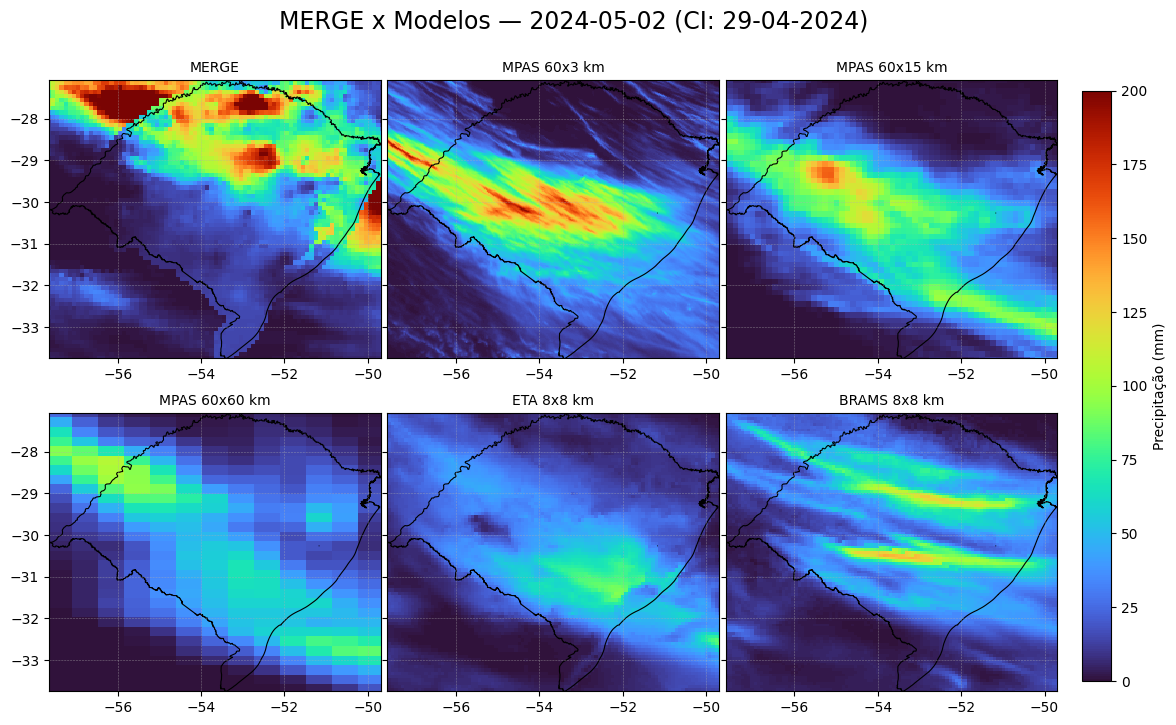
\includegraphics[width=\linewidth,height=0.78\textheight,keepaspectratio]{figuras/7bbb11ba544605c13b63010ab30a05fb25d6a3a4.png}
\caption{\textcolor{red}{Inserir legenda da figura.}}
\label{fig:figura-39}
\end{figure}

Em 03 de maio de 2024, o MERGE indica forte redução da precipitação sobre grande parte do Rio Grande do Sul, com acumulados muito baixos e chuva residual mais restrita ao setor norte/nordeste do domínio. Esse padrão sugere o enfraquecimento e o deslocamento do sistema precipitante principal em relação aos dias anteriores.

Em comparação com o observado, os modelos ainda mantiveram precipitação residual mais intensa e espalhada sobre o norte do estado, indicando atraso na representação do deslocamento e enfraquecimento do sistema. Esse erro foi mais evidente nas configurações do MPAS, que superestimaram a precipitação de forma mais acentuada que o ETA 8 km e o BRAMS 8 km.

O ETA 8 km manteve chuva fraca a moderada em áreas relativamente extensas, principalmente no centro-leste e norte. Já o BRAMS 8 km restringiu melhor a chuva à porção norte/nordeste e, embora ainda tenha superestimado localmente os acumulados residuais, foi o modelo que mais se aproximou do padrão observado.

De forma geral, para 03 de maio, o principal erro das simulações foi a persistência excessiva da precipitação, especialmente nas versões do MPAS. O BRAMS apresentou o melhor desempenho qualitativo relativo, principalmente por representar de forma mais coerente a redução e a localização da chuva residual.

\begin{figure}[H]
\centering
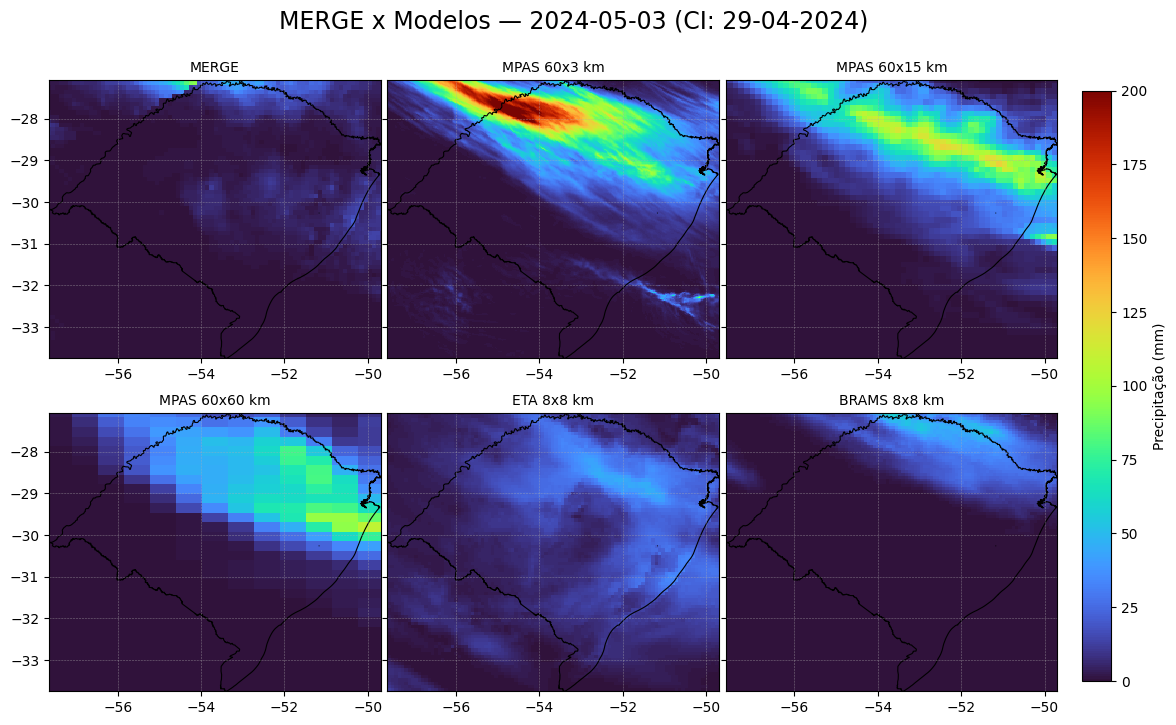
\includegraphics[width=\linewidth,height=0.78\textheight,keepaspectratio]{figuras/41cc23ad160ae2a6e40044e6f20f97124ed7811f.png}
\caption{\textcolor{red}{Inserir legenda da figura.}}
\label{fig:figura-40}
\end{figure}

No acumulado total do evento, o MERGE apresentou precipitação muito elevada em grande parte do centro-norte e nordeste do Rio Grande do Sul, com áreas superiores a 300 mm e alguns focos adicionais no norte e leste do estado. Como discutido na Seção 4.2, esses acumulados são coerentes com o observado nas estações durante o evento e também com os impactos registrados nas regiões mais afetadas, especialmente na região hidrográfica do Guaíba, já apresentada na Seção 1.3.

Em comparação com esse padrão, nenhum dos modelos conseguiu representar adequadamente a distribuição espacial da área com acumulados superiores a 300 mm, sendo que a maior parte deles sequer atingiu essa magnitude. Quando comparada à simulação com condição inicial em 28 de abril, a mudança mais evidente no acumulado total ocorreu principalmente no MPAS 60$\times$3 km, no MPAS 60$\times$60 km e no BRAMS 8 km. No caso do MPAS 60$\times$3 km, houve redução dos acumulados máximos e subestimativa mais acentuada justamente nas áreas mais afetadas, o que, em conjunto com as análises diárias, indica piora no desempenho geral do modelo em relação à CI anterior.

Comportamento semelhante é observado no MPAS 60$\times$60 km, que reduziu os acumulados em praticamente toda a sua faixa principal de precipitação quando comparado à simulação com CI em 28 de abril. Sendo assim, embora ainda represente parte da distribuição geral da chuva, o modelo passa a subestimar com mais intensidade os maiores acumulados, indicando também queda no desempenho geral do evento.

O BRAMS 8 km apresentou comportamento oposto. A simulação passou a estimar uma área maior de precipitação intensa, mais próxima do padrão indicado pelo MERGE, além de distribuir os acumulados menores de maneira mais coerente pelo restante do estado. Esse comportamento, somado às análises individuais dos dias anteriores, sugere que o BRAMS foi o único modelo com melhora relativa na simulação com CI em 29 de abril. No entanto, seu principal erro permaneceu associado ao deslocamento da faixa principal de precipitação para sudoeste, o que fez com que o modelo ainda falhasse em representar corretamente os acumulados nas áreas mais afetadas.

De forma geral, para o acumulado total do evento na simulação com CI em 29 de abril, o BRAMS 8 km apresentou o melhor desempenho qualitativo relativo, principalmente por representar melhor a extensão da precipitação intensa e a distribuição dos acumulados menores no estado. Ainda assim, nenhum modelo reproduziu adequadamente a localização e a magnitude dos máximos observados, e o deslocamento espacial dos principais núcleos de precipitação continuou sendo a principal limitação da simulação.

\begin{figure}[H]
\centering
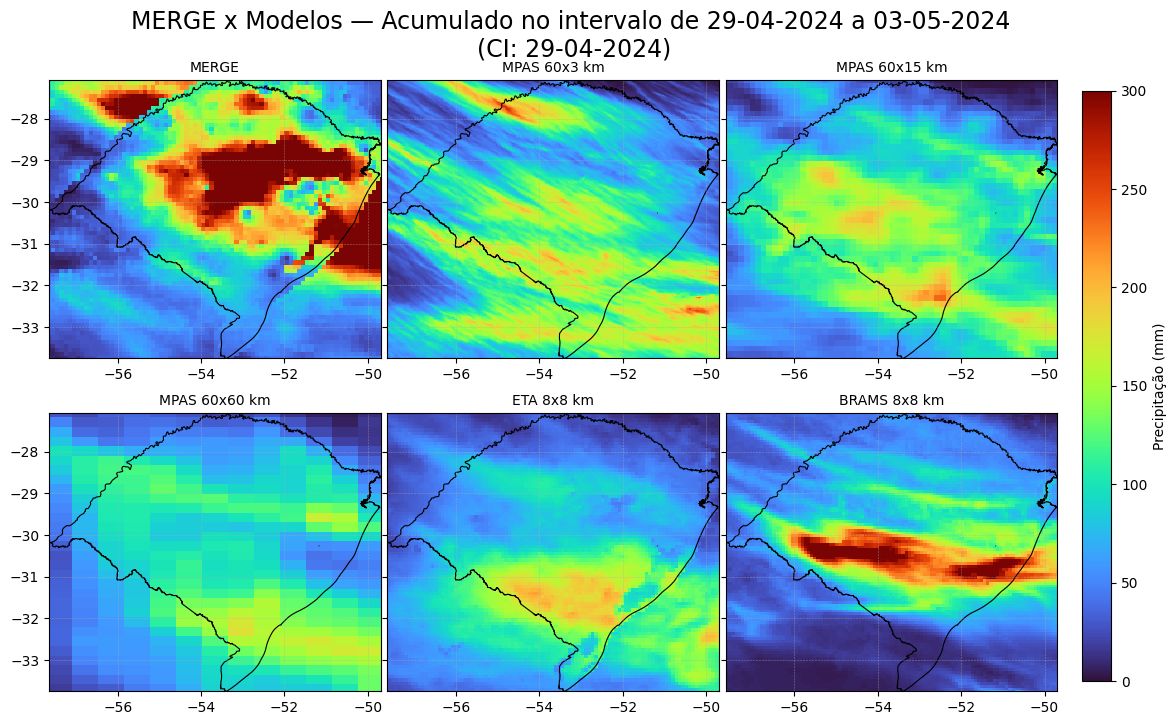
\includegraphics[width=\linewidth,height=0.78\textheight,keepaspectratio]{figuras/7fe9b5b837ea0a7445b3a158a1d7f57be42d9739.png}
\caption{\textcolor{red}{Inserir legenda da figura.}}
\label{fig:figura-41}
\end{figure}

Deste modo, a mudança da condição inicial de 28 para 29 de abril não resultou em melhora generalizada das previsões (como era de se esperar, dado a maior proximidade temporal com os maiores acumulados). Pelo contrário, a maior parte dos modelos apresentou pior representação dos máximos acumulados, com exceção do BRAMS, que melhorou em termos de abrangência e intensidade relativa, embora ainda com erro espacial importante.

Essa piora nos resultados, associada ao fato de que os maiores acumulados do evento ocorreram entre 28/04 e 02/05, indica que a simulação com condição inicial em 28 de abril apresentou melhor representação geral do evento. Sendo assim, para o restante deste trabalho, essa simulação será adotada como padrão, e todas as análises subsequentes serão realizadas a partir dela.

\subsection{Análise por Fraction Skill Score}
\label{sec:fss-resultados}

Aplicando o procedimento descrito na Seção~\ref{sec:procedimentos-avaliacao}, o FSS foi calculado para o acumulado total do evento, considerando diferentes limiares de precipitação e escalas espaciais de vizinhança. A análise a seguir apresenta os resultados obtidos para cada limiar, de forma a avaliar como a habilidade espacial dos modelos varia conforme a intensidade da precipitação acumulada e a tolerância espacial considerada.

Para o limiar de 100 mm no acumulado do evento, observa-se que todos os modelos, com exceção do ETA 8 km, apresentaram algum grau de habilidade espacial, com aumento sistemático do FSS à medida que a escala espacial da janela aumenta \textcolor{red}{(Figura 1)}. O MPAS 60$\times$60 km apresentou os maiores valores em todas as escalas, partindo de aproximadamente 0,67 em 25 km e atingindo valores próximos de 0,84 em 200 km. Esse comportamento indica boa correspondência espacial para a área mais ampla de precipitação acumulada acima de 100 mm, ainda que essa habilidade esteja associada a um campo mais suavizado. Em seguida, aparecem o MPAS 60$\times$15 km e o MPAS 60$\times$3 km, com valores bastante próximos entre si, ambos superiores a 0,5 já na menor escala analisada. O BRAMS 8 km apresentou desempenho intermediário, enquanto o ETA 8 km manteve os menores valores de FSS, permanecendo abaixo de 0,4 mesmo na escala de 200 km.

\begin{figure}[H]
\centering
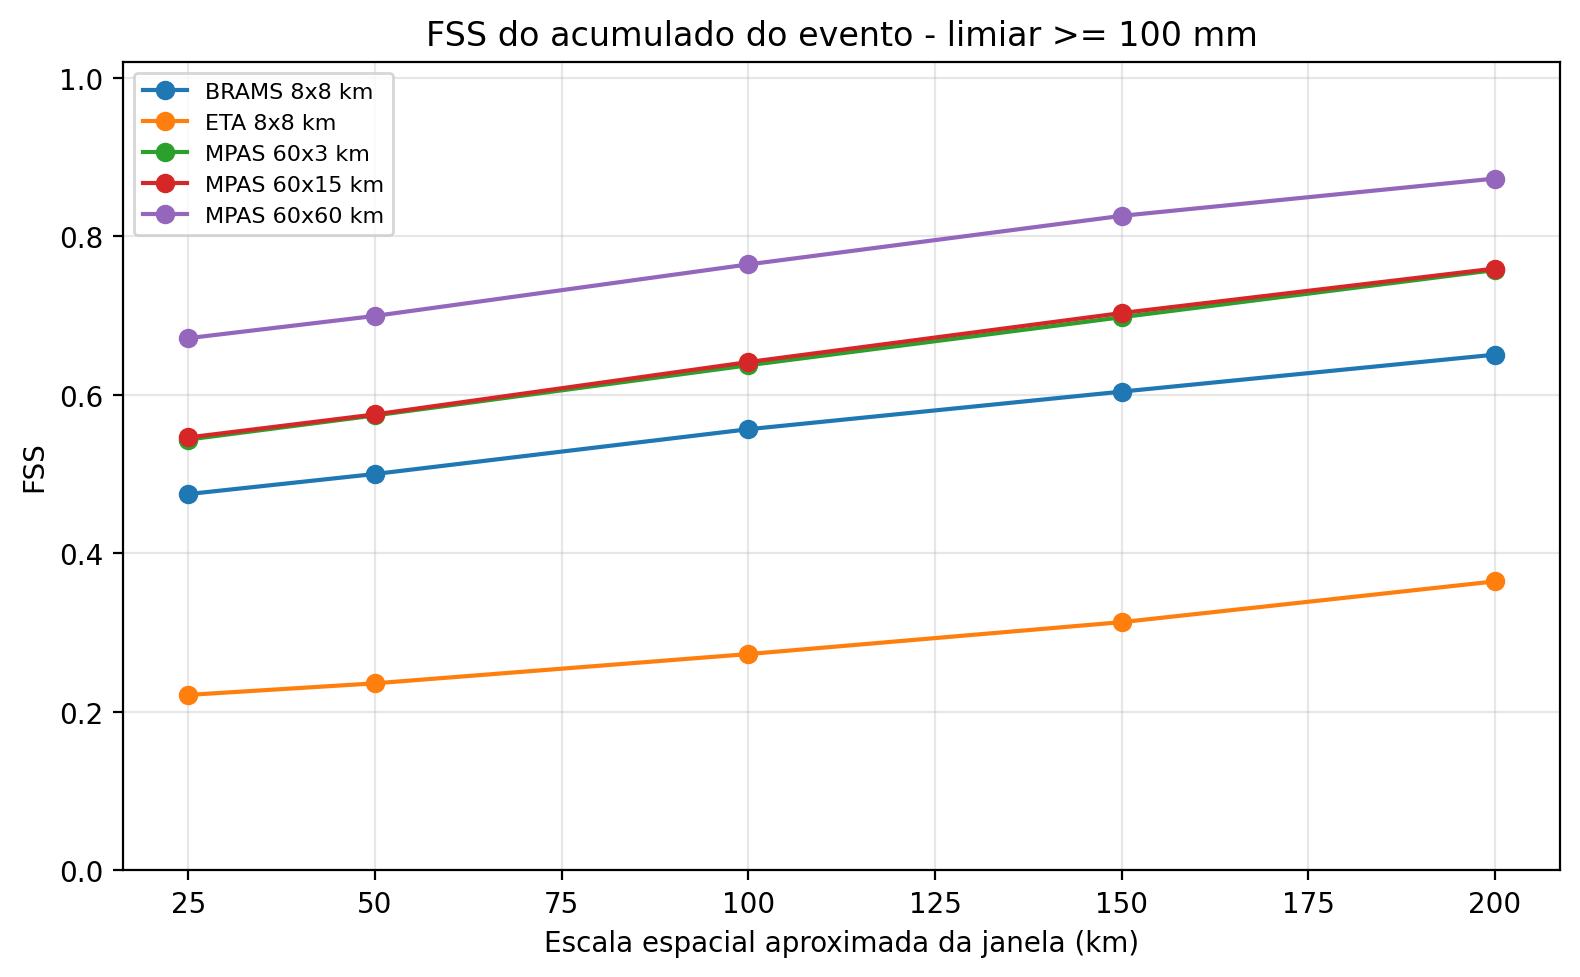
\includegraphics[width=\linewidth,height=0.78\textheight,keepaspectratio]{figuras/bdf300abe42e7e743a374e1b736c7799b2a0b1b1.png}
\caption{\textcolor{red}{Inserir legenda da figura.}}
\label{fig:figura-42}
\end{figure}

Esse resultado mostra que, para limiares mais baixos, a melhor pontuação não necessariamente corresponde ao modelo com melhor representação dos máximos acumulados. O desempenho superior do MPAS 60$\times$60 km na \textcolor{red}{Figura 1} está provavelmente associado à maior abrangência e suavização do campo de precipitação, o que favorece a sobreposição espacial com áreas extensas de chuva acumulada acima de 100 mm. Esse padrão é coerente com a análise qualitativa, na qual as configurações mais grosseiras do MPAS representaram parcialmente a distribuição geral da precipitação, embora com perda dos núcleos mais intensos. Portanto, nesse limiar, o FSS favorece a capacidade de reproduzir a extensão espacial da chuva acumulada, mais do que a representação dos extremos.

Quando o limiar é elevado para 150 mm, o desempenho dos modelos se altera de forma clara \textcolor{red}{(Figura 2}). O MPAS 60$\times$3 km passa a apresentar os maiores valores de FSS em todas as escalas, com crescimento de aproximadamente 0,36 em 25 km para cerca de 0,64 em 200 km. Além disso, é o único modelo que ultrapassa o valor de 0,5, o que ocorre apenas a partir da escala de 150 km. Esse comportamento indica que, embora o MPAS 60x3 km tenha apresentado maior capacidade de representar espacialmente áreas de precipitação intermediária em relação aos outros modelos, ainda foi necessária grande tolerância espacial. Evidenciando assim a dificuldade de previsão do evento analisado.

\begin{figure}[H]
\centering
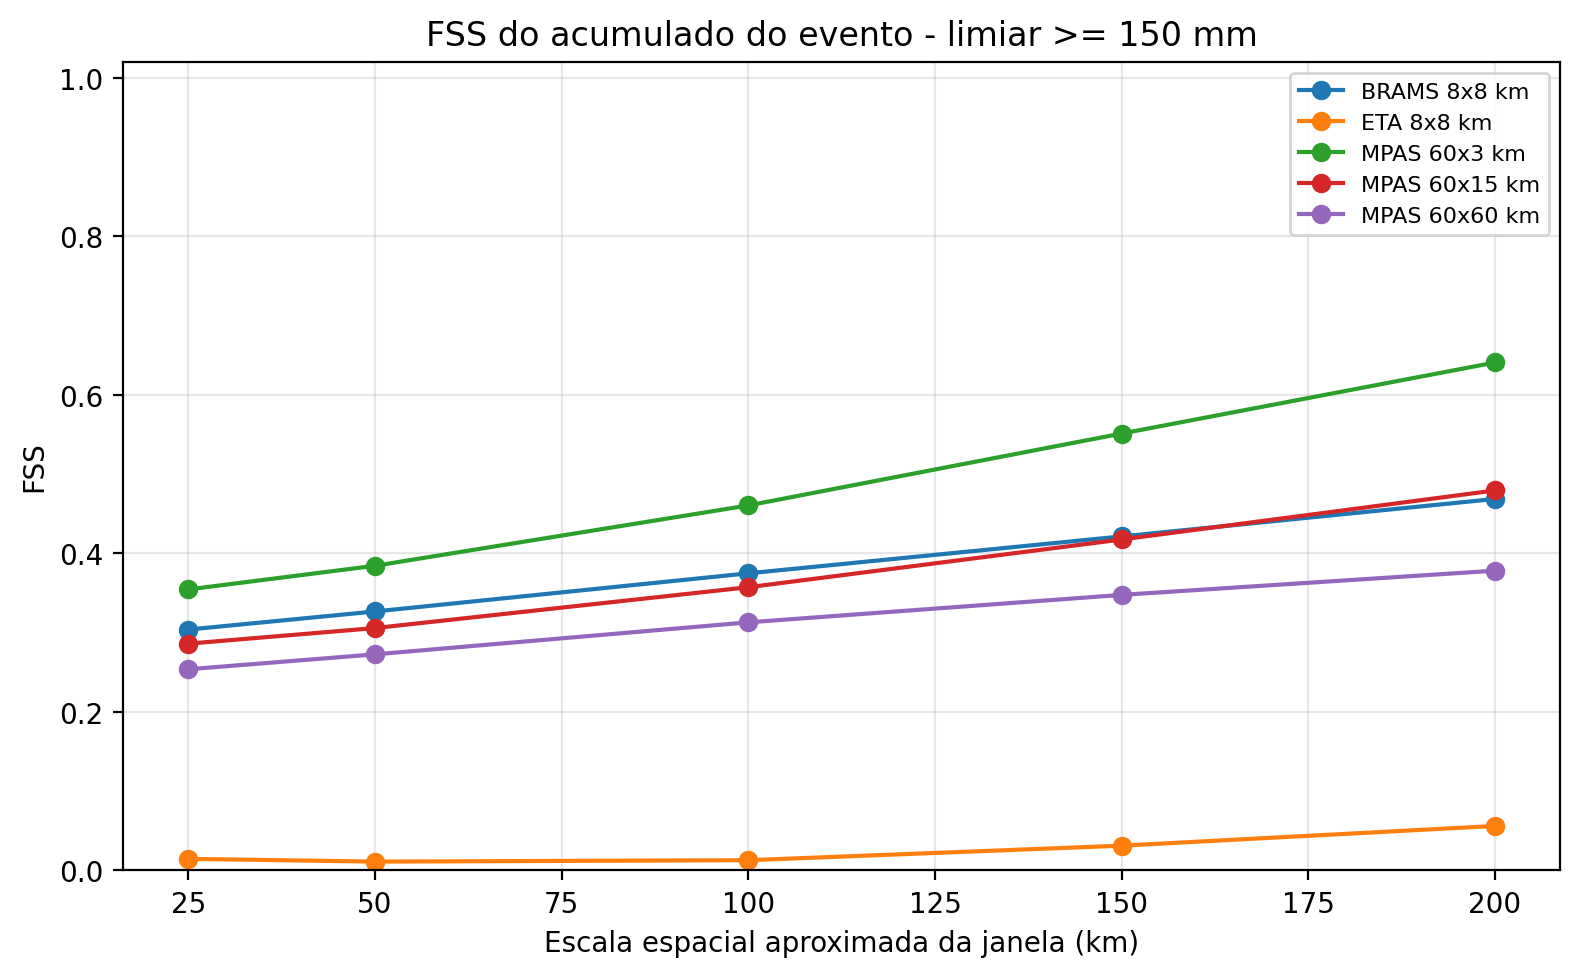
\includegraphics[width=\linewidth,height=0.78\textheight,keepaspectratio]{figuras/f25db557cb6d8f4cfad42078c11e748f72f2962a.png}
\caption{\textcolor{red}{Inserir legenda da figura.}}
\label{fig:figura-43}
\end{figure}

Ainda na \textcolor{red}{Figura 2}, o BRAMS 8 km e o MPAS 60$\times$15 km apresentaram desempenho intermediário, com valores crescentes em função da escala, mas sem atingir FSS superior a 0,5. O MPAS 60$\times$60 km, que havia apresentado o melhor desempenho para 100 mm, perde habilidade relativa quando o limiar é elevado para 150 mm, reforçando a limitação dessa configuração na representação até mesmo de acumulados intermediários. O ETA 8 km, por sua vez, apresentou valores praticamente nulos em pequenas e médias escalas, com apenas leve aumento em 200 km, confirmando a forte subestimativa já indicada pela análise qualitativa das previsões brutas.

Para o limiar de 200 mm, a separação entre os modelos e também a perda de desempenho geral tornam-se ainda mais evidentes (\textcolor{red}{Figura 3}). O MPAS 60$\times$3 km mantém os maiores valores de FSS nas escalas de 25 a 150 km, variando de aproximadamente 0,21 a 0,35. O BRAMS 8 km apresenta valores menores nas escalas iniciais, mas aumenta progressivamente com a escala e se aproxima do MPAS 60$\times$3 km em 200 km, quando ambos atingem valores próximos de 0,35. Esse comportamento sugere que o BRAMS representou parte dos acumulados elevados, mas com maior erro de posicionamento, de modo que sua habilidade só se torna comparável à do MPAS 60$\times$3 km com uma grande tolerância espacial.

\begin{figure}[H]
\centering
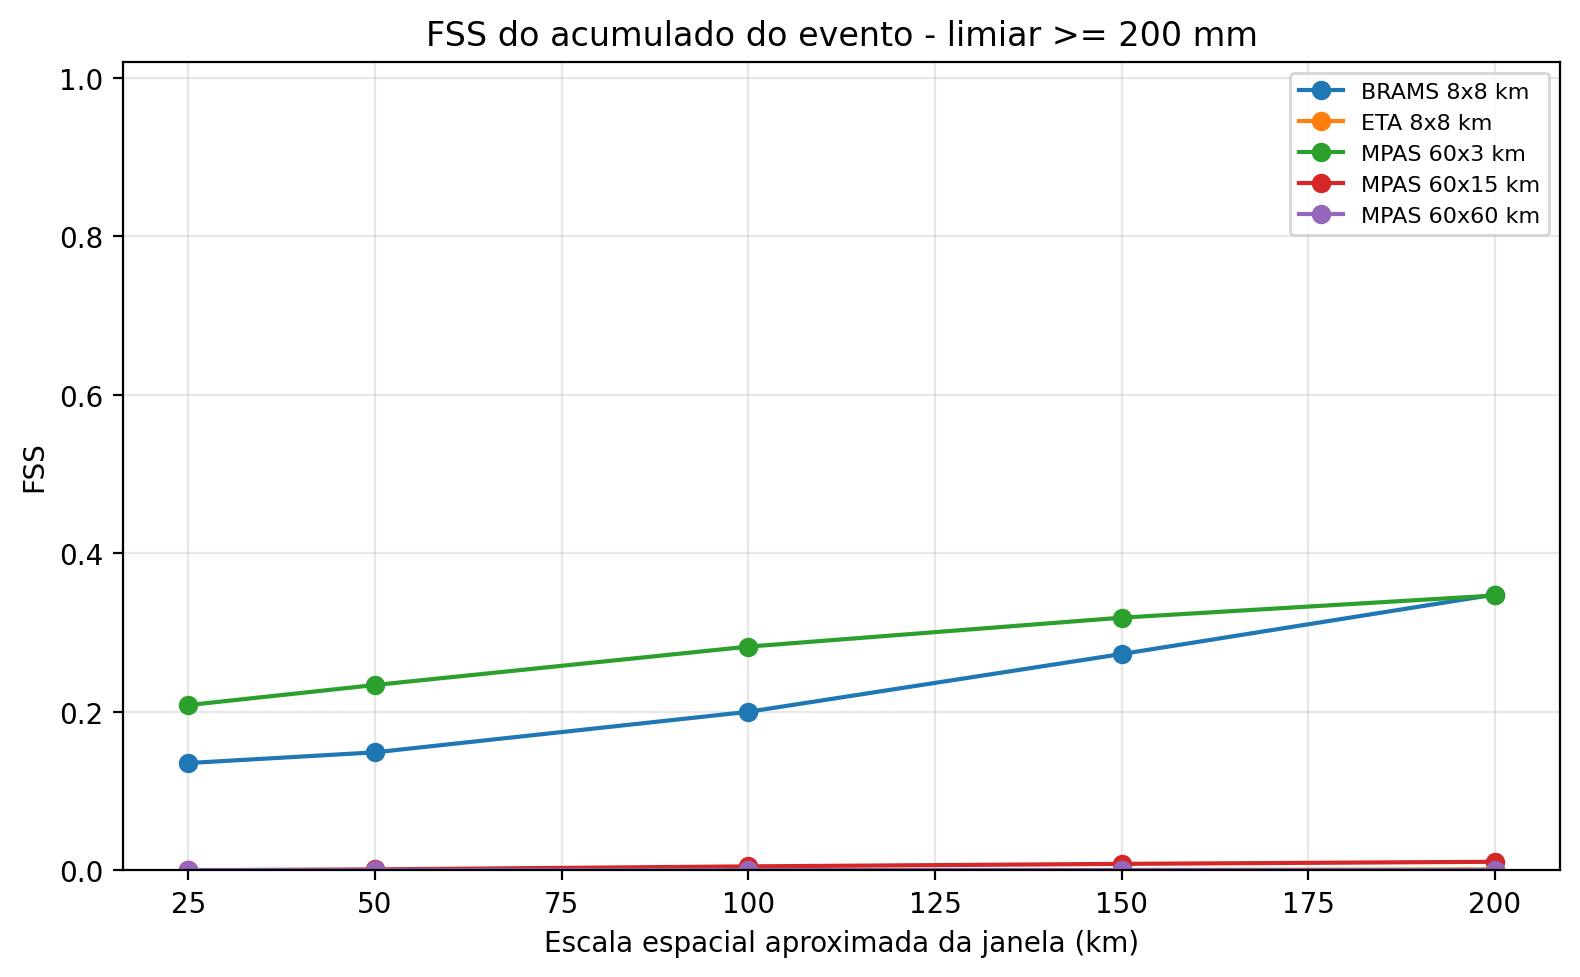
\includegraphics[width=\linewidth,height=0.78\textheight,keepaspectratio]{figuras/0cda3e2ff6592b947b0398f19f089a4f314b95c8.png}
\caption{\textcolor{red}{Inserir legenda da figura.}}
\label{fig:figura-44}
\end{figure}

Os demais modelos apresentaram FSS próximo de zero para o limiar de 200 mm. O MPAS 60$\times$15 km manteve apenas valores residuais, enquanto o MPAS 60$\times$60 km e o ETA 8 km praticamente não apresentaram correspondência espacial para essa classe de precipitação. Esse resultado é consistente com a análise qualitativa do acumulado do evento, na qual esses modelos subestimaram de forma acentuada os núcleos extremos e não representaram adequadamente \ul{as} áreas com maiores volumes acumulados. Mesmo no caso do MPAS 60$\times$3 km, que apresentou o melhor desempenho relativo, os valores de FSS permaneceram consideravelmente baixos, indicando que a representação dos acumulados acima de 200 mm foi bastante deficitária.

Como pode ser observado na \textcolor{red}{figura 4}, a habilidade dos modelos de representar acumulados maiores do que 300mm foi praticamente nula. Apenas o BRAMS 8 km apresentou valores de FSS diferentes de zero, e somente a partir de escalas mais amplas, atingindo quase 0.2 em 200 km. Os demais modelos permaneceram com FSS nulo em todas as escalas analisadas. Esse resultado indica que, embora alguns modelos tenham representado chuva intensa em limiares intermediários, nenhum deles conseguiu reproduzir de forma satisfatória a estrutura espacial dos acumulados mais extremos observados pelo MERGE.

\begin{figure}[H]
\centering
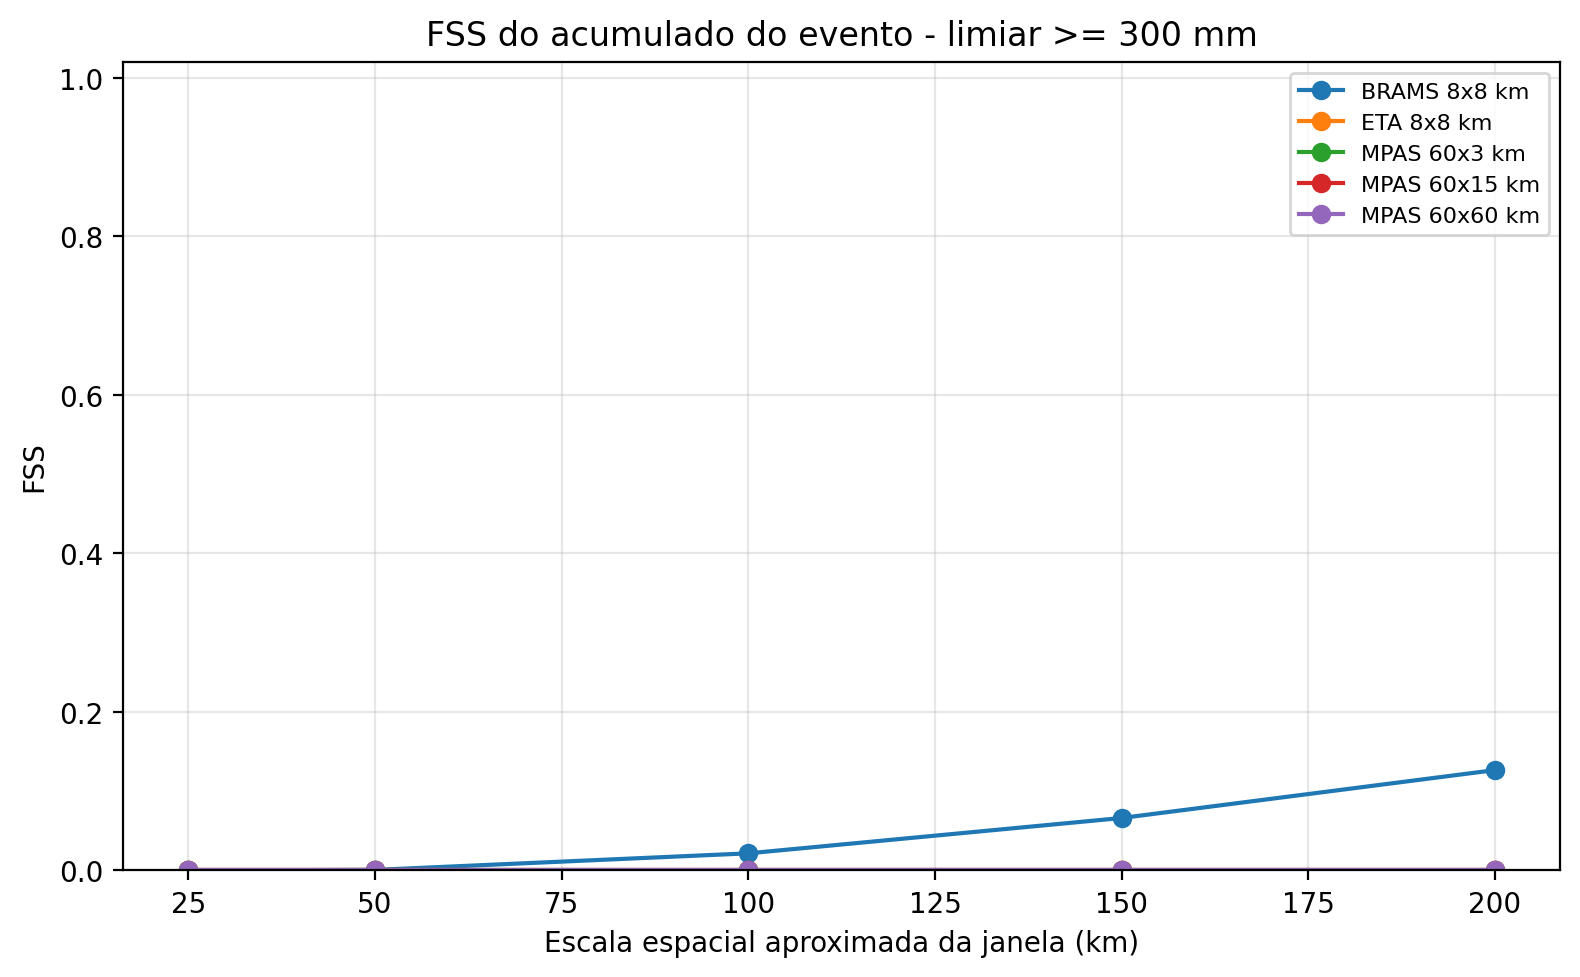
\includegraphics[width=\linewidth,height=0.78\textheight,keepaspectratio]{figuras/5ac725cbe99c52fb6c49d5532768debe8832d59d.png}
\caption{\textcolor{red}{Inserir legenda da figura.}}
\label{fig:figura-45}
\end{figure}

De forma geral, os resultados do FSS reforçam a interpretação obtida na análise qualitativa das previsões brutas. Os modelos apresentaram alguma habilidade para representar a precipitação acumulada mais ampla, principalmente no limiar de 100 mm, mas perderam desempenho de forma acentuada conforme o limiar foi elevado.

Sendo assim, a principal limitação das simulações não esteve apenas na subestimativa dos máximos, mas também no posicionamento inadequado das faixas de maior precipitação. O MPAS 60$\times$60 km apresentou melhor desempenho relativo para a área mais abrangente de chuva acumulada, enquanto o MPAS 60$\times$3 km foi superior nos limiares intermediários de 150 e 200 mm. No entanto, nenhum modelo representou adequadamente os acumulados extremos superiores a 300 mm, indicando baixa habilidade espacial justamente na faixa de precipitação mais relevante para a caracterização do evento.

\section{Análise dos acumulados por bacia.}

Como já citado durante a descrição do evento, no tópico 1.3, a região de estudo não foi igualmente afetada espacialmente, tendo sido mais afetada a região a Região Hidrográfica do Guaíba, como fica evidente pelo mapa de municípios que decretaram estado de calamidade pública durante o evento, apresentado na figura X.

\begin{figure}[H]
\centering
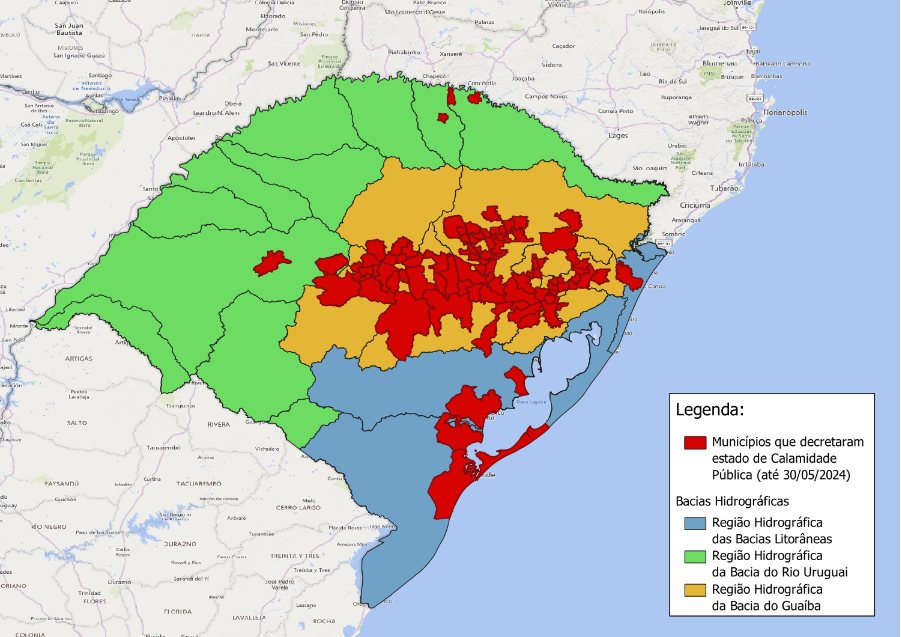
\includegraphics[width=\linewidth,height=0.78\textheight,keepaspectratio]{figuras/3a1ce9beabbbbafc420f9b346c292655dcf1e7c1.png}
\caption{\textcolor{red}{Inserir legenda da figura.}}
\label{fig:figura-46}
\end{figure}

Desta forma, é válida uma análise mais focada nas regiões mais afetadas.

Para isso será analisada a diferença entre a precipitação acumulada média por bacia do produto de precipitação de referência (o MERGE) em comparação com cada um dos modelos, como mostrado na figura Y.

\begin{figure}[H]
\centering
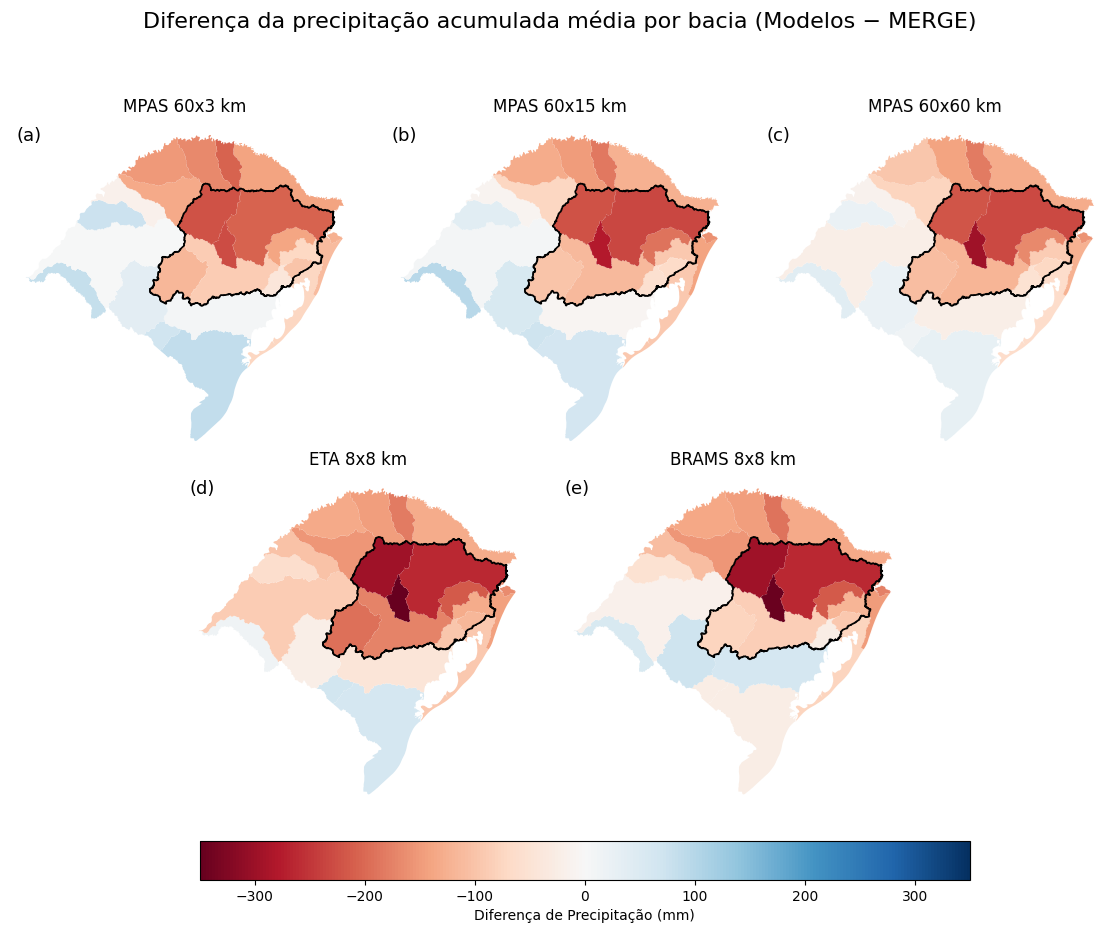
\includegraphics[width=\linewidth,height=0.78\textheight,keepaspectratio]{figuras/fc75db8736987bb98b0d085b37a661cb122765cf.png}
\caption{\textcolor{red}{Inserir legenda da figura.}}
\label{fig:figura-47}
\end{figure}

A análise da diferença da precipitação acumulada média por bacia indica que todos os modelos subestimaram consideravelmente o acumulado total do evento entre 28/04 e 02/05 nas bacias mais afetadas. Entre eles, o MPAS 60$\times$3 km apresentou as menores diferenças negativas, seguido pelo MPAS 60$\times$15 km, MPAS 60$\times$60 km, BRAMS 8 km e ETA 8 km. Assim, embora nenhum modelo tenha reproduzido adequadamente os acumulados observados nessas regiões, as configurações do MPAS apresentaram menor erro médio nas bacias de maior impacto.

Esse resultado também evidencia uma limitação importante de análises fortemente dependentes da localização espacial, como comparações bacia a bacia ou métricas ponto a ponto. Como discutido na seção 5.1.3, modelos que representam parcialmente a estrutura geral da precipitação e seus acumulados, mas apresentam deslocamento espacial relevante, tendem a ser mais penalizados por esse tipo de avaliação. Esse é o caso do BRAMS 8 km, que nas análises qualitativas apresentou desempenho relativamente melhor, ficando em geral atrás apenas do MPAS 60$\times$3 km, mas que, nesta análise por bacia, teve seu desempenho reduzido devido ao deslocamento da faixa principal de precipitação. Enquanto modelos que apresentaram resultados, no geral, piores, como o MPAS 60x60 que suavizou excessivamente os máximos, acabaram sendo beneficiados por manterem valores mais suaves em todo o domínio.

Sendo assim, a diferença entre os resultados qualitativos e a análise por bacia sugere que o desempenho dos modelos deve ser interpretado considerando conjuntamente intensidade, localização e estrutura espacial e que, embora a análise por bacia seja útil para quantificar o erro nas regiões mais impactadas, não deve ser interpretada isoladamente.

\chapter{Conclusão}

Este trabalho avaliou a capacidade do modelo MPAS (em comparação com os modelos ETA e BRAMS) em representar a precipitação associada ao evento extremo ocorrido no Rio Grande do Sul entre o final de abril e o início de maio de 2024. Para isso, foram analisadas duas condições iniciais, em 28 e 29 de abril, com o objetivo de verificar não apenas o desempenho relativo dos modelos, mas também a influência da proximidade temporal da inicialização em relação ao período de maiores acumulados. Antes da comparação com as previsões, o produto MERGE foi avaliado em relação às estações meteorológicas disponíveis e apresentou boa aderência espacial e temporal ao evento, sendo considerado adequado como referência observacional para as análises realizadas.

De forma geral, os resultados indicam que nenhum dos modelos foi capaz de representar adequadamente, ao mesmo tempo, a localização, intensidade e distribuição espacial dos maiores acumulados observados. O MERGE indicou precipitação extrema concentrada principalmente entre o centro-norte, norte e nordeste do Rio Grande do Sul, com áreas superiores a 300 mm no acumulado do evento. Em comparação, as simulações tenderam a deslocar a precipitação para sul ou sudoeste, resultando em subestimativa justamente nas regiões mais afetadas e, em alguns casos, superestimativa relativa em áreas onde os acumulados observados foram menores.

Entre as simulações com condição inicial em 28 de abril, o MPAS 60$\times$3 km apresentou o melhor desempenho qualitativo geral. A configuração de maior resolução representou melhor a estrutura espacial e a intensidade relativa das faixas mais intensas de precipitação, principalmente nos dias finais do evento. Apesar disso, o modelo ainda apresentou erro espacial importante, com deslocamento sistemático da banda principal para sudoeste, além de subestimar a extensão da área com acumulados extremos no total do evento. As configurações MPAS 60$\times$15 km e MPAS 60$\times$60 km representaram bem o padrão geral de distribuição da precipitação, mas apresentaram maior suavização e menor capacidade de reproduzir os núcleos de maior intensidade.

A comparação entre as condições iniciais mostrou que a inicialização mais próxima ao pico do evento não resultou em melhora generalizada das previsões. Pelo contrário, a simulação com condição inicial em 29 de abril apresentou piora no desempenho geral de quase todos os modelos, especialmente no MPAS 60$\times$3 km e no MPAS 60$\times$15 km, que reduziram seus acumulados máximos e subestimaram de forma mais intensa a precipitação nas áreas mais impactadas. O BRAMS foi o único modelo que apresentou melhora nessa condição inicial, com maior área de precipitação intensa e melhor distribuição dos acumulados menores, embora tenha mantido seu principal erro, o deslocamento da faixa principal para sudoeste e concentração exacerbada da faixa precipitante. Sendo assim e, considerando a evolução diária, o acumulado total do evento e a performance geral dos modelos analisados, a simulação com condição inicial em 28 de abril apresentou desempenho mais consistente e foi adotada como simulação padrão para as análises subsequentes.

As análises quantitativas reforçaram a necessidade de interpretar os resultados a partir de múltiplas métricas. A avaliação por bacia indicou subestimativa generalizada dos acumulados nas regiões mais afetadas, com menor diferença média negativa no MPAS 60$\times$3 km. No entanto, também evidenciou que métricas fortemente dependentes da localização espacial penalizam de forma mais intensa modelos que, embora representem acumulados elevados, posicionam incorretamente a faixa principal de precipitação. Esse comportamento foi particularmente evidente no BRAMS, que apresentou desempenho melhor nas outras análises em comparação com os outros modelos, mas foi fortemente penalizado na comparação por bacias devido ao deslocamento espacial dos máximos.

Já o fraction skill score, mostrou que a interpretação do desempenho dos modelos depende fortemente do limiar de precipitação e da escala espacial considerada. Para limiares mais baixos, modelos com campos mais suavizados, como o MPAS 60$\times$60 km, podem apresentar maior habilidade espacial por representarem melhor a abrangência geral da chuva acumulada, embora representem de maneira menos fiel a distribuição espacial dos valores mais intensos. Para limiares mais altos, associados aos núcleos médios e mais intensos do evento, o MPAS 60$\times$3 km apresentou desempenho superior, ainda que necessitando de maior tolerância espacial para atingir valores considerados hábeis. Esse resultado reforça que a maior resolução horizontal e a melhor representação dos processos convectivos contribuíram para uma melhor representação relativa da precipitação intensa, mas não foram suficientes para eliminar erros relevantes de posicionamento e magnitude.

Dessa forma, os resultados indicam que o MPAS 60$\times$3 km apresentou o melhor desempenho geral para a simulação analisada, especialmente na representação da distribuição espacial da precipitação. No entanto, mesmo essa configuração apresentou limitações importantes para a previsão operacional de um evento extremo dessa magnitude, principalmente pela dificuldade em posicionar corretamente os máximos acumulados nas regiões mais afetadas e representar corretamente os valores mais extremos. O ETA 8 km apresentou o pior desempenho geral, com forte subestimativa dos acumulados e baixa aderência espacial ao observado, enquanto o BRAMS 8 km demonstrou capacidade de gerar acumulados elevados, mas com erros relevantes de concentração e deslocamento espacial.

Apesar dessas limitações, as configurações do MPAS, principalmente a de 60$\times$3 km, apresentaram, em todas as métricas analisadas, desempenho comparável ou superior ao dos modelos já amplamente utilizados para previsão de curto prazo no Brasil (o BRAMS e o ETA). Esse resultado é relevante especialmente porque as simulações do MPAS foram realizadas com parametrizações padrão, sem calibração específica, alterações físicas ou adaptações direcionadas ao território brasileiro. Sendo assim, os resultados sugerem que o MPAS apresenta potencial importante para aplicações futuras em previsão de curto prazo e em estudos de eventos extremos no Brasil, ainda que sua utilização operacional dependa de avaliações adicionais para verificar se o bom desempenho relativo se mantém em diferentes cenários.

Além disso, considerando que o MPAS também pode ser aplicado em previsões sazonais, estudos futuros devem avaliar seu desempenho nessa escala temporal em comparação com os modelos frequentemente utilizados para esse tipo de previsão no Brasil. Essa ampliação permitiria verificar se o desempenho relativo observado neste estudo, focado em previsões de curto prazo, também se mantém em horizontes temporais mais longos, especialmente em aplicações voltadas ao monitoramento climático, planejamento setorial e gestão de risco.

\chapter*{Referências}
\markboth{REFERÊNCIAS}{REFERÊNCIAS}
\addcontentsline{toc}{chapter}{Referências}

\begin{enumerate}
\def\labelenumi{\arabic{enumi}.}
\item
  IPCC, 2021: Annex VII: Glossary {[}Matthews, J.B.R., V. Möller, R. van Diemen, J.S. Fuglestvedt, V. Masson-Delmotte, C. Méndez, S. Semenov, A. Reisinger (eds.){]}. In Climate Change 2021: The Physical Science Basis. Contribution of Working Group I to the Sixth Assessment Report of the Intergovernmental Panel on Climate Change {[}Masson-Delmotte, V., P. Zhai, A. Pirani, S.L. Connors, C. Péan, S. Berger, N. Caud, Y. Chen, L. Goldfarb, M.I. Gomis, M. Huang, K. Leitzell, E. Lonnoy, J.B.R. Matthews, T.K. Maycock, T. Waterfield, O. Yelekçi, R. Yu, and B. Zhou (eds.){]}. Cambridge University Press, Cambridge, United Kingdom and New York, NY, USA, pp. 2215--2256, doi:10.1017/9781009157896.022.
\item
  Zhai, Panmao, ed. Guidelines on Climate Watches. Contributions by Walter E. Baethgen, Macol Stewart Cerda, Michael Davey, Premchand Goolaup, Hama Kontongomde, Vernon E. Kousky, Paul Llansó, Chester F. Ropelewski, Phillip Reid, and Panmao Zhai. ©2005, World Meteorological Organization.
\item
  Burroughs, W. J. (n.d.). The natural causes of climate change. Climate Change, 151--199. doi:10.1017/cbo9780511803819.007
\item
  1. Burroughs WJ. The natural causes of climate change. In: Climate Change: A Multidisciplinary Approach. Cambridge University Press; 2007:151-199.
\item
  Diffenbaugh, N. S., \& Burke, M. (2019). \emph{Global warming has increased global economic inequality. Proceedings of the National Academy of Sciences, 201816020.} doi:10.1073/pnas.1816020116
\item
  World Meteorological Organization (WMO). WMO atlas of mortality and economic losses from weather, climate and water extremes (1970--2019). Geneva, 2021. ISBN 978-92-63-11267-5. Available at: \url{https://library.wmo.int/records/item/57564-wmo-atlas-of-mortality-and-economic-losses-from-weather-climate-and-water-extremes-1970-2019}.
\item
  Trenberth, K., Dai, A., van der Schrier, G. et al. Global warming and changes in drought. Nature Clim Change 4, 17--22 (2014). \url{https://doi.org/10.1038/nclimate2067}
\item
  IPCC, 2022: Climate Change 2022: Impacts, Adaptation and Vulnerability. Contribution of Working Group II to the Sixth Assessment Report of the Intergovernmental Panel on Climate Change {[}H.-O. Pörtner, D.C. Roberts, M. Tignor, E.S. Poloczanska, K. Mintenbeck, A. Alegría, M. Craig, S. Langsdorf, S. Löschke, V. Möller, A. Okem, B. Rama (eds.){]}. Cambridge University Press. Cambridge University Press, Cambridge, UK and New York, NY, USA, 3056 pp., doi:10.1017/9781009325844
\item
  IPCC. (2021) Summary for policymakers. In: V. MassonDelmotte, P. Zhai, A. Pirani, S.L. Connors, C. Péan, S. Berger, N. Caud, Y. Chen, L. Goldfarb, M.I. Gomis, M. Huang, K. Leitzell, E. Lonnoy, J.B.R. Matthews, T.K. Maycock, T. Waterfield, O. Yelekçi, R. Yu and B. Zhou (Eds.) Climate Change 2021: The Physical Science Basis. Contribution of Working Group I to the Sixth Assessment Report of the Intergovernmental Panel on Climate Change. Cambridge and New York, NY: Cambridge University Press. (in press).
\item
  Costa, A.A., Guimarães, S.O., Sales, D.C., das Chagas Vasconcelos, F., Junior, Marinho, M.W.S., Pereira, J.M.R. et al. (2022) Precipitation extremes over the tropical Americas under RCP4.5 and RCP8.5 climate change scenarios: results from dynamical downscaling simulations. International Journal of Climatology, 43, 787--803. Available from: \url{https://doi.org/10.1002/joc.7828}
\item
  Marengo, J. A., Jones, R., Alves, L. M., \& Valverde, M. C. (2009). Future change of temperature and precipitation extremes in South America as derived from the PRECIS regional climate modeling system. International Journal of Climatology, 29(15), 2241--2255. doi:10.1002/joc.1863
\item
  Medeiros, F. J. de, Oliveira, C. P. de, \& Avila-Diaz, A. (2022). Evaluation of extreme precipitation climate indices and their projected changes for Brazil: From CMIP3 to CMIP6. \emph{Weather and Climate Extremes}, 38, 100511. ISSN 2212-0947. \url{https://doi.org/10.1016/j.wace.2022.100511}.
\item
  Mantovani, J., Alcântara, E., Pampuch, L.A. et al. Assessing flood risks in the Taquari-Antas Basin (Southeast Brazil) during the September 2023 extreme rainfall surge. npj Nat. Hazards 1, 9 (2024). \url{https://doi.org/10.1038/s44304-024-00009-8}
\item
  PORFÍRIO DA ROCHA, ROSMERI ; \textbf{SIMÕES REBOITA, MICHELLE} ; MACHADO CRESPO, NATÁLIA . Análise do evento extremo de precipitação ocorrido no Rio Grande do Sul entre abril e maio de 2024. JOURNAL HEALTH NPEPS, v. 9, p. e12603, 2024.
\item
  Fonseca, Eliana Lima da; Weber, Eliseu José; Hasenack, Heinrich; Silva, Wallace; Mesquita, Vinícius; Martin, Eduardo Vélez; Schirmbeck, Juliano; Siqueira, João; Ferreira, Bruno; Teixeira Jr., Paulo; Azevedo, Tasso; Shimbo, Julia, 2024, "Nota Técnica sobre os impactos do evento climático de maio de 2024 sobre a cobertura e o uso da terra no Rio Grande do Sul", \url{https://doi.org/10.58053/MapBiomas/1XIXYM}, MapBiomas Data, V1
\item
  DEFESA CIVIL DO RIO GRANDE DO SUL. Defesa Civil atualiza balanço das enchentes no RS -- 08/7. Disponível em: \url{https://www.defesacivil.rs.gov.br/defesa-civil-atualiza-balanco-das-enchentes-no-rs-08-7}. Acesso em: 6 fev. 2025.
\item
  CONFEDERAÇÃO NACIONAL DO COMÉRCIO DE BENS, SERVIÇOS E TURISMO (CNC). Análise dos impactos econômicos da catástrofe no Rio Grande do Sul e do Plano de Reconstrução. 25 jul. 2024. Disponível em: \url{https://www.cncfakeurl.com.br}. Acesso em: 6 fev. 2025.
\item
  ROZANTE, J. R. et al. Combining TRMM and Surface Observations of Precipitation: Technique and Validation over South America. \textbf{Weather and Forecasting}, v. 25, n. 3, p. 885--894, jun. 2010.
\item
  ROZANTE, J. R. et al. Performance of precipitation products obtained from combinations of satellite and surface observations. \textbf{International Journal of Remote Sensing}, v. 41, n. 19, p. 7585--7604, 2020.
\item
  ROZANTE, J. R.; ROZANTE, G. IMERG V07B and V06B: A Comparative Study of Precipitation Estimates Across South America with a Detailed Evaluation of Brazilian Rainfall Patterns. \textbf{Remote Sensing}, v. 16, n. 24, p. 4722, dez. 2024.
\item
  REIS, A. A. et al. Assessing two precipitation data sources at basins of \ldots{} Revista Brasileira de Recursos Hídricos, Porto Alegre, v. 25, e14, 2020. Disponível em: \url{https://www.scielo.br/j/rbrh/a/Q6crdW67brTqgVxG3GQqZWL/}. Acesso em: 09-10-2025. \href{https://www.scielo.br/j/rbrh/a/Q6crdW67brTqgVxG3GQqZWL/?format=pdf&lang=en&utm_source=chatgpt.com}{scielo.br}
\item
  MA, Zhanshan et al. Spin-up characteristics with three types of initial fields and the restart effects on forecast accuracy in the GRAPES global forecast system. Geoscientific Model Development, {[}s.l., v. 14, n. 1, p. 205--221, 12 jan. 2021. DOI: 10.5194/gmd-14-205-2021.
\item
  Chou, S., Dereczynski, C., Gomes, J., Pesquero, J., Ávila, A., Resende, N., De Carvalho, L., Ruiz-Cárdenas, R., De Souza, C., \& Bustamante, J. (2020). Ten-year seasonal climate reforecasts over South America using the Eta Regional Climate Model.. \emph{Anais da Academia Brasileira de Ciências}, 92 3, e20181242 . \url{https://doi.org/10.1590/0001-3765202020181242}.
\item
  Machado, C., Gomes, J., Bustamante, J., Guilhon, L., Cataldi, M., \& Chou, S. (2007). Análise das Previsões de Precipitação Obtidas com a Utilização do Modelo Eta como Insumo para Modelos de Previsão Semanal de Vazão Natural. Revista Brasileira de Recursos Hídricos, 12, 5-12. \url{https://doi.org/10.21168/rbrh.v12n3.p5-12}.
\item
  Freitas, S., Panetta, J., Longo, K., Rodrigues, L., Moreira, D., Rosário, N., Dias, P., Dias, M., Souza, Ê., Freitas, E., Longo, M., Frassoni, A., Fazenda, Á., Silva, C., Pavani, C., Eiras, D., França, D., Massaru, D., Silva, F., Cavalcante, F., Pereira, G., Camponogara, G., Ferrada, G., Velho, H., Menezes, I., Freire, J., Alonso, M., Gácita, M., Zarzur, M., Fonseca, R., Lima, R., Siqueira, R., Braz, R., Tomita, S., Oliveira, V., \& Martins, L. (2016). The Brazilian developments on the Regional Atmospheric Modeling System (BRAMS 5.2): an integrated environmental model tuned for tropical areas.. Geoscientific model development, 10 1, 189-222 . \url{https://doi.org/10.5194/gmd-10-189-2017}.
\item
  Moraes, B., Ferreira, D., Filho, L., Oliveira, J., Souza, E., Júnior, P., Câmara, R., Rocha, E., \& Ribeiro, J. (2013). Comparative Skill of Numerical Weather Forecasts in Eastern Amazonia. Applied Categorical Structures, 03, 355-363. \url{https://doi.org/10.4236/acs.2013.33037}.
\item
  CENTRO DE PREVISÃO DE TEMPO E ESTUDOS CLIMÁTICOS -- CPTEC/INPE. \emph{Data Server: sistema de transferência de dados climáticos e meteorológicos}. Disponível em: \url{https://dataserver.cptec.inpe.br/}. Acesso em: 14 out. 2025.
\item
  GLAHN, Harry R.; LAWRENCE, Bryon. \emph{GRIB2, The WMO standard for the transmission of gridded data: current status and NWS plans}. Silver Spring: National Weather Service/NOAA, 2002. Disponível em: \url{https://www.weather.gov/media/mdl/GlahnLawrence2002GRIB2TheWMOStandard.pdf}. Acesso em: 14 dez. 2025. Serviço Nacional de Meteorologia
\item
  NATIONAL OCEANIC AND ATMOSPHERIC ADMINISTRATION -- NOAA. \emph{Global Forecast System (GFS): numerical forecast system}. Environmental Modeling Center (EMC), National Centers for Environmental Prediction (NCEP). Disponível em: \url{https://www.emc.ncep.noaa.gov/emc/pages/numerical_forecast_systems/gfs.php}. Acesso em: 14 abril 2025. Centro de Modelagem Ambiental
\item
  NATIONAL OCEANIC AND ATMOSPHERIC ADMINISTRATION -- NOAA. \emph{NOMADS: repositório de dados operacionais do Global Forecast System (GFS)}. National Centers for Environmental Prediction (NCEP). Disponível em: \url{https://nomads.ncep.noaa.gov/pub/data/nccf/com/gfs/prod/}. Acesso em: 14 abril 2025.
\item
  NATIONAL CENTER FOR ATMOSPHERIC RESEARCH -- NCAR. \emph{Model for Prediction Across Scales (MPAS): overview}. Mesoscale and Microscale Meteorology Laboratory (MMM). Disponível em: \url{https://www2.mmm.ucar.edu/projects/mpas/site/mpas_overview.html}. Acesso em: 14 Fev. 2025.
\item
  NATIONAL CENTER FOR ATMOSPHERIC RESEARCH -- NCAR. \emph{WRF Preprocessing System (WPS): user's guide}. Mesoscale and Microscale Meteorology Laboratory (MMM). Disponível em: \url{https://www2.mmm.ucar.edu/wrf/users/wrf_users_guide/build/html/wps.html}. Acesso em: 14 Fev. 2025.
\item
  NCAR \textbf{MPAS Tutorial --- Practice Session Guide}. \emph{MPAS-Atmosphere Tutorial}, University Corporation for Atmospheric Research (UCAR) / Mesoscale \& Microscale Meteorology Division. Disponível em: \url{https://www2.mmm.ucar.edu/projects/mpas/tutorial/StAndrews2025/}. Acesso em: 09 10 2025. \href{https://www2.mmm.ucar.edu/projects/mpas/tutorial/StAndrews2025/?utm_source=chatgpt.com}{www2.mmm.ucar.edu}
\item
  UCAR -- UNIVERSITY CORPORATION FOR ATMOSPHERIC RESEARCH. \emph{MPAS-Atmosphere User's Guide}, version 8.2.0. Boulder, CO: National Center for Atmospheric Research, 2023. Disponível em: \url{https://www2.mmm.ucar.edu/projects/mpas/mpas_atmosphere_users_guide_8.2.0.pdf}. Acesso em: 21 11 2025.
\item
  MARENGO, J. A.; DOLIF, G.; CUARTAS, A.; et al. O maior desastre climático do Brasil: chuvas e inundações no estado do Rio Grande do Sul em abril-maio 2024. Estudos Avançados, São Paulo, v. 38, n. 111, 2024. Disponível em: \url{https://www.scielo.br/j/ea/a/LyHVHKHzm67CwpvcWPKPwTm/}. Acesso em: 09 10 2025{]}.
\item
  RIO GRANDE DO SUL. Decreto n\textordmasculine{} 57.646, de 30 de maio de 2024. Altera o Decreto n\textordmasculine{} 57.600, de 4 de maio de 2024, que reitera o estado de calamidade pública no território do Estado do Rio Grande do Sul afetado pelos eventos climáticos de chuvas intensas e especifica os municípios atingidos. Diário Oficial do Estado do Rio Grande do Sul: DOERS, Porto Alegre, 31 maio 2024. Disponível em: \url{https://www.diariooficial.rs.gov.br/materia?id=1002017}. Acesso em: {[}09 10 2025{]}.
\item
  NATIONAL CENTER FOR ATMOSPHERIC RESEARCH (NCAR); MESOSCALE AND MICROSCALE METEOROLOGY LABORATORY (MMM). \textbf{MPAS Atmosphere User Guide: Physics Suites}. Boulder, CO: University Corporation for Atmospheric Research (UCAR), 2024. Disponível em: \url{https://www2.mmm.ucar.edu/projects/mpas/site/documentation/users_guide/phys_suites.html}. Acesso em: 6 jun. 2025.
\item
  Faggian, N., Roux, B., Steinle, P., \& Ebert, B. (2015). Fast calculation of the fractions skill score. MAUSAM, 66(3), 457--466. \url{https://doi.org/10.54302/mausam.v66i3.555}
\item
  Mittermaier, M., Roberts, N., \& Thompson, S. A. (2011). A long-term assessment of precipitation forecast skill using the Fractions Skill Score. Meteorological Applications.
\item
  Roberts, N. M., \& Lean, H. W. (2008). Scale-Selective Verification of Rainfall Accumulations from High-Resolution Forecasts of Convective Events. Monthly Weather Review, 136(1), 78-97. \url{https://doi.org/10.1175/2007MWR2123.1}
\item
  SKOK, Gregor; ROBERTS, Nigel. \textbf{Analysis of Fractions Skill Score properties for random precipitation fields and ECMWF forecasts}. \emph{Quarterly Journal of the Royal Meteorological Society}, v. 142, n. 700, p. 2599--2610, 2016. DOI: 10.1002/qj.2849
\item
  BAUER, P.; THORPE, A.; BRUNET, G. The quiet revolution of numerical weather prediction. Nature, v. 525, n. 7567, p. 47--55, 2015. DOI: 10.1038/nature14956.
\item
  CALEFFI, F.; VIEGAS, C. V.; LIMA, K. B.; BONATO, S. V. Os impactos de eventos climáticos extremos: uma análise abrangente das enchentes de 2024 no Rio Grande do Sul. Redes, v. 29, n. 1, 2024. DOI: 10.17058/redes.v29i1.19660.
\item
  CLOKE, H. L.; PAPPENBERGER, F. Ensemble flood forecasting: a review. Journal of Hydrology, v. 375, n. 3--4, p. 613--626, 2009. DOI: 10.1016/j.jhydrol.2009.06.005.
\item
  DOUVILLE, H. et al. Water cycle changes. In: MASSON-DELMOTTE, V. et al. (Ed.). Climate Change 2021: The Physical Science Basis. Contribution of Working Group I to the Sixth Assessment Report of the Intergovernmental Panel on Climate Change. Cambridge: Cambridge University Press, 2021. cap. 8. DOI: 10.1017/9781009157896.010.
\item
  NEARING, G. et al. Global prediction of extreme floods in ungauged watersheds. Nature, v. 627, n. 8004, p. 559--563, 2024. DOI: 10.1038/s41586-024-07145-1.
\item
  SENEVIRATNE, S. I. et al. Weather and climate extreme events in a changing climate. In: MASSON-DELMOTTE, V. et al. (Ed.). Climate Change 2021: The Physical Science Basis. Contribution of Working Group I to the Sixth Assessment Report of the Intergovernmental Panel on Climate Change. Cambridge: Cambridge University Press, 2021. cap. 11. DOI: 10.1017/9781009157896.013.
\item
  SILVA, J. M. A. et al. Avaliação da performance do modelo ETA nas enchentes de 2024 no Rio Grande do Sul. Revista Brasileira de Ensino de Ciências e Matemática, v. 7, n. 2, 2024. DOI: 10.15536/reducarmais.7.2024.28280.
\item
  PETRY, I.; MIRANDA, P. T.; PAIVA, R. C. D.; COLLISCHONN, W.; FAN, F. M.; FAGUNDES, H. O.; ARAUJO, A. A.; SOUZA, S. Changes in flood magnitude and frequency projected for vulnerable regions and major wetlands of South America. \textbf{Geophysical Research Letters}, v. 52, n. 5, p. e2024GL112436, mar. 2025. DOI: \href{https://doi.org/10.1029/2024GL112436}{10.1029/2024GL112436}.
\item
  BUSKER, T.; VAN DEN HURK, B.; DE MOEL, H.; AERTS, J. C. J. H. The value of precipitation forecasts to anticipate floods. \textbf{Bulletin of the American Meteorological Society}, v. 106, n. 3, p. E473--E491, mar. 2025. DOI: \href{https://doi.org/10.1175/BAMS-D-24-0073.1}{10.1175/BAMS-D-24-0073.1}.
\item
  Pu Z., Kalnay E. (2018) Numerical Weather Prediction Basics: Models, Numerical Methods, and Data Assimilation. In: Duan Q., Pappenberger F., Thielen J., Wood A., Cloke H., Schaake J. (eds) Handbook of Hydrometeorological Ensemble Forecasting. Springer, Berlin, Heidelberg
\item
  KÜHNLEIN, Christian; SMOLARKIEWICZ, Piotr K. A nonhydrostatic finite-volume option for the IFS. ECMWF Newsletter, n. 158, p. 30--36, winter 2018/19. DOI: 10.21957/sd92ack6p3. Disponível em: \url{https://www.ecmwf.int/sites/default/files/elibrary/2019/18884-nonhydrostatic-finite-volume-option-ifs.pdf}. Acesso em: 22 jun. 2025.
\item
  WEDI, N. P.; BAUER, P.; DECONINCK, W.; DIAMANTAKIS, M.; HAMRUD, M.; KÜHNLEIN, C.; MALARDEL, S.; MOGENSEN, K.; MOZDZYNSKI, G.; SMOLARKIEWICZ, P. K. The modelling infrastructure of the Integrated Forecasting System: recent advances and future challenges. Reading: European Centre for Medium-Range Weather Forecasts, 2015. ECMWF Technical Memorandum, n. 760. Disponível em: \url{https://www.ecmwf.int/sites/default/files/elibrary/2015/15259-modelling-infrastructure-integrated-forecasting-system-recent-advances-and-future-challenges.pdf}. Acesso em: 22 jun. 2025.
\item
  DAVIES, Terry. \textbf{Lateral boundary conditions for limited area models}. \emph{Quarterly Journal of the Royal Meteorological Society}, v. 140, n. 678, p. 185--196, 2014. DOI: 10.1002/qj.2127.
\item
  TAPIADOR, Francisco J.; NAVARRO, Andrés; MORENO, Raúl; SÁNCHEZ, José Luis; GARCÍA-ORTEGA, Eduardo. \textbf{Regional climate models: 30 years of dynamical downscaling}. \emph{Atmospheric Research}, v. 235, artigo 104785, 2020. DOI: 10.1016/j.atmosres.2019.104785.
\item
  Feser, F.; Rockel, B.; von Storch, H.; Winterfeldt, J.; Zahn, M. Regional Climate Models Add Value to Global Model Data: A Review and Selected Examples. Bulletin of the American Meteorological Society, 92(9), 1181-1192, 2011. DOI: 10.1175/2011BAMS3061.1. URL: \url{https://www.hereon.de/imperia/md/content/gkss/zentrale_einrichtungen/bibliothek/journals/2011/feser_29114.pdf}
\item
  GIORGI, Filippo; GUTOWSKI JR., William J. \textbf{Regional dynamical downscaling and the CORDEX initiative}. \emph{Annual Review of Environment and Resources}, v. 40, p. 1.1--1.24, 2015. DOI: 10.1146/annurev-environ-102014-021217.
\item
  Chou, S. C.; Justi da Silva, M. G. A. \emph{Objective evaluation of Eta Model precipitation forecasts over South America}. Revista Climanálise, ano 1, n. 1, 1999. URL: \url{http://climanalise.cptec.inpe.br/~rclimanl/revista/pdf/ETA_Chou.pdf}
\item
  Freitas, S. R. et al. \emph{The Brazilian developments on the Regional Atmospheric Modeling System (BRAMS 5.2): an integrated environmental model tuned for tropical areas}. Geoscientific Model Development, 10, 189-222, 2017. DOI: 10.5194/gmd-10-189-2017. URL: \url{https://gmd.copernicus.org/articles/10/189/2017/}
\item
  SKAMAROCK, William C.; KLEMP, Joseph B.; DUDA, Michael G.; FOWLER, Laura D.; PARK, Sang-Hun; RINGLER, Todd D. \textbf{A multiscale nonhydrostatic atmospheric model using centroidal Voronoi tesselations and C-grid staggering}. \emph{Monthly Weather Review}, v. 140, n. 9, p. 3090--3105, 2012. DOI: 10.1175/MWR-D-11-00215.1.
\item
  PARK, Sang-Hun; KLEMP, Joseph B.; SKAMAROCK, William C. \textbf{A comparison of mesh refinement in the global MPAS-A and WRF models using an idealized normal-mode baroclinic wave simulation}. \emph{Monthly Weather Review}, v. 142, n. 10, p. 3614--3634, 2014. DOI: 10.1175/MWR-D-14-00004.1.
\item
  NATIONAL CENTERS FOR ENVIRONMENTAL PREDICTION. Environmental Modeling Center. Global Forecast System (GFS). College Park: NCEP/EMC, {[}s.d.. Disponível em: \url{https://www.emc.ncep.noaa.gov/emc/pages/numerical_forecast_systems/gfs.php}. Acesso em: 22 abr. 2026.
\item
  NATIONAL CENTERS FOR ENVIRONMENTAL PREDICTION. NWS Central Operations. NCEP products inventory: global products. College Park: NCEP/NCO, 2024. Disponível em: \url{https://www.nco.ncep.noaa.gov/pmb/products/gfs/}. Acesso em: 22 abr. 2026.
\item
  BLACK, T. L. The new NMC mesoscale Eta model: Description and forecast examples. Weather and Forecasting, v. 9, n. 2, p. 265-278, 1994. DOI:10.1175/1520-0434(1994)009\textless0265:TNNMEM\textgreater2.0.CO;2.
\item
  CHOU, S. C.; BUSTAMANTE, J. F.; GOMES, J. L. Evaluation of Eta Model seasonal precipitation forecasts over South America. Nonlinear Processes in Geophysics, v. 12, p. 537-555, 2005. DOI: 10.5194/npg-12 537-2005.
\item
  CHOU, S. C. et al. Downscaling of South America present climate driven by 4-member HadCM3 runs. Climate Dynamics, v. 38, p. 635-653, 2012. DOI: 10.1007/s00382-011-1002-8.
\item
  CHOU, S. C. et al. Ten-year seasonal climate reforecasts over South America using the Eta Regional Climate Model. Anais da Academia Brasileira de Ciências, v. 92, n. 3, e20181242, 2020. DOI: 10.1590/0001-3765202020181242.
\item
  DERECZYNSKI, C. et al. Downscaling of climate extremes over South America - Part I: model evaluation in the reference climate. Weather and Climate Extremes, v. 29, 100273, 2020. DOI: 10.1016/j.wace.2020.100273.
\item
  EK, M. B. et al. Implementation of Noah land surface model advances in the National Centers for Environmental Prediction operational mesoscale Eta model. Journal of Geophysical Research: Atmospheres, v. 108, n. D22, 8851, 2003. DOI: 10.1029/2002JD003296.
\item
  JANJIĆ, Z. I. The Step-Mountain Eta Coordinate Model: further developments of the convection, viscous sublayer, and turbulence closure schemes. Monthly Weather Review, v. 122, n. 5, p. 927-945, 1994. DOI: 10.1175/1520-0493(1994)122\textless0927:TSMECM\textgreater2.0.CO;2.
\item
  KAIN, J. S. The Kain-Fritsch convective parameterization: an update. Journal of Applied Meteorology, v. 43, n. 1, p. 170-181, 2004. DOI: 10.1175/1520-0450(2004)043\textless0170:TKCPAU\textgreater2.0.CO;2.
\item
  LYRA, A. A. et al. Manual Modelo Eta - Versão 1.4.2. Brasil: INPE/CPTEC, setembro de 2022.
\item
  MARENGO, J. A. et al. Development of regional future climate change scenarios in South America using the Eta CPTEC/HadCM3 climate change projections: climatology and regional analyses for the Amazon, São Francisco and the Paraná River basins. Climate Dynamics, v. 38, p. 1829-1848, 2012. DOI: 10.1007/s00382-011-1155-5.
\item
  MESINGER, F. A blocking technique for representation of mountains in atmospheric models. Rivista di Meteorologia Aeronautica, v. 44, p. 195-202, 1984.
\item
  MESINGER, F. et al. The step-mountain coordinate: model description and performance for cases of Alpine lee cyclogenesis and for a case of Appalachian redevelopment. Monthly Weather Review, v. 116, n. 7, p. 1493-1518, 1988. DOI: 10.1175/1520-0493(1988)116\textless1493:TSMCMD\textgreater2.0.CO;2.
\item
  MESINGER, F. et al. An upgraded version of the Eta model. Meteorology and Atmospheric Physics, v. 116, p. 63-79, 2012. DOI: 10.1007/s00703-012-0182-z.
\item
  MOURA, R. G.; HERDIES, D. L.; MENDES, D.; MENDES, M. C. D. Avaliação do modelo regional Eta utilizando as análises do CPTEC e NCEP. Revista Brasileira de Meteorologia, v. 25, n. 1, p. 46-53, 2010. DOI: 10.1590/S0102-77862010000100005.
\item
  PESQUERO, J. F.; CHOU, S. C.; NOBRE, C. A.; MARENGO, J. A. Climate downscaling over South America for 1961-1970 using the Eta Model. Theoretical and Applied Climatology, v. 99, p. 75-93, 2010. DOI: 10.1007/s00704-009-0123-z.
\item
  TAVARES, P. S. et al. Dynamical-statistical downscaling of seasonal hindcasts of temperature and precipitation over South America. Revista Brasileira de Recursos Hídricos, v. 30, e7, 2025. DOI: 10.1590/2318-0331.302520240073.
\item
  VIEIRA, R. M. G. et al. Avaliação das previsões de precipitação do Modelo Eta para Bacia do Rio São Francisco em Minas Gerais, Brasil. Anuário do Instituto de Geociências - UFRJ, v. 38, n. 2, p. 15-23, 2015. DOI: 10.11137/2015\_2\_15\_23.
\item
  COTTON, W. R.; PIELKE SR., R. A.; WALKO, R. L.; LISTON, G. E.; TREMBACK, C. J.; JIANG, H.; MCANELLY, R. L.; HARRINGTON, J. Y.; NICHOLLS, M. E.; CARRIO, G. G.; MCFADDEN, J. P. RAMS 2001: current status and future directions. \emph{Meteorology and Atmospheric Physics}, v. 82, p. 5-29, 2003.
\item
  DOS SANTOS, A. F.; FREITAS, S. R.; DE MATTOS, J. G. Z.; DE CAMPOS VELHO, H. F.; GAN, M. A.; DA LUZ, E. F. P.; GRELL, G. A. Using the Firefly optimization method to weight an ensemble of rainfall forecasts from the Brazilian developments on the Regional Atmospheric Modeling System (BRAMS). \emph{Advances in Geosciences}, v. 35, p. 123-136, 2013. DOI: 10.5194/adgeo-35-123-2013.
\item
  FREITAS, S. R.; LONGO, K. M.; SILVA DIAS, M. A. F.; CHATFIELD, R.; SILVA DIAS, P.; ARTAXO, P.; ANDREAE, M. O.; GRELL, G.; RODRIGUES, L. F.; FAZENDA, A.; PANETTA, J. The Coupled Aerosol and Tracer Transport model to the Brazilian developments on the Regional Atmospheric Modeling System (CATT-BRAMS): Part 1: model description and evaluation. \emph{Atmospheric Chemistry and Physics}, v. 9, p. 2843-2861, 2009. DOI: 10.5194/acp-9-2843-2009.
\item
  FREITAS, S. R.; PANETTA, J.; LONGO, K. M.; RODRIGUES, L. F.; MOREIRA, D. S.; ROSÁRIO, N. E.; SILVA DIAS, P. L.; SILVA DIAS, M. A. F.; SOUZA, E. P.; FREITAS, E. D.; et al. The Brazilian developments on the Regional Atmospheric Modeling System (BRAMS 5.2): an integrated environmental model tuned for tropical areas. \emph{Geoscientific Model Development}, v. 10, p. 189-222, 2017. DOI: 10.5194/gmd-10-189-2017.
\item
  FREITAS, S. R.; RODRIGUES, L. F.; PANETTA, J.; LONGO, K. M.; MOREIRA, D.; FREITAS, E.; LONGO, M.; FAZENDA, A.; FONSECA, R.; STOCKLER, R.; CAMPONOGARA, G. \emph{Brazilian developments on the Regional Atmospheric Modeling System BRAMS version 5.2: description of the model input namelist parameters}. Cachoeira Paulista: CPTEC/INPE, 2016. Manual técnico, edição 1.0.
\item
  FREITAS, S. R.; RODRIGUES, L. F.; LONGO, K. M.; PANETTA, J. Impact of a monotonic advection scheme with low numerical diffusion on transport modeling of emissions from biomass burning. \emph{Journal of Advances in Modeling Earth Systems}, v. 4, M01001, 2012. DOI: 10.1029/2011MS000084.
\item
  GARCÍA VILLANUEVA, J.; SUTIZAL SÁNCHEZ, B. A. Uso del modelo ``Brazilian Regional Atmospheric Modeling System'' (BRAMS) en el análisis del huaico de Chosica en Lima Perú. \emph{Anales Científicos}, v. 78, n. 2, p. 157-172, 2017. DOI: 10.21704/ac.v78i2.1053.
\item
  GRELL, G. A.; DÉVÉNYI, D. A generalized approach to parameterizing convection combining ensemble and data assimilation techniques. \emph{Geophysical Research Letters}, v. 29, n. 14, p. 38-1-38-4, 2002. DOI: 10.1029/2002GL015311.
\item
  GRELL, G. A.; FREITAS, S. R. A scale and aerosol aware stochastic convective parameterization for weather and air quality modeling. \emph{Atmospheric Chemistry and Physics}, v. 14, p. 5233-5250, 2014. DOI: 10.5194/acp-14-5233-2014.
\item
  LONGO, K. M.; FREITAS, S. R.; ANDREAE, M. O.; SETZER, A.; PRINS, E.; ARTAXO, P. The Coupled Aerosol and Tracer Transport model to the Brazilian developments on the Regional Atmospheric Modeling System (CATT-BRAMS): Part 2: model sensitivity to the biomass burning inventories. \emph{Atmospheric Chemistry and Physics}, v. 10, p. 5785-5795, 2010. DOI: 10.5194/acp-10-5785-2010.
\item
  MEDVIGY, D.; MOORCROFT, P. R.; AVISSAR, R.; WALKO, R. L. Mass conservation and atmospheric dynamics in the Regional Atmospheric Modeling System (RAMS). \emph{Environmental Fluid Mechanics}, v. 5, p. 109-134, 2005. DOI: 10.1007/s10652-005-5275-5.
\item
  MORAES, B. C. de; FERREIRA, D. B. da S.; MEIRA FILHO, L. G.; OLIVEIRA, J. V. de; SOUZA, E. B. de; FERREIRA JÚNIOR, P. P.; CÂMARA, R. K. C.; ROCHA, E. J. P. da; RIBEIRO, J. B. M. Comparative Skill of Numerical Weather Forecasts in Eastern Amazonia. \emph{Atmospheric and Climate Sciences}, v. 3, p. 355-363, 2013. DOI: 10.4236/acs.2013.33037.
\item
  MOREIRA, D. S.; FREITAS, S. R.; BONATTI, J. P.; MERCADO, L. M.; ROSÁRIO, N. M. É.; LONGO, K. M.; MILLER, J. B.; GLOOR, M.; GATTI, L. V. Coupling between the JULES land-surface scheme and the CCATT-BRAMS atmospheric chemistry model (JULES-CCATT-BRAMS1.0): applications to numerical weather forecasting and the CO₂ budget in South America. \emph{Geoscientific Model Development}, v. 6, p. 1243-1259, 2013. DOI: 10.5194/gmd-6-1243-2013.
\item
  PIELKE, R. A.; COTTON, W. R.; WALKO, R. L.; TREMBACK, C. J.; LYONS, W. A.; GRASSO, L. D.; NICHOLLS, M. E.; MORAN, M. D.; WESLEY, D. A.; LEE, T. J.; COPELAND, J. H. A comprehensive meteorological modeling system: RAMS. \emph{Meteorology and Atmospheric Physics}, v. 49, p. 69-91, 1992.
\item
  TRIPOLI, G. J.; COTTON, W. R. The Colorado State University three-dimensional cloud/mesoscale model. Part I: General theoretical framework and sensitivity experiments. \emph{Journal de Recherches Atmosphériques}, v. 16, p. 185-220, 1982.
\item
  WALCEK, C. J. Minor flux adjustment near mixing ratio extremes for simplified yet highly accurate monotonic calculation of tracer advection. \emph{Journal of Geophysical Research}, v. 105, p. 9335-9348, 2000. DOI: 10.1029/1999JD901142.
\item
  BECK, H. E. et al. Global-scale evaluation of 22 precipitation datasets using gauge observations and hydrological modeling. Hydrology and Earth System Sciences, v. 21, p. 6201-6217, 2017. DOI: 10.5194/hess-21-6201-2017.
\item
  COSTA, J. C. et al. Validação dos dados de precipitação estimados pelo CHIRPS para o Brasil. Revista Brasileira de Climatologia, v. 24, p. 228-243, 2019. DOI: 10.5380/abclima.v24i0.60237.
\item
  FENG, Z. et al. Evaluation of Mesoscale Convective Systems in Climate Simulations: Methodological Development and Results from MPAS-CAM over the United States. Journal of Climate, v. 34, n. 7, p. 2611-2633, 2021. DOI: 10.1175/JCLI-D-20-0136.1.
\item
  FOWLER, L. D. et al. Analyzing the Grell-Freitas convection scheme from hydrostatic to nonhydrostatic scales within a global model. Monthly Weather Review, v. 144, n. 6, p. 2285-2306, 2016. DOI: 10.1175/MWR-D-15-0311.1.
\item
  FREITAS, S. R. de. Model for Ocean-laNd-Atmosphere Prediction (MONAN): avaliação dos candidatos ao núcleo dinâmico do componente atmosférico (MONAN-ATM) - recomendação ao Comitê Científico do MONAN. São José dos Campos: INPE, 2023. Disponível em: \url{http://urlib.net/8JMKD3MGP3W34T/49MKML8}. Acesso em: 24 jun. 2026.
\item
  FUSINATO, B. Exploring cold pools dynamics in MONAN: insights from numerical simulations of hurricanes. 2025. Dissertação (Mestrado em Meteorologia) - Instituto Nacional de Pesquisas Espaciais, São José dos Campos, 2025. Disponível em: \url{http://urlib.net/8JMKD2USNRW34T/4E6PL2B}. Acesso em: 24 jun. 2026.
\item
  GILLIAM, R. C. et al. Establishing the suitability of the Model for Prediction Across Scales for global retrospective air quality modeling. Journal of Geophysical Research: Atmospheres, v. 126, n. 10, e2020JD033588, 2021. DOI: 10.1029/2020JD033588.
\item
  GRELL, G. A.; FREITAS, S. R. A scale and aerosol aware stochastic convective parameterization for weather and air quality modeling. Atmospheric Chemistry and Physics, v. 14, p. 5233-5250, 2014. DOI: 10.5194/acp-14-5233-2014.
\item
  GUERRETTE, J. J. et al. Data assimilation for the Model for Prediction Across Scales - Atmosphere with the Joint Effort for Data Assimilation Integration (JEDI-MPAS 2.0.0-beta): ensemble of 3D ensemble-variational (En-3DEnVar) assimilations. Geoscientific Model Development, v. 16, p. 7123-7142, 2023. DOI: 10.5194/gmd-16-7123-2023.
\item
  HAGOS, S. et al. Error characteristics of two grid refinement approaches in aquaplanet simulations: MPAS-A and WRF. Monthly Weather Review, v. 141, n. 9, p. 3022-3036, 2013. DOI: 10.1175/MWR-D-12-00338.1.
\item
  HEINZELLER, D.; DUDA, M. G.; KUNSTMANN, H. Towards convection-resolving, global atmospheric simulations with the Model for Prediction Across Scales (MPAS) v3.1: an extreme scaling experiment. Geoscientific Model Development, v. 9, p. 77-110, 2016. DOI: 10.5194/gmd-9-77-2016.
\item
  KHAMIS, E. G. et al. Aspectos computacionais e de operacionalização do MONAN-Model versão 1.4.3-RC. São José dos Campos: INPE, 2026. Disponível em: \url{http://urlib.net/8JMKD2USNRW34T/4FPGQE8}. Acesso em: 24 jun. 2026.
\item
  KUBOTA, P. Y. et al. Relatório técnico: perspectivas da modelagem numérica dos processos de microfísica de nuvens no Brasil e suas aplicações no modelo comunitário MONAN. São José dos Campos: INPE, 2023. Disponível em: \url{http://urlib.net/8JMKD3MGP3W34T/49RSTC5}. Acesso em: 24 jun. 2026.
\item
  KLEMP, J. B.; SKAMAROCK, W. C.; DUDHIA, J. Conservative split-explicit time integration methods for the compressible nonhydrostatic equations. Monthly Weather Review, v. 135, n. 8, p. 2897-2913, 2007. DOI: 10.1175/MWR3440.1.
\item
  LIANG, Y. et al. Multiscale simulation of precipitation over East Asia by variable resolution CAM-MPAS. Journal of Advances in Modeling Earth Systems, v. 13, n. 11, e2021MS002656, 2021. DOI: 10.1029/2021MS002656.
\item
  LIU, Z. et al. Data assimilation for the Model for Prediction Across Scales - Atmosphere with the Joint Effort for Data Assimilation Integration (JEDI-MPAS 1.0.0): EnVar implementation and evaluation. Geoscientific Model Development, v. 15, p. 7859-7878, 2022. DOI: 10.5194/gmd-15-7859-2022.
\item
  LUI, Y. S. et al. Performance of MPAS-A and WRF in predicting and simulating western North Pacific tropical cyclone tracks and intensities. Theoretical and Applied Climatology, v. 143, p. 505-520, 2021. DOI: 10.1007/s00704-020-03444-5.
\item
  MICHAELIS, A. C.; LACKMANN, G. M.; ROBINSON, W. A. Evaluation of a unique approach to high-resolution climate modeling using the Model for Prediction Across Scales - Atmosphere (MPAS-A) version 5.1. Geoscientific Model Development, v. 12, p. 3725-3743, 2019. DOI: 10.5194/gmd-12-3725-2019.
\item
  MONAN. MONAN (Model for Ocean-laNd-Atmosphere PredictioN). 2026. Disponível em: \url{https://monanadmin.github.io/}. Acesso em: 24 abr. 2026.
\item
  MPAS DEVELOPMENT TEAM. MPAS-Model README. GitHub repository. 2026a. Disponível em: \url{https://github.com/MPAS-Dev/MPAS-Model}. Acesso em: 24 abr. 2026.
\item
  MPAS DEVELOPMENT TEAM. MPAS Atmosphere overview. 2026b. Disponível em: \url{https://mpas-dev.github.io/atmosphere/atmosphere.html}. Acesso em: 24 abr. 2026.
\item
  MPAS DEVELOPMENT TEAM. MPAS-Atmosphere Model User\textquotesingle s Guide, Version 8.4.0. Boulder: NSF NCAR, 2026c. Disponível em: \url{https://www2.mmm.ucar.edu/projects/mpas/mpas_atmosphere_users_guide_8.4.0.pdf}. Acesso em: 24 abr. 2026.
\item
  MPAS DEVELOPMENT TEAM. MPAS-Atmosphere public releases and downloads. 2026d. Disponível em: \url{https://mpas-dev.github.io/atmosphere/atmosphere_download.html}. Acesso em: 24 abr. 2026.
\item
  MPAS TUTORIAL TEAM. MPAS-Atmosphere tutorial: Practice Session Guide. NSF NCAR, 2024. Disponível em: \url{https://www2.mmm.ucar.edu/projects/mpas/tutorial/Howard2024/index.html}. Acesso em: 25 abr. 2026.
\item
  PARK, S.-H.; KLEMP, J. B.; SKAMAROCK, W. C. A comparison of mesh refinement in the global MPAS-A and WRF models using an idealized normal-mode baroclinic wave simulation. Monthly Weather Review, v. 142, n. 10, p. 3614-3634, 2014. DOI: 10.1175/MWR-D-14-00004.1.
\item
  RINGLER, T. D. et al. A unified approach to energy conservation and potential vorticity dynamics for arbitrarily-structured C-grids. Journal of Computational Physics, v. 229, n. 9, p. 3065-3090, 2010. DOI: 10.1016/j.jcp.2009.12.007.
\item
  RINGLER, T. D. et al. Exploring a multiresolution modeling approach within the shallow-water equations. Monthly Weather Review, v. 139, n. 11, p. 3348-3368, 2011. DOI: 10.1175/MWR-D-10-05049.1.
\item
  RODRIGUES, L. F. et al. Avaliação computacional de núcleos dinâmicos candidatos para o MONAN. São José dos Campos: INPE, 2023. Disponível em: \url{http://urlib.net/8JMKD3MGP3W34T/49MKMSS}. Acesso em: 24 jun. 2025.
\item
  SÁ, R. V. de. Model for Prediction Across Scales (MPAS) usado na modelagem atmosférica em multiescala e nas previsões de tempo, operacional e curto prazo para o Brasil. 2023. Tese (Doutorado em Ciências) - Programa de Engenharia Mecânica, COPPE, Universidade Federal do Rio de Janeiro, Rio de Janeiro, 2023.
\item
  SKAMAROCK, W. C.; GASSMANN, A. Conservative transport schemes for spherical geodesic grids: high-order flux operators for ODE-based time integration. Monthly Weather Review, v. 139, n. 9, p. 2962-2975, 2011. DOI: 10.1175/MWR-D-10-05056.1.
\item
  SKAMAROCK, W. C. et al. A multiscale nonhydrostatic atmospheric model using centroidal Voronoi tesselations and C-grid staggering. Monthly Weather Review, v. 140, n. 9, p. 3090-3105, 2012. DOI: 10.1175/MWR-D-11-00215.1.
\item
  THUBURN, J. et al. Numerical representation of geostrophic modes on arbitrarily structured C-grids. Journal of Computational Physics, v. 228, n. 22, p. 8321-8335, 2009. DOI: 10.1016/j.jcp.2009.08.006.
\item
  REBOITA, Michelle Simões; MATTOS, Enrique Vieira; CAPUCIN, Bruno Cesar; SOUZA, Diego Oliveira de; FERREIRA, Glauber Willian de Souza. A multi-scale analysis of the extreme precipitation in Southern Brazil in April/May 2024. Atmosphere, v. 15, n. 9, artigo 1123, 2024. DOI: 10.3390/atmos15091123.
\item
  REHBEIN, Amanda; DUTRA, Lais Martins; AMBRIZZI, Tercio; ROCHA, Rosmeri Porfírio da; REBOITA, Michelle Simões; SILVA, Gustavo Alves da; GOZZO, Luiz Felipe; TOMAZIELLO, Ana Carolina; CAMPOS, José Luiz; MAYTA, Victor R.; CRESPO, Natália Machado; BUENO, Patrícia G.; ALIAGA NESTARES, Vanessa J.; MACHADO, Luiz Teixeira; JESUS, Eder Márcio de; PAMPUCH, Lívia A.; CUSTÓDIO, Maria de; CARPENEDO, Camila Bertoletti; LUPO, Anthony R. Severe weather events over Southeastern Brazil during the 2016 dry season. Advances in Meteorology, v. 2018, artigo 4878503, 2018. DOI: 10.1155/2018/4878503.
\item
  YUSSOUF, Nusrat; KNOPFMEIER, Katherine H. Application of the Warn-on-Forecast system for flash-flood-producing heavy convective rainfall events. Quarterly Journal of the Royal Meteorological Society, v. 145, n. 723, p. 2385-2403, 2019. DOI: 10.1002/qj.3568.
\item
  ROSSA, A.; NURMI, P.; EBERT, E. \textbf{Overview of methods for the verification of quantitative precipitation forecasts}. In: MICHAELIDES, S. (ed.). \emph{Precipitation: Advances in Measurement, Estimation and Prediction}. Berlin, Heidelberg: Springer, 2008. p. 419--452. DOI: 10.1007/978-3-540-77655-0\_16.
\item
  MAPBIOMAS. \textbf{Nota técnica: os impactos do evento climático de maio de 2024 sobre a cobertura e o uso da terra no Rio Grande do Sul}. 2024. Disponível em: \url{https://brasil.mapbiomas.org/wp-content/uploads/sites/4/2024/06/NT\_Evento\_climatico\_extremo\_RS\_maio\_2024\_Final.pptx.pdf}. Acesso em: 25 jun. 2025.
\end{enumerate}

\end{document}
